\chapter{Spin \& Parity of a Higgs Boson}
\label{sec:Spin_Experiment}
\chaptermark{Spin \& Parity of a Higgs Boson}

In this thesis, an extensive study of the spin-parity properties of the Higgs boson and of the tensor structure of its interactions with electroweak gauge bosons is presented using the $H \to ZZ/Z\gamma^*/\gamma^*\gamma^*\to4\ell$ decay channel, where the interference between the three intermediate states is included. The study focuses on testing for the presence of anomalous effects in $HZZ$ and interactions under spin-zero, -one, and -two hypotheses, but also probes the $Z\gamma^*$ or $\gamma^*\gamma^*\to4\ell$ terms. Constraints are set on eight anomalous coupling contributions to the $HVV$ interactions\footnote{Eleven when the $HWW$ extensions are included.}, where $V$ is a gauge vector boson, under the spin-zero assumption of the Higgs boson. Extending the exclusion of $0^{-}\left(2_{m}^{+}\right)$ hypotheses in favor of the SM and the original measurement of the $f_{a3}$ parameter \cite{Chatrchyan:2012jja}, this thesis work developed the most comprehensive study of the spin-parity and tensor structure measurements to date. These studies have been published in \cite{Chatrchyan:2013mxa} and submitted for publication in \cite{Khachatryan:2014kca}. A summary of the measurements performed is outlined in the first section, a summary of the simulated data and four lepton event selection is discussed, then an description of the analysis techniques is given. Finally, the results of this analysis are presented. The results section first presents spin-one and spin-two exclusions followed by the study of spin-zero $HVV$ couplings.

\section{Summary of Spin/Parity Measurements}
\label{sec:General_Spin_Parity}

The analysis is based on theoretical and phenomenological studies that describe the couplings of a Higgs-like boson to two gauge bosons presented in section \ref{sec:Higgs_Spin_Pheno}. They provide techniques and ideas for measuring the spin and $CP$ properties of a particle interacting with vector bosons~\cite{Gao:2010qx,Bolognesi:2012mm,Anderson:2013afp}. Much of the relevant phenomenological introduction has already been presented, but here we summarize the tests performed.

For spin-zero tests are performed to measure the effective cross section fractions $f_{i}^{VV}$. The analysis studies the effects of the anomalous couplings listed in table \ref{tab:xsec_ratio} are tested where the mass of the hypothesized boson is assumed to be $m_{H} = \unit{125.6}{\GeV}$ \cite{Chatrchyan:2013mxa}. When testing the $HZZ$ terms, the superscript is dropped from the fraction definition to be consistent with earlier publications. In this table $WW$ terms are listed, they are also tested following the phenomenological work in this thesis and as part of the analysis presented in \cite{Khachatryan:2014kca}, but are beyond the scope of this thesis. Given the measured values of the effective fractions, it is possible to extract the ratios of the coupling constants $a_i/a_1$, the scale of BSM physics $\Lambda_{1}$, or the ratios of the $Z\gamma^*$ ($\gamma^*\gamma^*$) cross sections with respect to the SM predictions in any parameterization.


\begin{table}
\centering
\caption[List of anomalous $HVV$ couplings considered in the measurements assuming a spin-zero Higgs boson. The definition of the effective fractions is discussed in the text and the translation constant is given in each case. The effective cross sections correspond to the processes $H \to VV \to 2e2\mu$ and the Higgs boson mass $m_{H}=\unit{125.6}{\GeV}$ using the \textsc{JHUGen} calculation. The cross-section ratios for the $HZ\gamma$ and $H\gamma\gamma$ couplings include the requirement $\sqrt{q^2_{V}} \ge \unit{4}{\GeV}$.]{
List of anomalous $HVV$ couplings considered in the measurements assuming a spin-zero Higgs boson. The definition of the effective fractions is discussed in the text and the translation constant is given in each case. The effective cross sections correspond to the processes $H \to VV \to 2e2\mu$ and the Higgs boson mass $m_{H}=\unit{125.6}{\GeV}$ using the \textsc{JHUGen}~\cite{Gao:2010qx,Bolognesi:2012mm,Anderson:2013afp} calculation. The cross-section ratios for the $HZ\gamma$ and $H\gamma\gamma$ couplings include the requirement $\sqrt{q^2_{V}} \ge \unit{4}{\GeV}$ \cite{Khachatryan:2014kca}.
\label{tab:xsec_ratio}}
\begin{tabular}{lllll}
\multicolumn{1}{c}{Interaction} & \multicolumn{1}{c}{Anomalous}& \multicolumn{1}{c}{Coupling} & \multicolumn{1}{c}{Effective} & \multicolumn{1}{c}{Translation} \\
 & \multicolumn{1}{c}{Coupling}    & \multicolumn{1}{c}{Phase} & \multicolumn{1}{c}{Fraction}   & \multicolumn{1}{c}{Constant} \\
\hline \hline
\multirow{3}{*}{$HZZ$}& $\Lambda_{1}$ & $\phi_{\Lambda1}$ & $f_{\Lambda1}$ & $\sigma_{1}/{\tilde\sigma_{\Lambda1}}=1.45\times 10^{4}\TeV^{-4}$ \\
& $a_2$ & $\phi_{a2}$ & $f_{a2}$ & $\sigma_{1}/\sigma_{2}=2.68$ \\
& $a_3$ & $\phi_{a3}$ & $f_{a3}$ & $\sigma_{1}/\sigma_{3}=6.36$ \\
\hline
\multirow{3}{*}{$HWW$}& $\Lambda_{1}^{WW}$ & $\phi_{\Lambda1}^{WW}$ & $f_{\Lambda1}^{WW}$ & $\sigma_{1}^{WW}/{\tilde\sigma_{\Lambda1}^{WW}}=1.87\times 10^{4}\TeV^{-4}$ \\
 & $a_2^{WW}$ & $\phi_{a2}^{WW}$ & $f_{a2}^{WW}$ & $\sigma^{WW}_{1}/\sigma^{WW}_{2}=1.25$ \\

& $a_3^{WW}$ & $\phi_{a3}^{WW}$ & $f_{a3}^{WW}$ & $\sigma^{WW}_{1}/\sigma^{WW}_{3}=3.01$ \\
\hline
\multirow{3}{*}{$HZ\gamma$} & $\Lambda_{1}^{Z\gamma}$ & $\phi_{\Lambda1}^{Z\gamma}$ & $f_{\Lambda1}^{Z\gamma}$ & $\sigma_{1}^\prime/{\tilde\sigma_{\Lambda1}^{Z\gamma}}=5.76\times 10^{3}\TeV^{-4}$ \\
&$a_2^{Z\gamma}$ & $\phi_{a2}^{Z\gamma}$ & $f_{a2}^{Z\gamma}$ & $\sigma_{1}^\prime/\sigma^{Z\gamma}_{2}=22.4\times10^{-4}$ \\
& $a_3^{Z\gamma}$ & $\phi_{a3}^{Z\gamma}$ & $f_{a3}^{Z\gamma}$ & $\sigma_{1}^\prime/\sigma_{3}^{Z\gamma}=27.2\times10^{-4}$ \\
\hline
\multirow{2}{*}{$H\gamma\gamma$} & $a_2^{\gamma\gamma}$ & $\phi_{a2}^{\gamma\gamma}$ & $f_{a2}^{\gamma\gamma}$  & $\sigma_{1}^\prime/\sigma^{\gamma\gamma}_{2}=28.2\times10^{-4}$ \\
& $a_3^{\gamma\gamma}$ & $\phi_{a3}^{\gamma\gamma}$ & $f_{a3}^{\gamma\gamma}$ & $\sigma_{1}^\prime/\sigma_{3}^{\gamma\gamma}=28.8\times10^{-4}$ \\
\end{tabular}

\end{table}

For spin-one, using the continuous parameter $f_{b2}$ that we have previously defined in equation \eqref{eq:fa_definitions_spin1}, the $4\ell$ final state can test of the observed boson is consistent with any mixture of $1^{+}$ and $1^{-}$ (including pure states) hypotheses. CMS performed this test using both production-independent and production-dependent methods, using this fraction to test if the data favor the SM Higgs boson scalar hypothesis or some particular mixture of the vector and pseudovector states.

As already introduced in section \ref{sec:Spin2_Pheno}, we test if a new observation is more consistent with the SM Higgs boson or a spin-two boson as well. We study the ten spin-two scenarios listed in table \ref{tab:scenarios}, under the assumption that the production is via gluon-gluon fusion, $q\bar{q}$ production, or without any assumption about the production mechanism.

\section{Simulated Data and $4\ell$ Selection}
\label{sec:Spin_Parity_Simulation}

To study the $H \to VV \to 4\ell$ decay, the analysis follows that presented in section \ref{sec:4l_Experiment}. Collision events are selected with at least four identified and isolated electrons or muons. A $V \to \ell^+\ell^-$ candidate originating from a pair of leptons of the same flavor and opposite charge is required. The $\ell^+\ell^-$ pair with an invariant mass, $m_{Z_1}$, nearest to the nominal $Z$ boson mass is retained
and is denoted $Z_{1}$ if it is in the range $40 \le m_{Z_1} \le \unit{120}{\GeV}$.
A second $\ell^{+}\ell^{-}$ pair, denoted $Z_{2}$, is required to have $12 \le m_{Z_2} \le \unit{120}{\GeV}$.
If more than one $Z_{2}$ candidate satisfies all criteria, the pair of
leptons with the highest scalar $p_{T}$ sum is chosen.
At least one lepton should have $p_{T} \ge \unit{20}{\GeV}$, another one
$p_{T} \ge \unit{10}{\GeV}$ and any oppositely charged pair of leptons among the four selected must satisfy
$m_{\ell\ell} \ge \unit{4}{\GeV}$. Events are restricted to a window around the observed
$\unit{125.6}{\GeV}$ resonance, $105.6 \le m_{4\ell} \le \unit{140.6}{\GeV}$.

After the selection, the dominant background for $H \to VV \to 4\ell$ originates from the
$q\bar{q} \to ZZ/Z\gamma^*$ and $gg \to ZZ/Z\gamma^*$ processes
and is evaluated from simulation, following \cite{Chatrchyan:2013mxa}
while the $Z + \text{jets}$ background is evaluated as previously described \cite{Chatrchyan:2013mxa}. The number of estimated background and signal events, and the number of
observed candidates after the final selection in data in the
narrow mass region around $\unit{125.6}{\GeV}$  is given in table~\ref{tab:EventYieldsLowMass_spin}.

\begin{table}
\centering
\caption[Number of background (Bkg.) and signal events expected in the SM, and number of
observed candidates, for the $H \to VV \to 4\ell$ analysis after the final selection in the
mass region $105.6 < m_{4\ell} < \unit{140.6}{\GeV}$. The signal and $ZZ$
background are estimated from MC simulation, while the $Z + \text{jets}$ background
is estimated from data. Only systematic uncertainties are quoted.]{
Number of background (Bkg.) and signal events expected in the SM, and number of
observed candidates, for the $H \to VV \to 4\ell$ analysis after the final selection in the
mass region $105.6 < m_{4\ell} < \unit{140.6}{\GeV}$. The signal and $ZZ$
background are estimated from MC simulation, while the $Z + \text{jets}$ background
is estimated from data. Only systematic uncertainties are quoted \cite{Khachatryan:2014kca}.
\label{tab:EventYieldsLowMass_spin}}
\begin{tabular}{lcccccc}
Channel & \multicolumn{2}{c}{$4e$} &  \multicolumn{2}{c}{$4\mu$} &  \multicolumn{2}{c}{$2e2\mu$} \\
Energy & $\unit{7}{\TeV}$ & $\unit{8}{\TeV}$ & $\unit{7}{\TeV}$ & $\unit{8}{\TeV}$ & $\unit{7}{\TeV}$ & $\unit{8}{\TeV}$  \\
\hline
$q\bar{q} \to ZZ$ &  0.84  $\pm$  0.10  &  2.94 $\pm$  0.33  &  1.80  $\pm$  0.11  & 7.65  $\pm$  0.49  &  2.24  $\pm$  0.28 & 8.86  $\pm$  0.68  \\
$gg \to ZZ$ &  0.03  $\pm$  0.01 &  0.20  $\pm$  0.05    &  0.06  $\pm$  0.02 &  0.41  $\pm$  0.10    &  0.07  $\pm$  0.02   &  0.50  $\pm$  0.13 \\
$Z + \text{jets}$ & 0.62 $\pm$ 0.14 & 2.77 $\pm$ 0.62 & 0.22 $\pm$ 0.09 & 1.19 $\pm$ 0.48 & 1.06 $\pm$ 0.29 & 4.29 $\pm$ 1.10\\
\hline
Bkg. & 1.49 $\pm$ 0.17 & 5.91 $\pm$ 0.71  & 2.08 $\pm$ 0.14  & 9.25 $\pm$ 0.69 &  3.37 $\pm$ 0.40 & 13.65 $\pm$ 1.30 \\
Signal &  0.70  $\pm$  0.11  &  3.09 $\pm$  0.47  &  1.24  $\pm$  0.14 &  5.95  $\pm$  0.71  & 1.67  $\pm$  0.26  &  7.68  $\pm$  0.98 \\
Observed  & 1 & 9 & 3 & 15 & 6 & 16 \\
\end{tabular}

\end{table}



\subsection{Simulated Data}
\label{sec:spin_MC}

The simulation of the signal process is essential for the study of anomalous couplings in $HVV$ interactions, and all the relevant Monte Carlo (MC) samples are generated following the description in section~\ref{sec:Higgs_Spin_Pheno}. A dedicated simulation program, \textsc{JHUGen}~4.8.1~\cite{Gao:2010qx,Bolognesi:2012mm,Anderson:2013afp}, is used to describe anomalous couplings in the production and decay to two vector bosons of spin-zero, spin-one, and spin-two resonances in hadron-hadron collisions, including all the models listed in tables~\ref{tab:xsec_ratio}~and~\ref{tab:scenarios}. For the spin-zero and spin-one studies, interference effects are included by generating mixed samples produced with either of the different tensor structures shown in equations \eqref{eq:formfact-fullampl-spin0} and \eqref{eq:ampl-spin1}.


For gluon fusion production of a spin-zero state, the kinematics of the Higgs boson decay products and of an associated jet are not affected by the anomalous $Hgg$ interactions, and therefore the next-to-leading-order (NLO) QCD effects are introduced in production with the SM couplings through the \textsc{POWHEG}~\cite{Frixione:2007vw,Bagnaschi:2011tu,Nason:2009ai} event generator. It is also found that the NLO QCD effects that are relevant for this analysis are well approximated with the combination of leading-order (LO) QCD matrix elements and parton showering~\cite{Anderson:2013afp}, in which case \textsc{JHUGen} is adopted for the simulation of anomalous interactions in all other production processes where it is important to model the correlations between production and the kinematics of the final state particles, such as in VBF and $VH$ production of a spin-zero state, $q\bar{q} \to X$ production of a spin-one state, and $q\bar{q}$ and $gg \to X$ production of a spin-two state. In all cases, the decays $H/X \to ZZ$ / $Z\gamma^*$ / $\gamma^*\gamma^*\to4\ell$ are simulated with \textsc{JHUGen}, including all spin correlations in the production and decay processes and interference effects between all contributing amplitudes.

To increase the number of events in the simulated samples for each hypothesis studied, the \textsc{mela} package~\cite{Chatrchyan:2012ufa,Gao:2010qx,Bolognesi:2012mm,Anderson:2013afp} is adopted to apply weights to events in any $H \to V V \to4\ell$ spin-zero sample to model any other spin-zero sample. The same re-weighting technique has also been used in the study of the $q\bar{q}$ and $gg \to ZZ/Z\gamma^*$ backgrounds.

All MC samples are interfaced with \textsc{PYTHIA}~6.4.24~\cite{Sjostrand:2006za} for parton showering and further processing through a dedicated simulation of the CMS detector based on \textsc{GEANT4}~\cite{Agostinelli2003250}. The simulation includes overlapping pp interactions (pileup) matching the distribution of the number of interactions per LHC beam crossing observed in data. Most of the background event simulation is unchanged from the analyses presented in the previous sections.


\section{MELA Spin/Parity Analysis}
\label{sec:MELA_SpinParity}

\subsection{Observables in the $H \to VV \to 4\ell$ analysis}
\label{sec:Observables_spinparity}

The four-momenta of the $H \to 4\ell$ decay products carry eight independent degrees of freedom,
which fully describe the kinematic configuration of a four-lepton system in its center-of-mass frame, except for an arbitrary
rotation around the beam axis. These can be conveniently expressed in terms of the five angles
$\vec\Omega\equiv(\theta^*, \Phi_1, \theta_1, \theta_2, \Phi)$ previously defined in figure \ref{fig:decay}, the invariant masses of the dilepton pairs, $m_{1}$ and $m_2$, and of the four-lepton system, $m_{4\ell}$.
The boost of the $H$ boson system in the laboratory frame, expressed as $p_{T}$ and rapidity, depends on the production
mechanism and generally carries some but limited discrimination power between either signal or background
hypotheses originating from different production processes. These observables are not used in the analysis
to remove the dependence of the results on the production model. For the same reason, information about particles
produced in association with $H$ boson is not used either. This approach differs from the study including production information in section \ref{sec:4l_Experiment}, where such observables were used to investigate the production mechanisms of the Higgs boson.

The distributions of the eight kinematic observables $(m_1, m_2, m_{4\ell}, \vec\Omega)$ in data,
as well as the expectations for the SM background, the Higgs boson signal, and some characteristic alternative
spin-zero scenarios are shown in figure \ref{fig:kinematics_sp}\footnote{Some previously shown in figure \ref{fig:kinematics}}. All distributions in figure \ref{fig:kinematics_sp}, with the exception of the $m_{4\ell}$ distribution, are presented using events in the $m_{4\ell}$ range of $\unit{121.5--130.5}{\GeV}$ to enhance the signal purity. The observables with their correlations are used in the analysis to establish the consistency of the spin and parity quantum numbers and tensor structure of interactions with respect to the SM predictions. As previously discussed, these observables also permit a further discrimination of signal from background, increasing the signal sensitivity and reducing the statistical uncertainty in the measurements.

\begin{figure}
\centering
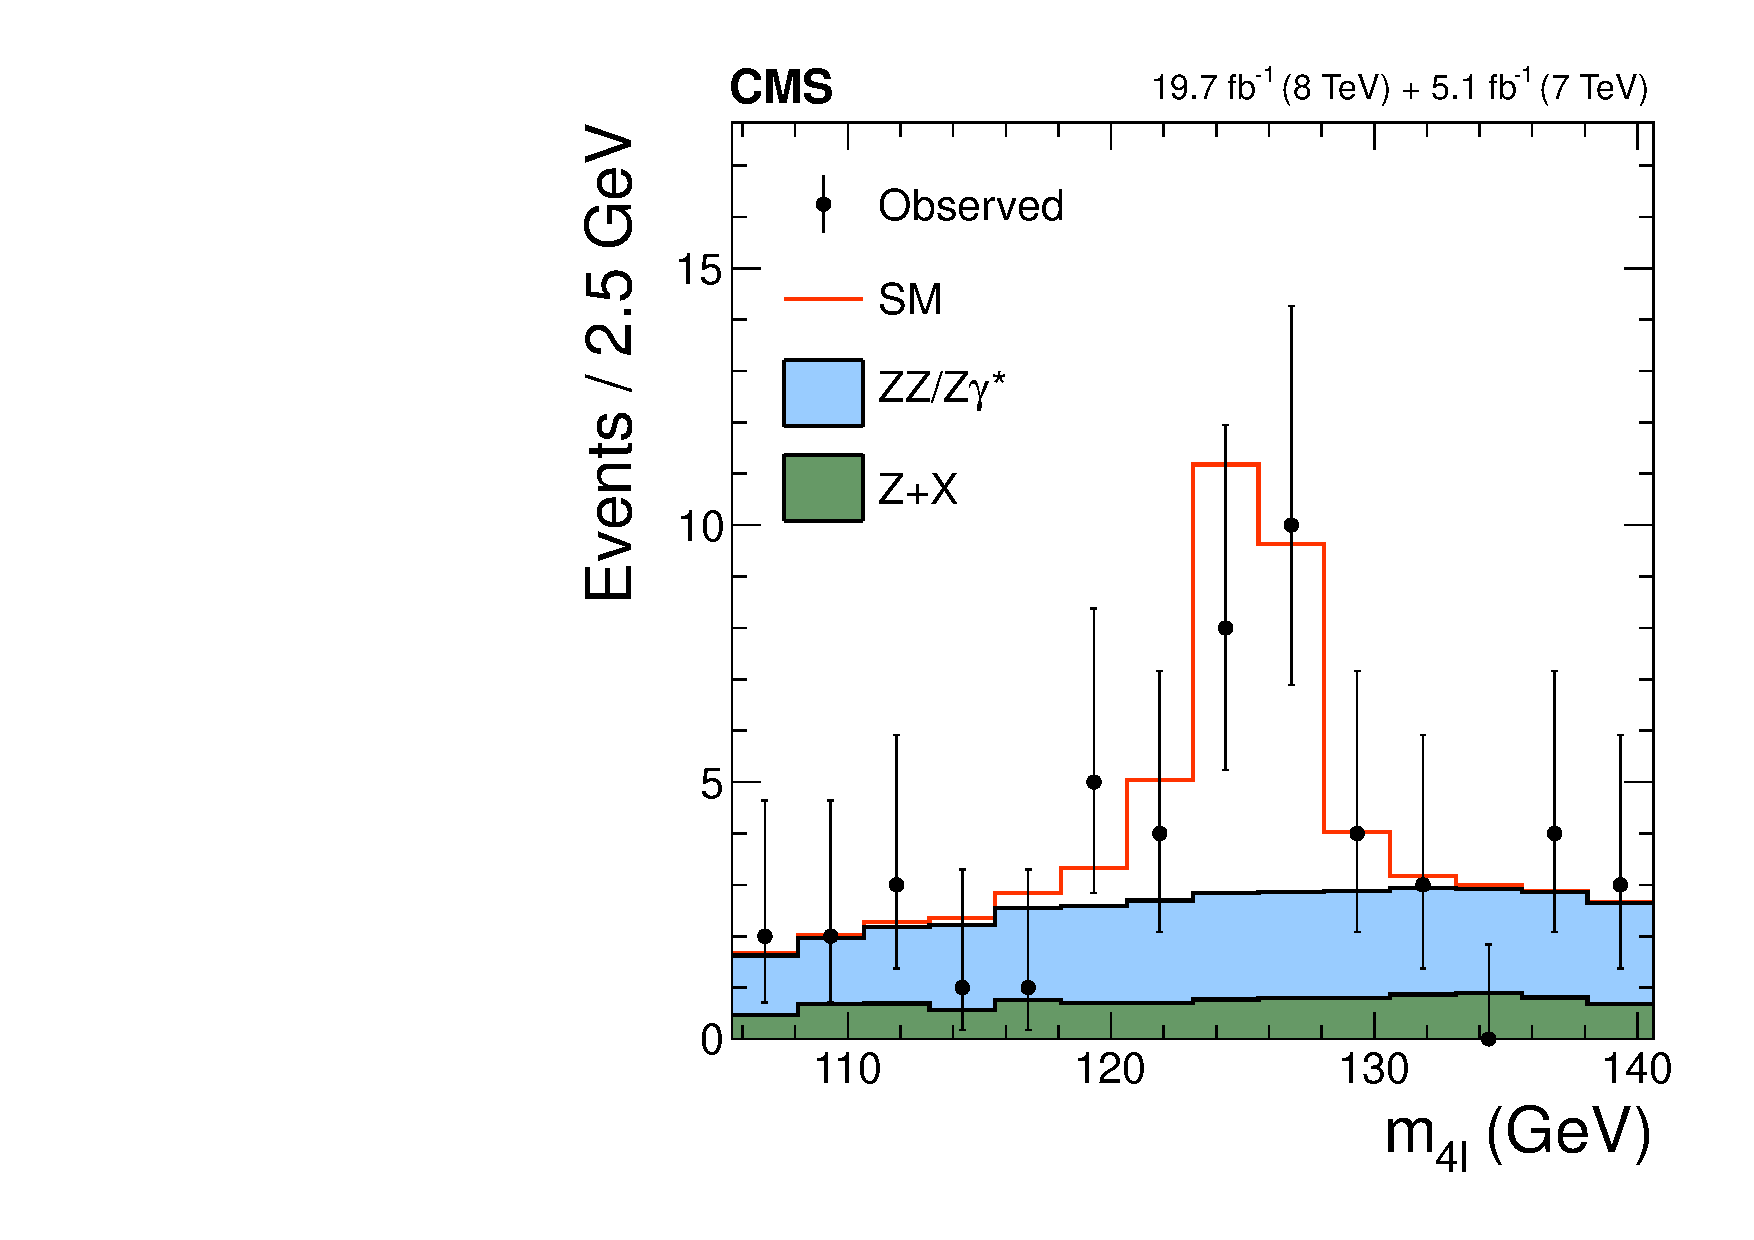
\includegraphics[width=0.32\textwidth]{Spin_Parity/cCompare_DataMC_AllTeV_ZZMass.pdf}
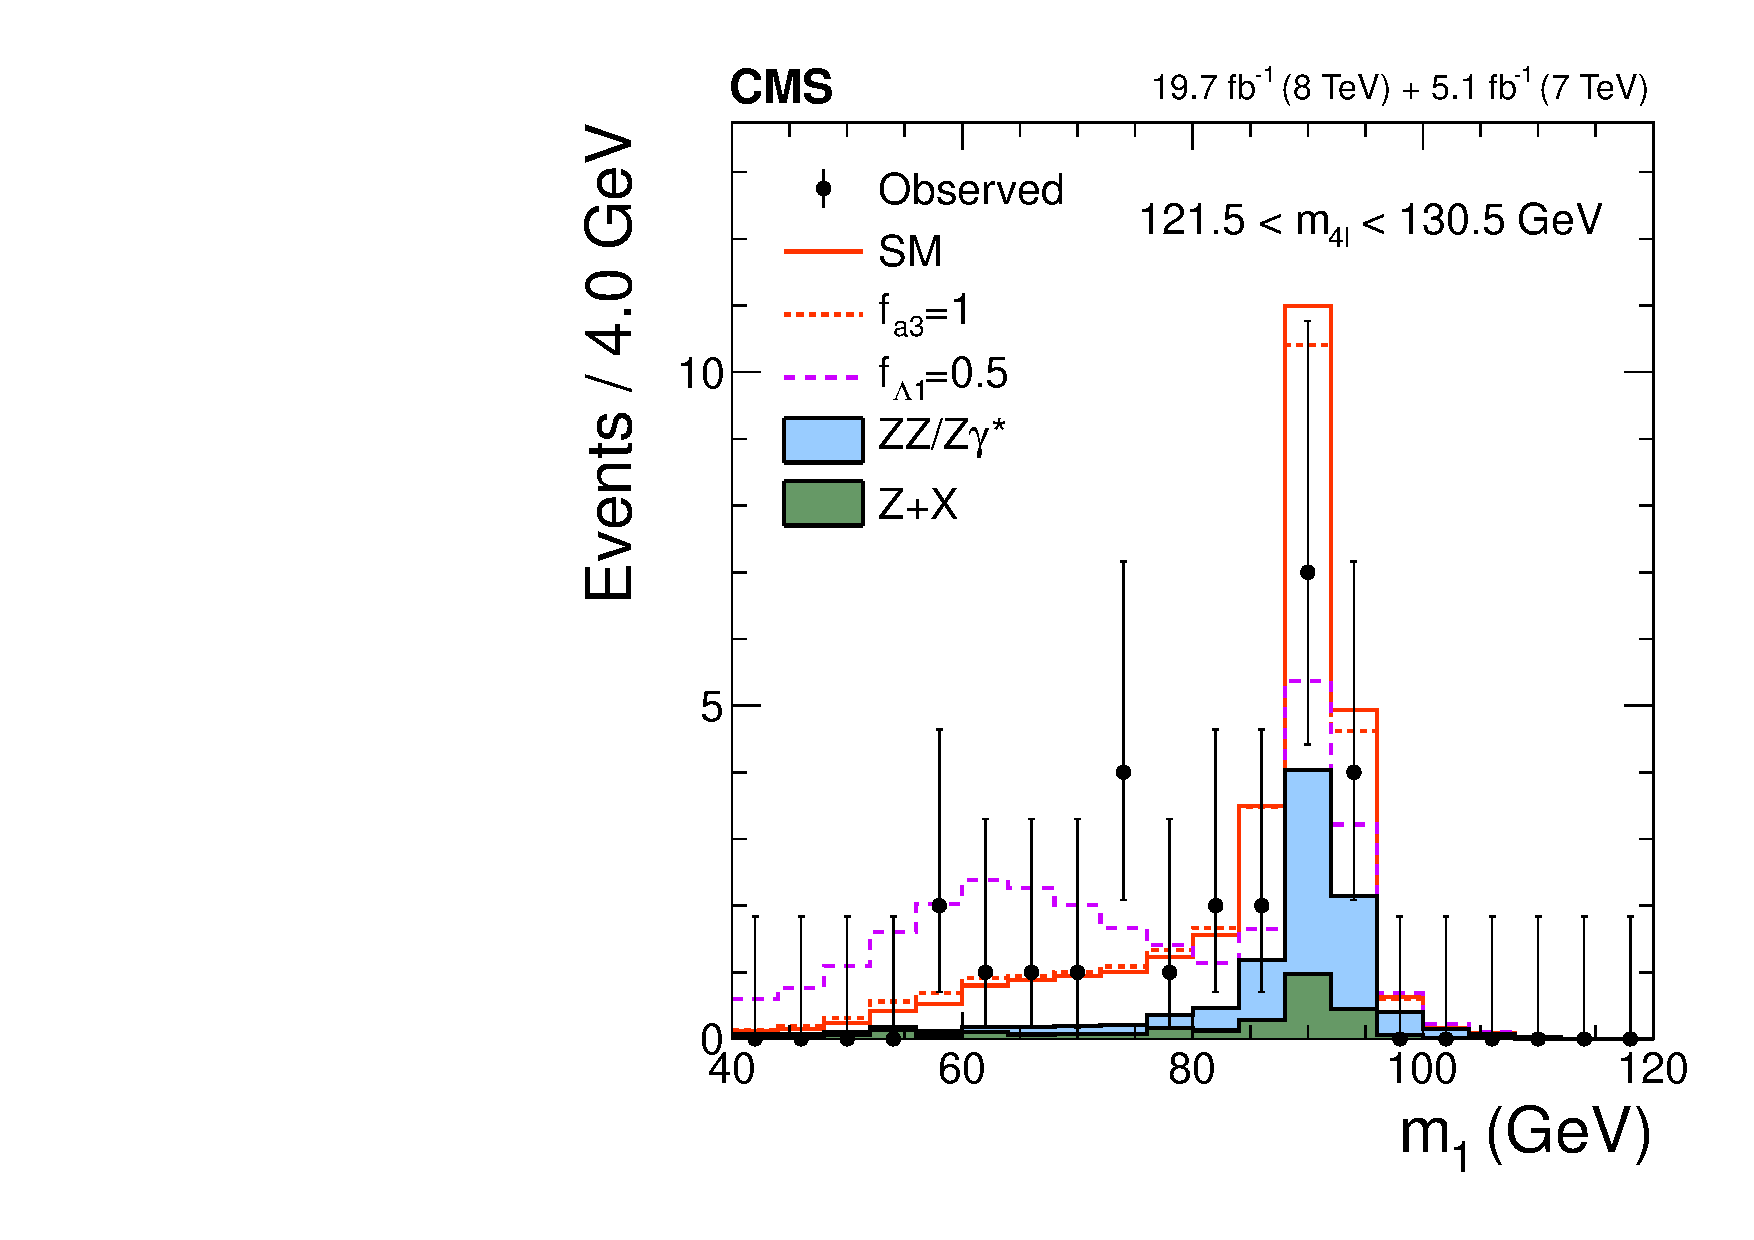
\includegraphics[width=0.32\textwidth]{Spin_Parity/cCompare_DataMC_AllTeV_Z1Mass_SignalEnriched.pdf}
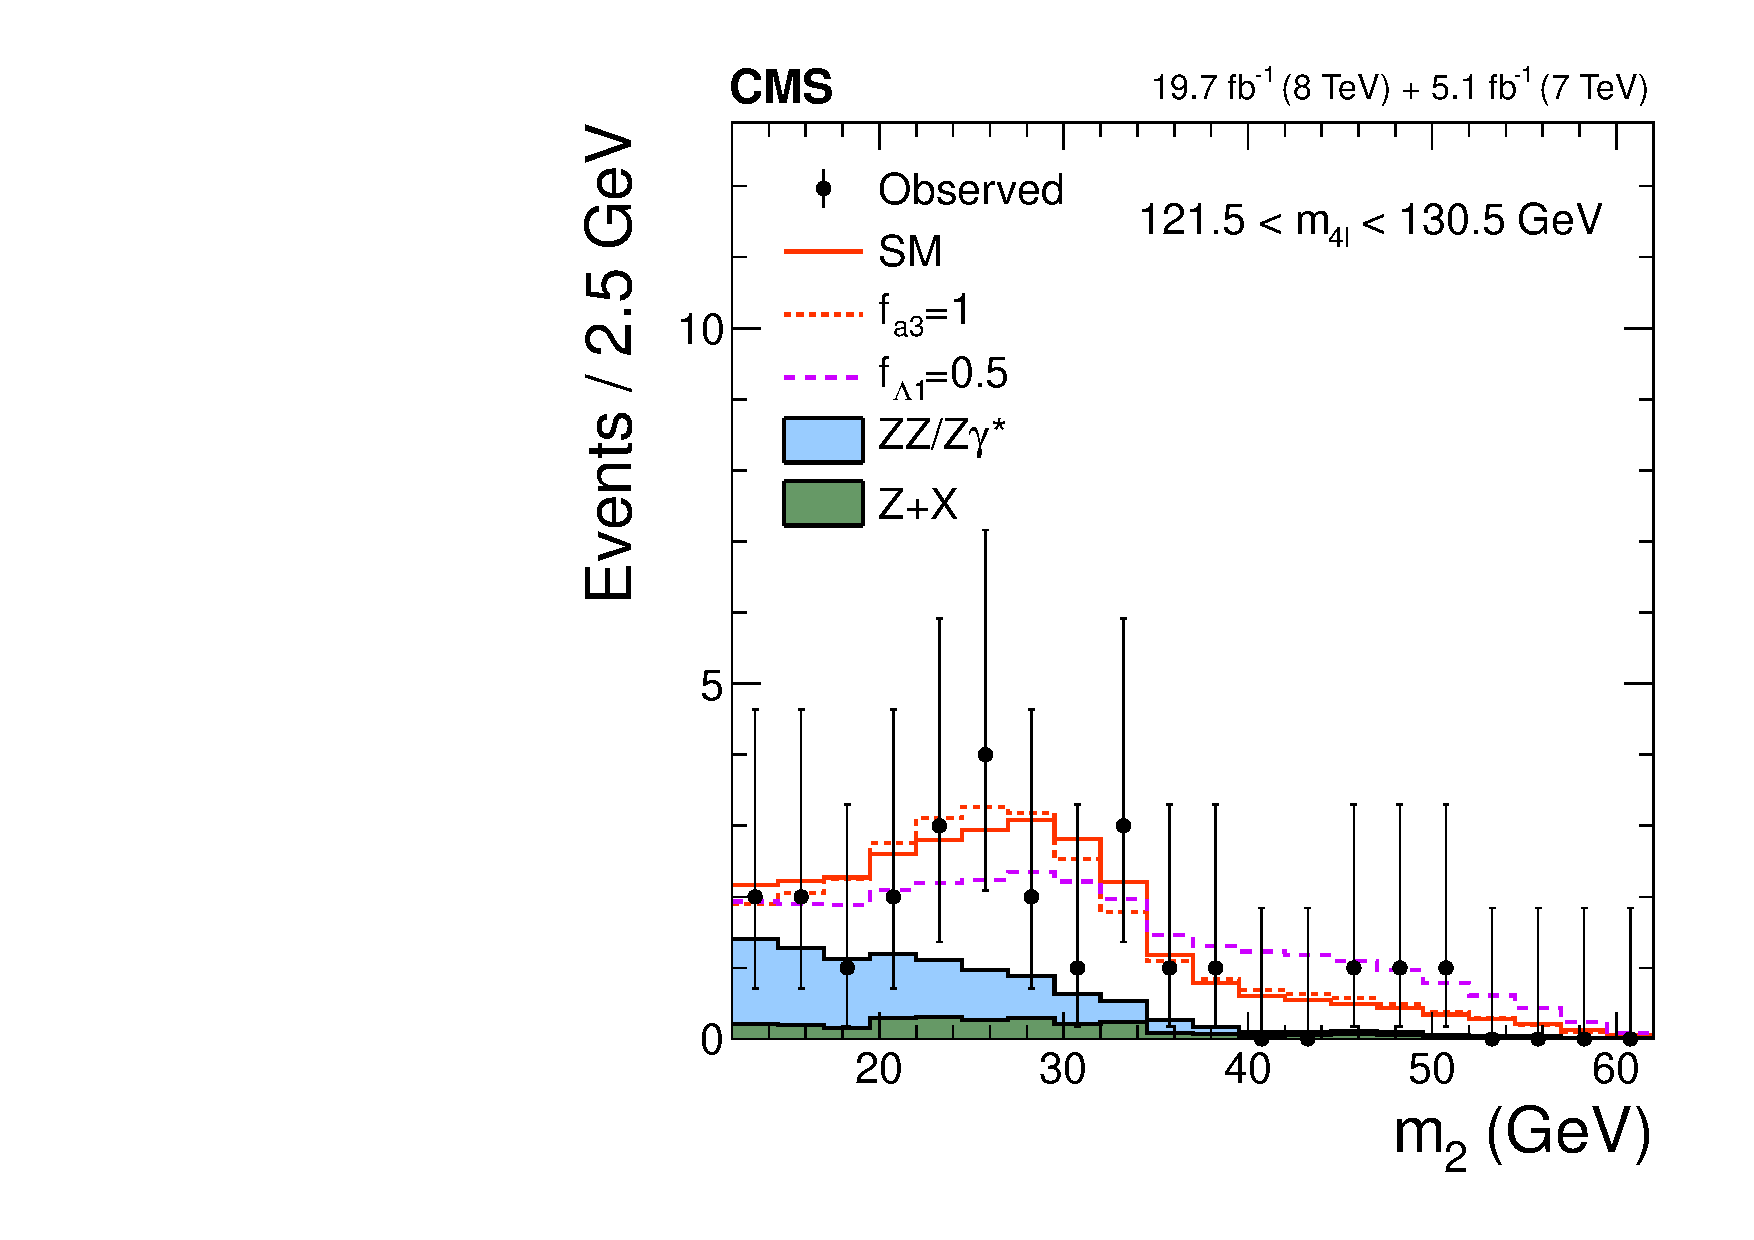
\includegraphics[width=0.32\textwidth]{Spin_Parity/cCompare_DataMC_AllTeV_Z2Mass_SignalEnriched.pdf} \\
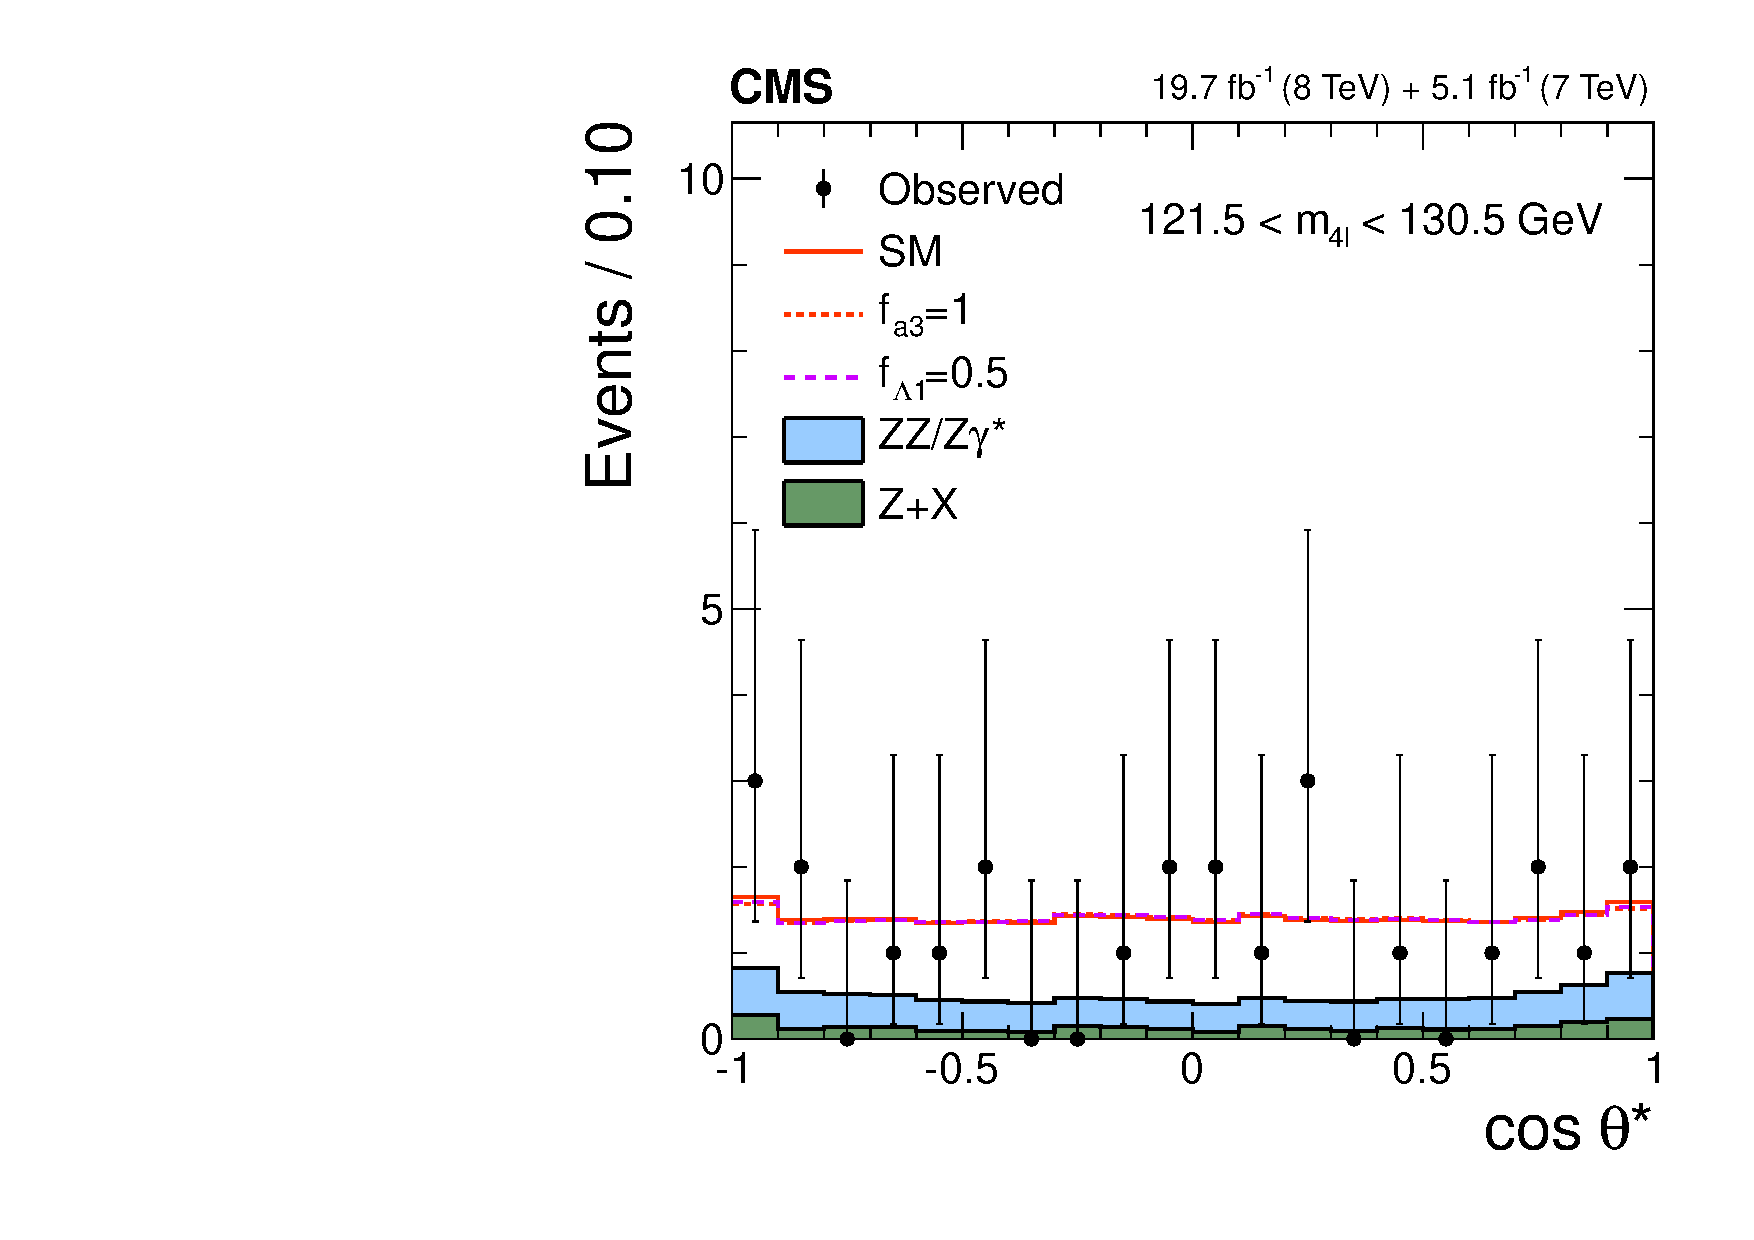
\includegraphics[width=0.32\textwidth]{Spin_Parity/cCompare_DataMC_AllTeV_costhetastar_SignalEnriched.pdf}
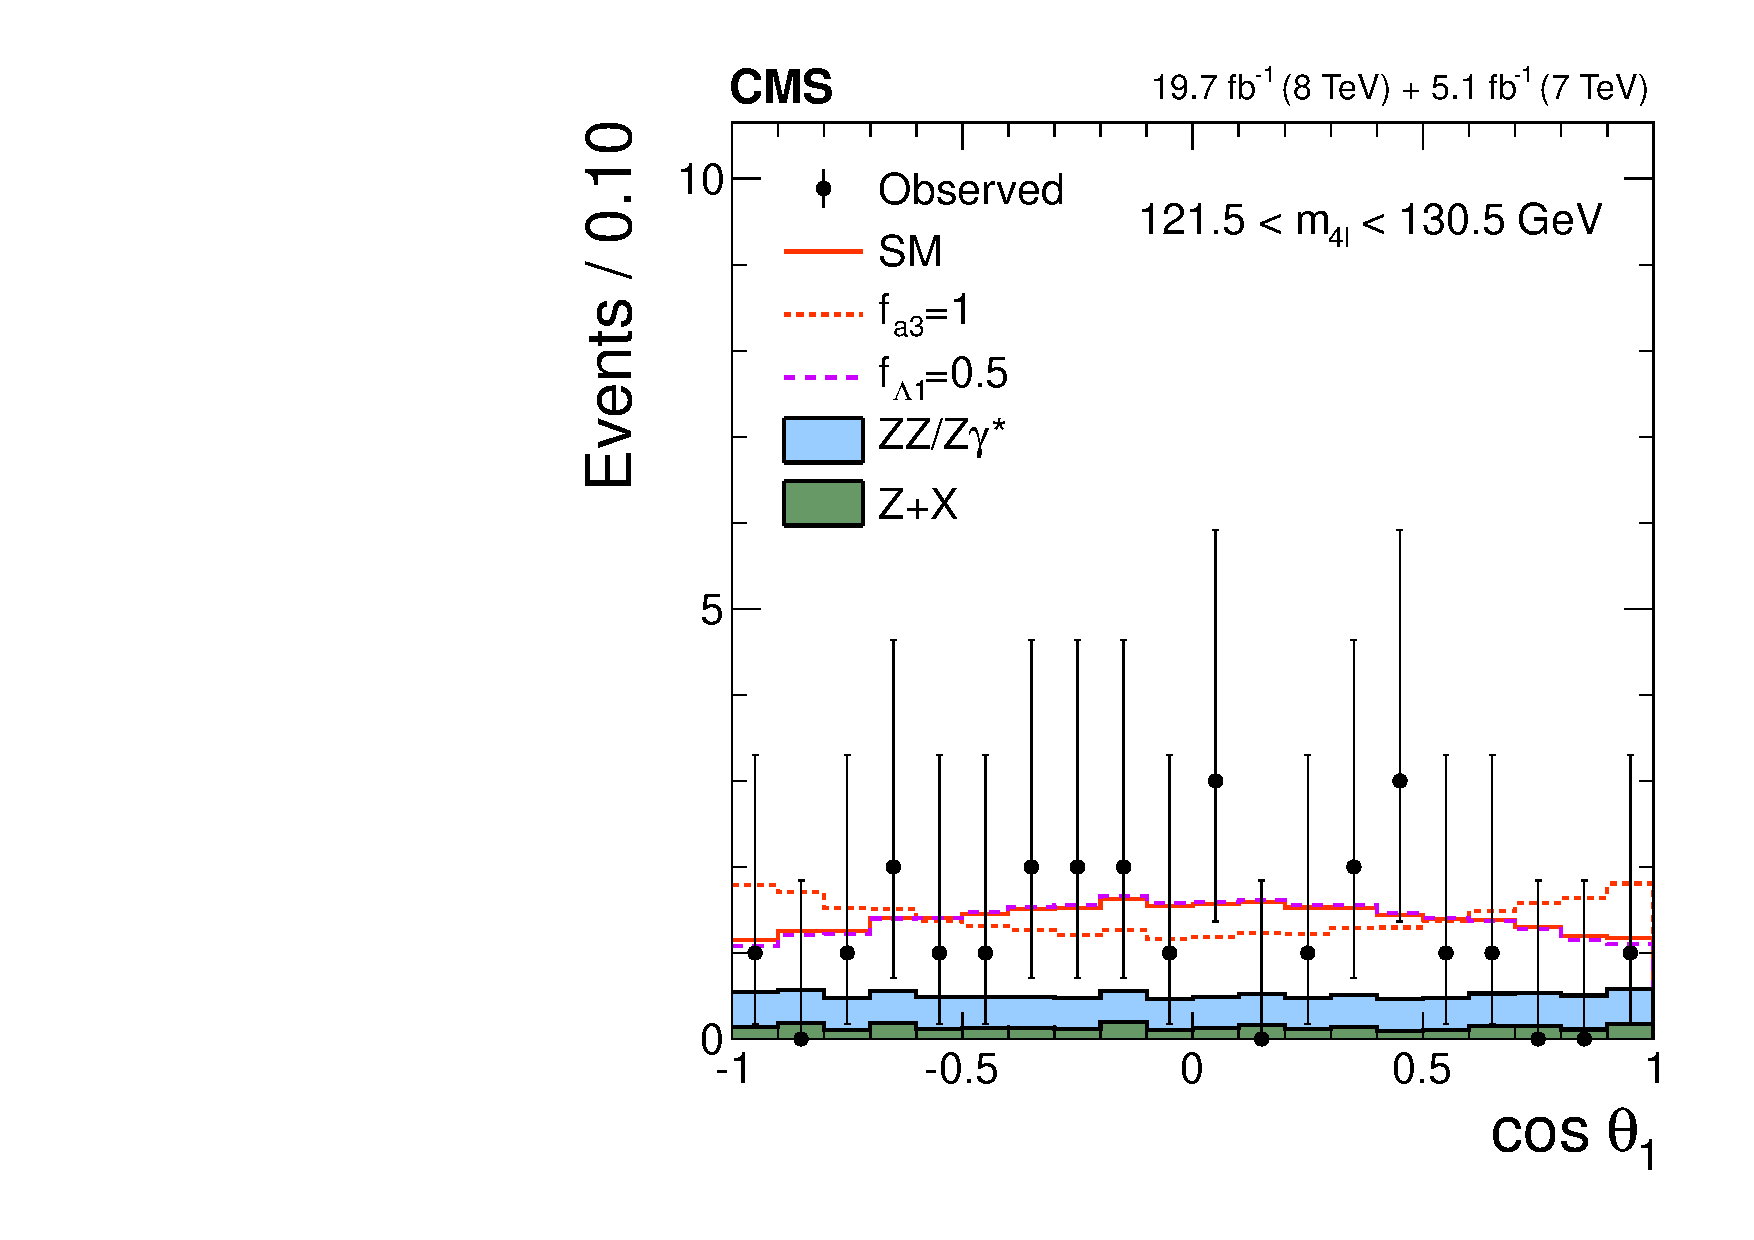
\includegraphics[width=0.32\textwidth]{Spin_Parity/cCompare_DataMC_AllTeV_helcosthetaZ1_SignalEnriched.pdf}
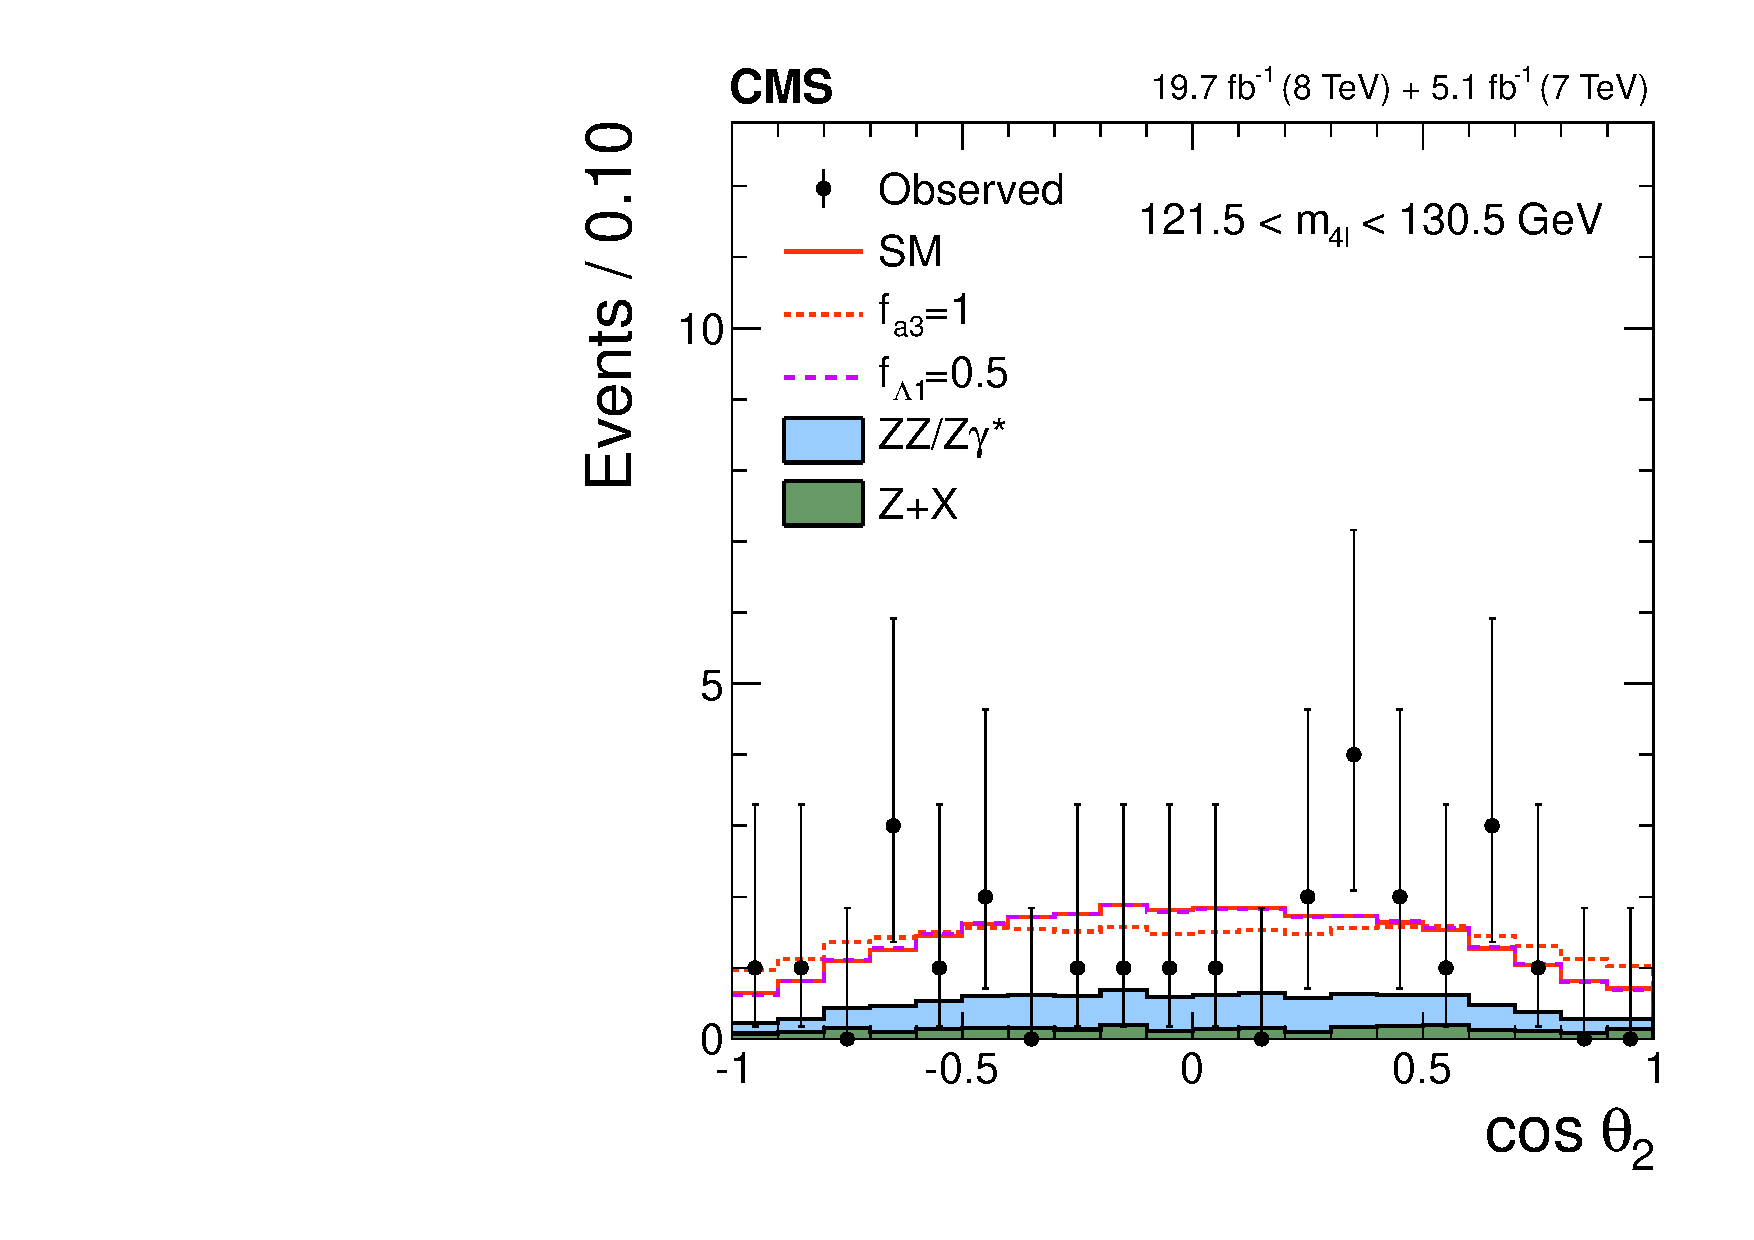
\includegraphics[width=0.32\textwidth]{Spin_Parity/cCompare_DataMC_AllTeV_helcosthetaZ2_SignalEnriched.pdf} \\
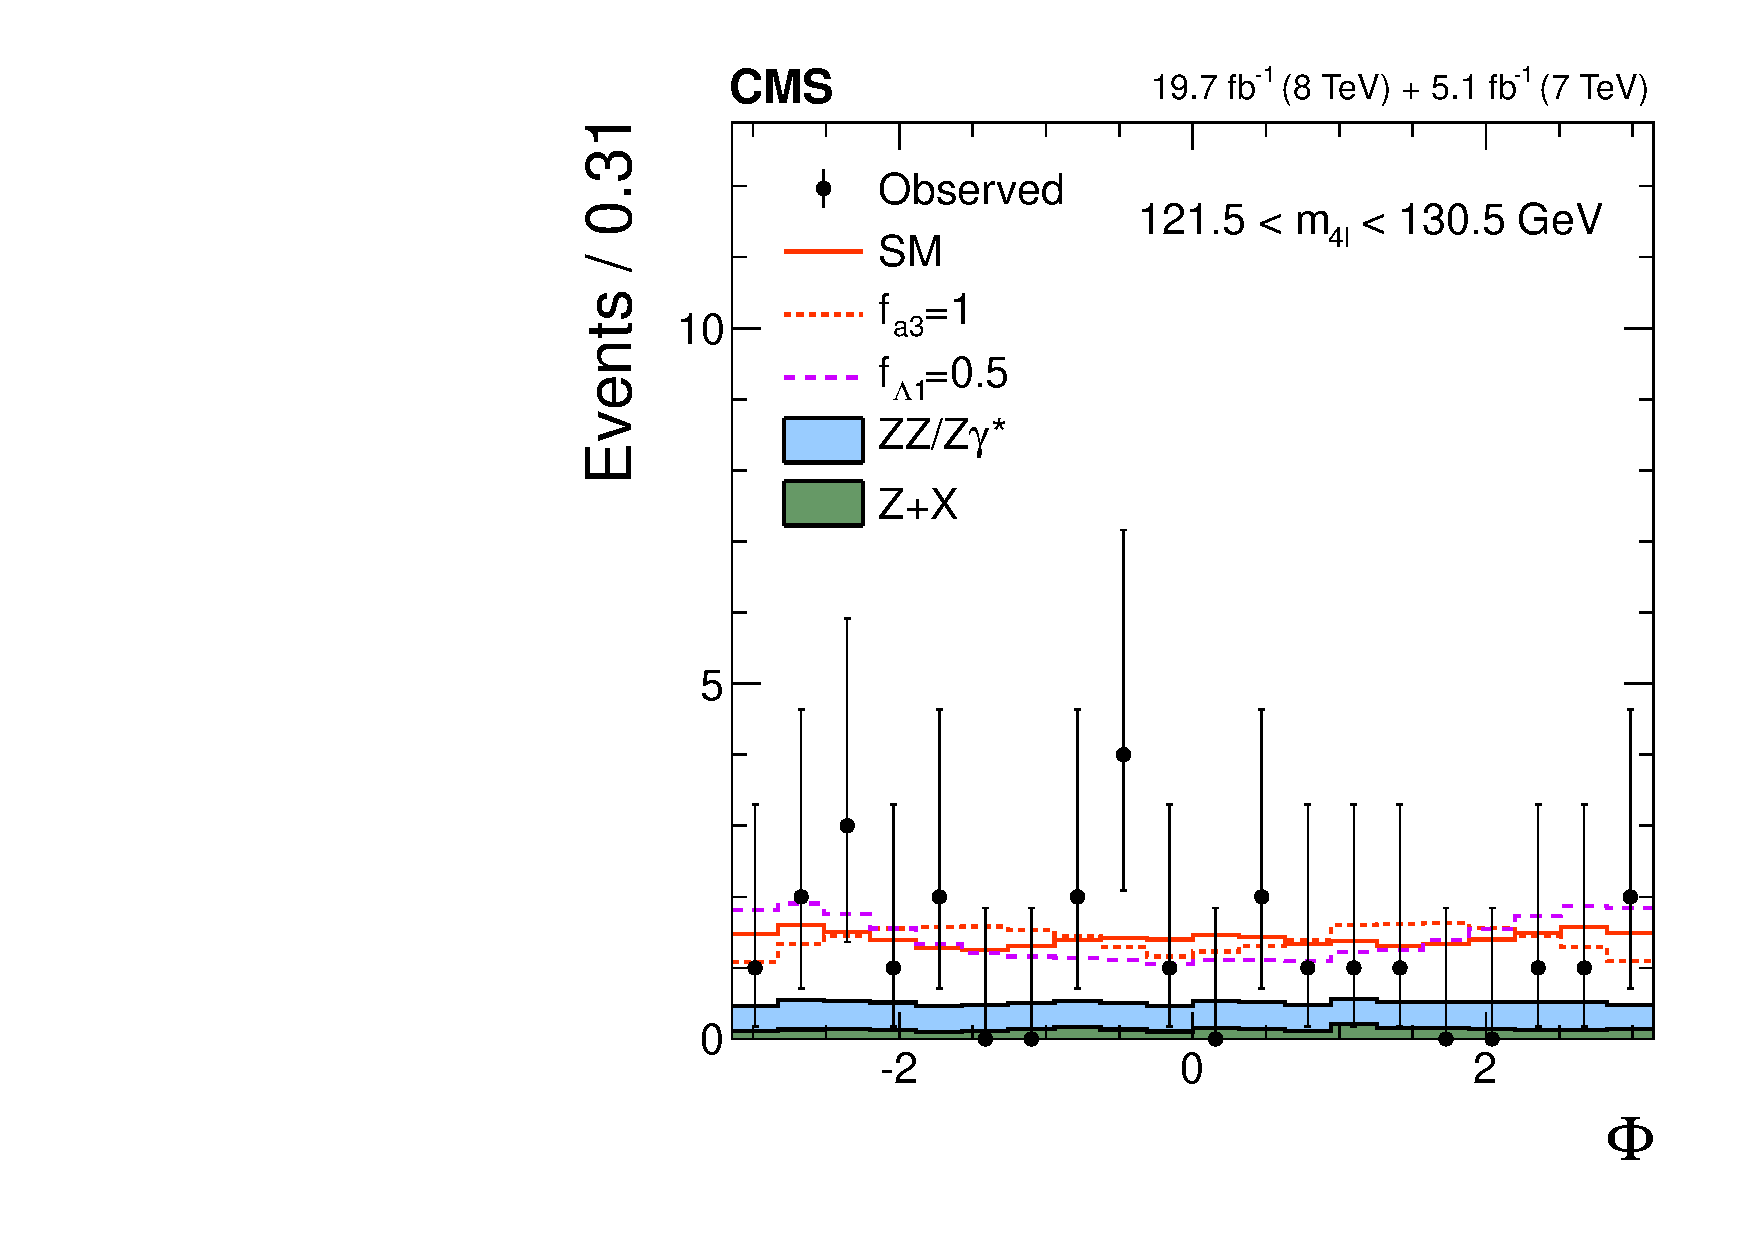
\includegraphics[width=0.32\textwidth]{Spin_Parity/cCompare_DataMC_AllTeV_helphi_SignalEnriched.pdf}
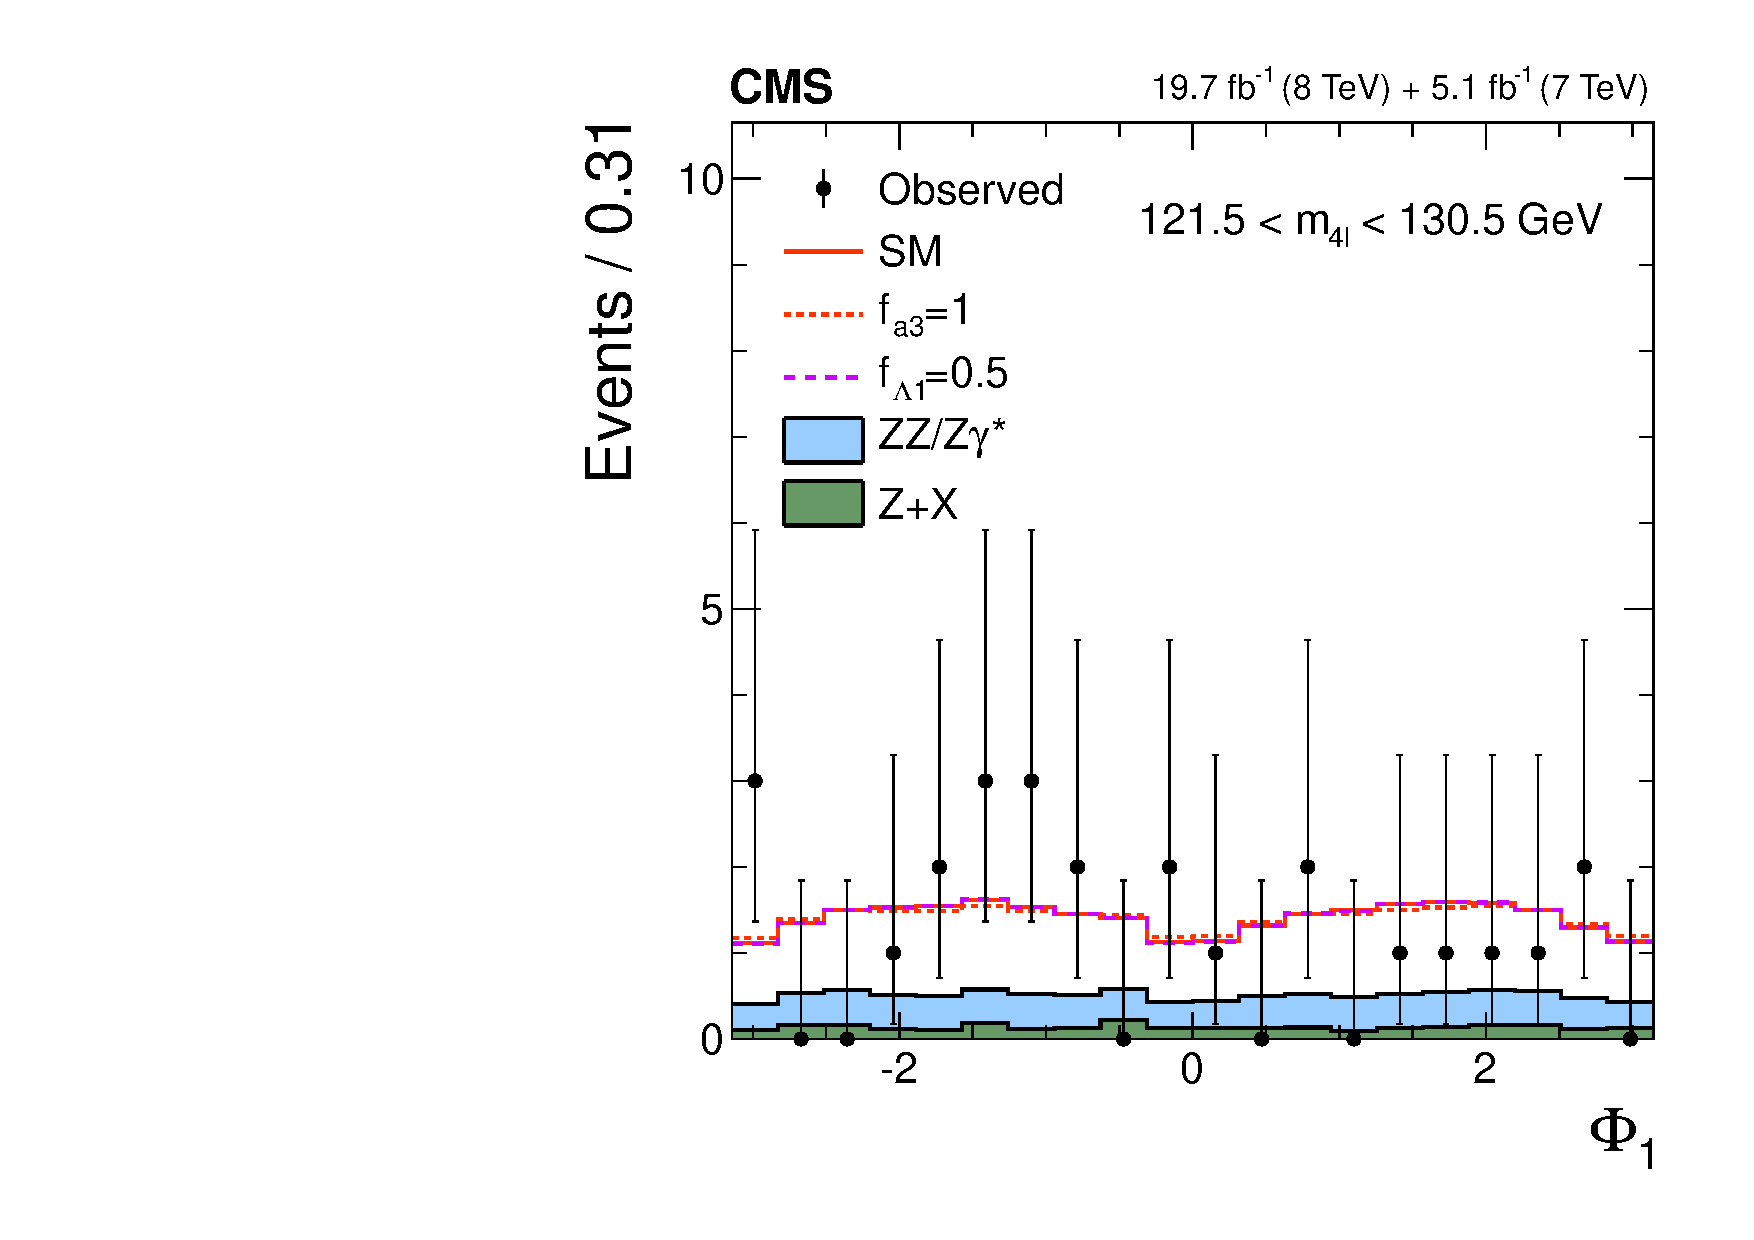
\includegraphics[width=0.32\textwidth]{Spin_Parity/cCompare_DataMC_AllTeV_phistarZ1_SignalEnriched.pdf}
\caption[Distributions of the eight kinematic observables used in the $H \to VV \to 4\ell$ analysis:
$m_{4\ell}$,
$m_1$,
$m_2$,
$\cos\theta^*$,
$\cos\theta_{1}$,
$\cos\theta_{2}$,
$\Phi$, and
$\Phi_{1}$.
The observed data (points with error bars), the expectations for the SM background (shaded areas),
the SM Higgs boson signal (open areas under the solid histogram),
and the alternative spin-zero resonances (open areas under the dashed histograms) are shown,
as indicated in the legend.
The mass of the resonance is taken to be $\unit{125.6}{\GeV}$ and the SM cross section is used.
All distributions, with the exception of $m_{4\ell}$, are presented with the requirement
$121.5 < m_{4\ell} < \unit{130.5}{\GeV}$.]{
Distributions of the eight kinematic observables used in the $H \to VV \to 4\ell$ analysis:
$m_{4\ell}$,
$m_1$,
$m_2$,
$\cos\theta^*$,
$\cos\theta_{1}$,
$\cos\theta_{2}$,
$\Phi$, and
$\Phi_{1}$.
The observed data (points with error bars), the expectations for the SM background (shaded areas),
the SM Higgs boson signal (open areas under the solid histogram),
and the alternative spin-zero resonances (open areas under the dashed histograms) are shown,
as indicated in the legend.
The mass of the resonance is taken to be $\unit{125.6}{\GeV}$ and the SM cross section is used.
All distributions, with the exception of $m_{4\ell}$, are presented with the requirement
$121.5 < m_{4\ell} < \unit{130.5}{\GeV}$ \cite{Khachatryan:2014kca}.
}
\label{fig:kinematics_sp}

\end{figure}

\subsection{MELA Observables} 
\label{sec:KDMethod}

A comprehensive analysis of the kinematics of the decay of a Higgs boson could include up to eight observables,
as discussed above. In such an analysis, it is required to have a parameterization of the multidimensional
distributions as a function of the parameters of interest. However, it becomes challenging to describe all
the correlations of the observables and detector effects. It is possible to reduce the number of observables
and keep the necessary information using the matrix element likelihood approach (MELA).
In this approach, the kinematic information is stored in a discriminant designed for the separation of
either background, the alternative signal components, or interference between those components.
The parameterization of up to three observables can be performed with full simulation or data from
the control regions.

The use of kinematic discriminants in Higgs boson studies was introduced in
previous CMS analyses~\cite{Chatrchyan:2012ufa,Chatrchyan:2012jja, Chatrchyan:2013mxa,Khachatryan:2014iha}
and feasibility studies~\cite{Bolognesi:2012mm,Anderson:2013afp},
and here it is extended both to a number of new models and to new techniques.
The construction of the kinematic discriminants follows the probabilities for an event are calculated using the LO matrix elements as a function
of angular and mass observables. In this way, the kinematic information, which fully characterizes
the $4\ell$ event topology of a certain process in its center-of-mass frame, is condensed to a
reduced number of observables.

The kinematic discriminants used in this study are computed using the \textsc{MELA}
package~\cite{Chatrchyan:2012ufa,Gao:2010qx,Bolognesi:2012mm,Anderson:2013afp},
which provides the full set of processes studied in this paper and uses \textsc{JHUGen} matrix elements
for the  signal,  $gg$ or $q\bar{q}\to X\to ZZ$ / $Z\gamma^*$ / $\gamma^*\gamma^*\to4\ell$,
and \textsc{MCFM} matrix elements for the background,
$gg$ or $q\bar{q}\to ZZ$ / $Z\gamma^*$ / $\gamma^*\gamma^*$ / $Z\to 4\ell$.
This library of processes is also consistent with the MC simulation used, and also includes other production and decay mechanisms.
Within the \textsc{MELA} framework, an analytic parameterization of the matrix elements
for signal~\cite{Gao:2010qx,Bolognesi:2012mm} and background~\cite{Chen:2012jy} was adopted in the previous CMS
analyses, reported in ~\cite{Chatrchyan:2012ufa,Chatrchyan:2013lba,Chatrchyan:2012jja}.
The above matrix element calculations are validated against each other and other methods for a subset of processes implemented in common.

Given several signal hypotheses defined for $gg$ or $q\bar{q}\to X\to ZZ$ / $Z\gamma^*$ / $\gamma^*\gamma^*\to4\ell$,
and the main background hypotheses $gg$ or $q\bar{q}\to ZZ$ / $Z\gamma^*$ / $\gamma^*\gamma^*$ / $Z\to 4\ell$,
the effective probabilities are defined for each event using a set of kinematic observables~$(m_1, m_2, m_{4\ell}, \vec\Omega)$
\begin{equation}\begin{aligned}
 \mathcal{P}_\mathrm{SM} =& \mathcal{P}^\text{kin}_\mathrm{SM} (m_1, m_2, \vec\Omega|m_{4\ell}) \times \mathcal{P}^\text{mass}_\text{sig} (m_{4\ell}|m_{H}), \\
 \mathcal{P}_{J^P} =& \mathcal{P}^\text{kin}_{J^P} (m_1, m_2, \vec\Omega|m_{4\ell}) \times \mathcal{P}^\text{mass}_\text{sig} (m_{4\ell}|m_{H}) ,\\
 \mathcal{P}_{J^P} ^\text{int} =& \left(\mathcal{P}^\text{kin}_\mathrm{SM + J^P}(m_1, m_2, \vec\Omega|m_{4\ell}) - \mathcal{P}^\text{kin}_{J^P} (m_1, m_2, \vec\Omega|m_{4\ell}) - \mathcal{P}^\text{kin}_\mathrm{SM}(m_1, m_2, \vec\Omega|m_{4\ell}) \right) , \\
 \mathcal{P}_{J^P} ^{\text{int} \perp} =& \left(\mathcal{P}^\text{kin}_{\mathrm{SM + J^P}\perp}(m_1, m_2, \vec\Omega|m_{4\ell}) - \mathcal{P}^\text{kin}_{J^P} (m_1, m_2, \vec\Omega|m_{4\ell}) - \mathcal{P}^\text{kin}_\mathrm{SM}(m_1, m_2, \vec\Omega|m_{4\ell}) \right) , \\
 \mathcal{P}_{q\bar{q}ZZ} =& \mathcal{P}^\text{kin}_{q\bar{q}ZZ} (m_1, m_2, \vec\Omega|m_{4\ell}) \times \mathcal{P}^\text{mass}_{q\bar{q}ZZ} (m_{4\ell}) , \\
 \mathcal{P}_{ggZZ} =& \mathcal{P}^\text{kin}_{ggZZ} (m_1, m_2, \vec\Omega|m_{4\ell}) \times \mathcal{P}^\text{mass}_{ggZZ} (m_{4\ell}) ,
\label{eq:kd-prob-gg}
\end{aligned}\end{equation}

where $\mathcal{P}^\text{kin}(m_1, m_2, \vec\Omega|m_{H}) = |{A}(m_1, m_2, \vec\Omega|m_{H})|^2$
are the probabilities computed from the LO matrix elements and generally are not normalized.
The variable $\mathcal{P}^\text{mass}(m_{4\ell}|m_{H})$ is the probability as a function of the four-lepton reconstructed mass
and is calculated using the $m_{4\ell}$ parameterization described in previously in section \ref{sec:4l_Experiment}
including the $m_{H}=\unit{125.6}{\GeV}$ hypothesis for signal.
The probabilities $\mathcal{P}_{J^P} ^\text{int}$ parameterize interference between contributions from the SM and
anomalous couplings, where $J^P$ refers to a spin-zero tensor structure of interest, and are allowed to have both positive
and negative values. In the calculation of the mixed amplitude used for $\mathcal{P}^\text{kin}_\mathrm{SM + J^P}$,
the same coupling strengths are used as in the individual probabilities $\mathcal{P}^\text{kin}_\mathrm{SM}$ and $\mathcal{P}^\text{kin}_{J^P}$,
and these couplings are required to provide equal cross sections for the two individual processes.
The quantity $\mathcal{P}_{J^P} ^{\text{int}\perp}$ is constructed in the same way
as $\mathcal{P}_{J^P} ^\text{int}$ except that the phase of the $J^P$ amplitude is changed by $\pi/2$.
The matrix element calculations in equation \eqref{eq:kd-prob-gg} are also used for the re-weighting of simulated samples.

Several kinematic discriminants are constructed for the main signal and background processes
from the set of probabilities described above
\begin{equation}\begin{aligned}
 \mathcal{D}_\text{bkg} =& \frac{\mathcal{P}_\mathrm{SM} }{\mathcal{P}_\mathrm{SM} +\mathcal{P}_{q\bar{q}ZZ} }=
\left[1+\frac{\mathcal{P}^\text{kin}_{q\bar{q}ZZ} (m_1, m_2, \vec\Omega | m_{4\ell})\times \mathcal{P}^\text{mass}_{q\bar{q}ZZ} (m_{4\ell})  }
{\mathcal{P}^\text{kin}_\mathrm{SM} (m_1, m_2, \vec\Omega | m_{4\ell}) \times \mathcal{P}^\text{mass}_\text{sig} (m_{4\ell}|m_{H}) } \right]^{-1} ,
 \\
\mathcal{D}_{J^P} =& \frac{\mathcal{P}_\mathrm{SM} }{\mathcal{P}_\mathrm{SM} + \mathcal{P}_{J^P} }=
\left[1+ \frac{\mathcal{P}^\text{kin}_{J^P} (m_1, m_2, \vec\Omega | m_{4\ell}) }
{\mathcal{P}^\text{kin}_\mathrm{SM} (m_1, m_2, \vec\Omega | m_{4\ell}) } \right]^{-1} ,
 \\
\mathcal{D}_\text{int} =& \frac{ \mathcal{P}_{J^P}^\text{int}(m_1, m_2, \vec\Omega | m_{4\ell})}
{\mathcal{P}^\text{kin}_\mathrm{SM} +\mathcal{P}^\text{kin}_{J^P} }  .
\end{aligned}\end{equation}

The observable $\mathcal{D}_\text{bkg}$ is used to separate signal from $q\bar{q} \to ZZ$, $gg \to ZZ$, and $Z+\text{jets}$ backgrounds,
using the $m_{4\ell}$ probability in addition to $\mathcal{P}^\text{kin}$. The discriminant $\mathcal{D}_{J^P}$ is created to separate
the SM signal from an alternative $J^P$ state. The discriminant $\mathcal{D}_\text{int}$ is created to isolate interference between
the SM and anomalous coupling contributions. Since the analysis is designed to probe small anomalous couplings, interference
between different anomalous contributions is a negligible effect and dedicated discriminants for those contributions are not
considered. The variable $\mathcal{D}_\text{int}$ is denoted as $\mathcal{D}_{C\!P}$ for interference between the $a_{1}$ and $a_{3}$ contributions
because it is sensitive to $CP$ violation~\cite{Anderson:2013afp}.


To remove the dependence of the spin-one and spin-two discriminants on the production model,
the probability $\mathcal{P}^\text{kin}$ is averaged over the two production angles $\cos\theta^*$ and $\Phi_1$,
defined in figure~\ref{fig:decay}, or equivalently the signal matrix element squared is averaged over the
polarization of the resonance~\cite{Anderson:2013afp}. The production independent discriminants
are defined as
\begin{equation}\begin{aligned}
\label{eq:melaSigProd}
\mathcal{D}^\text{dec}_\text{bkg} =&
\Bigg[1+\frac{\frac{1}{4\pi}\int \mathrm{d}\Phi_1  \mathrm{d}\cos\theta^{*}
\mathcal{P}^\text{kin}_{q\bar{q}ZZ} (m_1, m_2, \vec\Omega | m_{4\ell})\times \mathcal{P}^\text{mass}_{q\bar{q}ZZ} (m_{4\ell})  }
{\mathcal{P}^\text{kin}_\mathrm{SM} (m_1, m_2, \vec\Omega | m_{4\ell}) \times \mathcal{P}^\text{mass}_\text{sig} (m_{4\ell}|m_{H}) } \Bigg]^{-1} ,
 \\
\mathcal{D}^\text{dec}_{J^P} =&
\left[1+\frac{\frac{1}{4\pi}\int \mathrm{d}\Phi_1  \mathrm{d}\cos\theta^{*}
\mathcal{P}^\text{kin}_{J^P} (m_1, m_2, \vec\Omega | m_{4\ell}) }
{\mathcal{P}^\text{kin}_\mathrm{SM} (m_1, m_2, \vec\Omega | m_{4\ell}) } \right]^{-1} .
\end{aligned}\end{equation}
The decay kinematics of a spin-zero resonance are already independent of the production
mechanism, due to the lack of spin correlations for any spin-zero particle.
The small differences in the distributions of the production-independent discriminants
with the different production mechanisms are due to detector acceptance effects
and are treated as systematic uncertainties.

A complete list of all the discriminants used in the analysis is presented in table~\ref{tab:kdlist}.
Some examples of the distributions as expected from simulation and as observed in data can be seen
in figure~\ref{fig:discriminants} for all the discriminants used in the study of the spin-zero $HZZ$ couplings.
A complete list of the measurements performed and observables used is discussed in sections~\ref{sec:ResultsExotic}
and~\ref{sec:ResultsSpinZero}. 

From figure \ref{fig:discriminants} the special role of $\mathcal{D}_{C\!P}$ can be observed. For the SM background processes, including a SM Higgs boson, this distribution is completely symmetric. However, if the observed boson contains a $C\!P$-violating component it will appear as an asymmetry in this distribution as shown by the $f_{a3} = 0.5$ example in the figure. 

\begin{table}
\centering
\caption[List of observables $\vec{x}$ used in the analysis of the $HVV$ couplings.
The $J^P$ notation for spin-two refers to the ten scenarios defined in table~\ref{tab:scenarios}.
]{
List of observables $\vec{x}$ used in the analysis of the $HVV$ couplings.
The $J^P$ notation for spin-two refers to the ten scenarios defined in table~\ref{tab:scenarios} \cite{Khachatryan:2014kca}.
}
\label{tab:kdlist}
\begin{tabular}{cccc}
 Measurement  & \multicolumn{3}{c}{Observables $\vec{x}$} \\
\hline
 $f_{\Lambda1}$ & $\mathcal{D}_\text{bkg}$ & $\mathcal{D}_{\Lambda1}$ & \\
 $f_{a2}$ &  $\mathcal{D}_\text{bkg}$ & $\mathcal{D}_{0h+}$ & $\mathcal{D}_\text{int}$ \\
  $f_{a3}$ &  $\mathcal{D}_\text{bkg}$ & $\mathcal{D}_{0-}$ & $\mathcal{D}_{C\!P}$ \\
  $f_{\Lambda1}^{Z\gamma}$ &  $\mathcal{D}_\text{bkg}$ & $\mathcal{D}^{Z\gamma}_{\Lambda1}$  & $\mathcal{D}^{Z\gamma,\Lambda1}_\text{int}$  \\
  $f_{a2}^{Z\gamma}$ &  $\mathcal{D}_\text{bkg}$ & $\mathcal{D}^{Z\gamma}_{a2}$  & $\mathcal{D}_\text{int}^{Z\gamma}$ \\
  $f_{a3}^{Z\gamma}$ &  $\mathcal{D}_\text{bkg}$ & $\mathcal{D}^{Z\gamma}_{a3}$  & $\mathcal{D}_{C\!P}^{Z\gamma}$ \\
 $f_{a2}^{\gamma\gamma}$  &  $\mathcal{D}_\text{bkg}$ & $\mathcal{D}^{\gamma\gamma}_{a2}$  & $\mathcal{D}_\text{int}^{\gamma\gamma}$ \\
  $f_{a3}^{\gamma\gamma}$ & $\mathcal{D}_\text{bkg}$ & $\mathcal{D}^{\gamma\gamma}_{a3}$ & $\mathcal{D}_{C\!P}^{\gamma\gamma}$ \\
 \multicolumn{1}{l}{spin-one $q\bar{q}\to X (f_{b2})\to ZZ$} &  $\mathcal{D}_\text{bkg}$ & $\mathcal{D}_{1-}$ & $\mathcal{D}_{1+}$ \\

 \multicolumn{1}{l}{spin-one decay  $X(f_{b2})\to ZZ$} &  $\mathcal{D}_\text{bkg}^\text{dec}$ & $\mathcal{D}_{1-}^\text{dec}$ & $\mathcal{D}_{1+}^\text{dec}$ \\
 \multicolumn{1}{l}{spin-two $q\bar{q}\to X (J^P)\to ZZ$} &  $\mathcal{D}_\text{bkg}$ & $\mathcal{D}_{J^P}^{q\bar{q}}$ & \\

 \multicolumn{1}{l}{spin-two $gg\to X (J^P)\to ZZ$} &  $\mathcal{D}_\text{bkg}$ & $\mathcal{D}_{J^P}^{gg}$ & \\

 \multicolumn{1}{l}{spin-two decay $X (J^P)\to ZZ$}&  $\mathcal{D}_\text{bkg}^\text{dec}$ & $\mathcal{D}_{J^P}^\text{dec}$ & \\
\end{tabular}

\end{table}

\begin{figure}
\centering
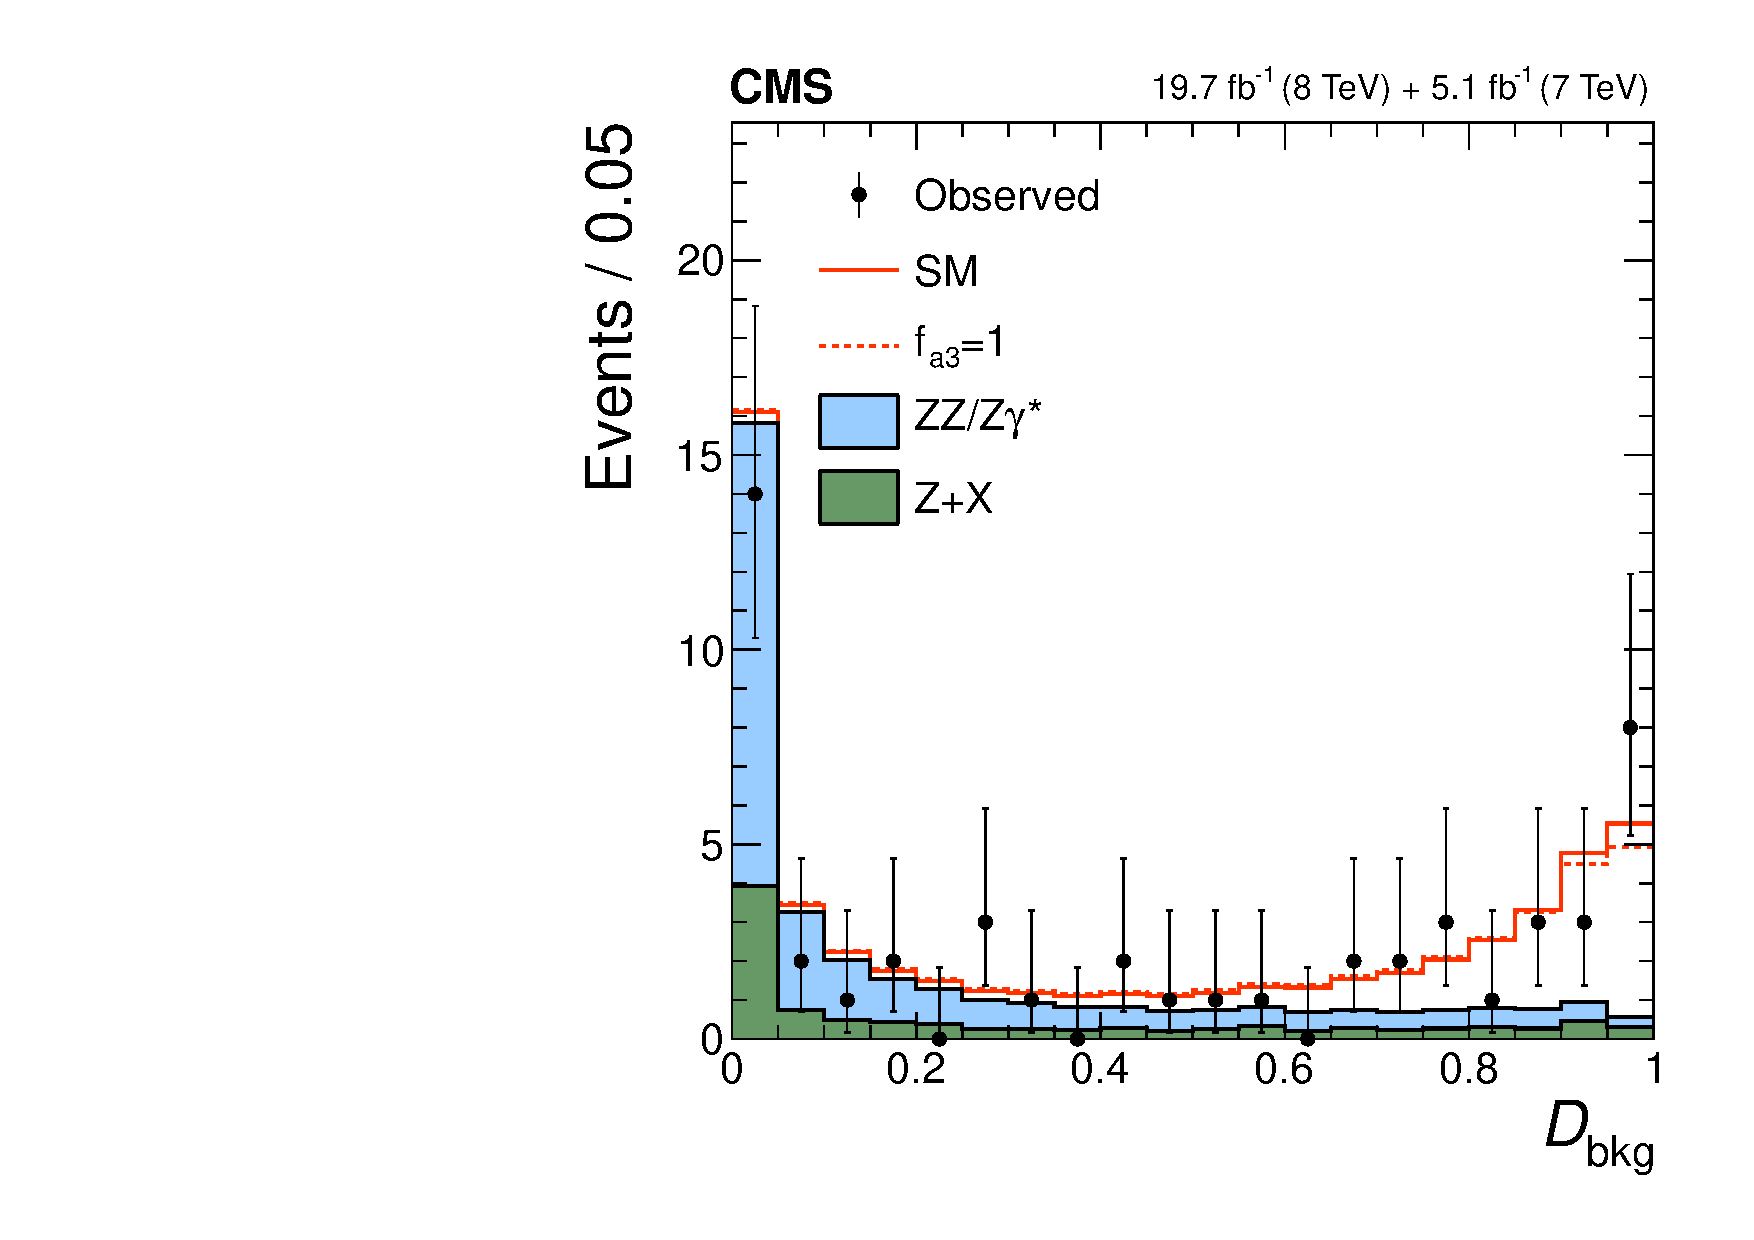
\includegraphics[width=0.32\textwidth]{Spin_Parity/cCompare_DataMC_AllTeV_D_bkg.pdf}
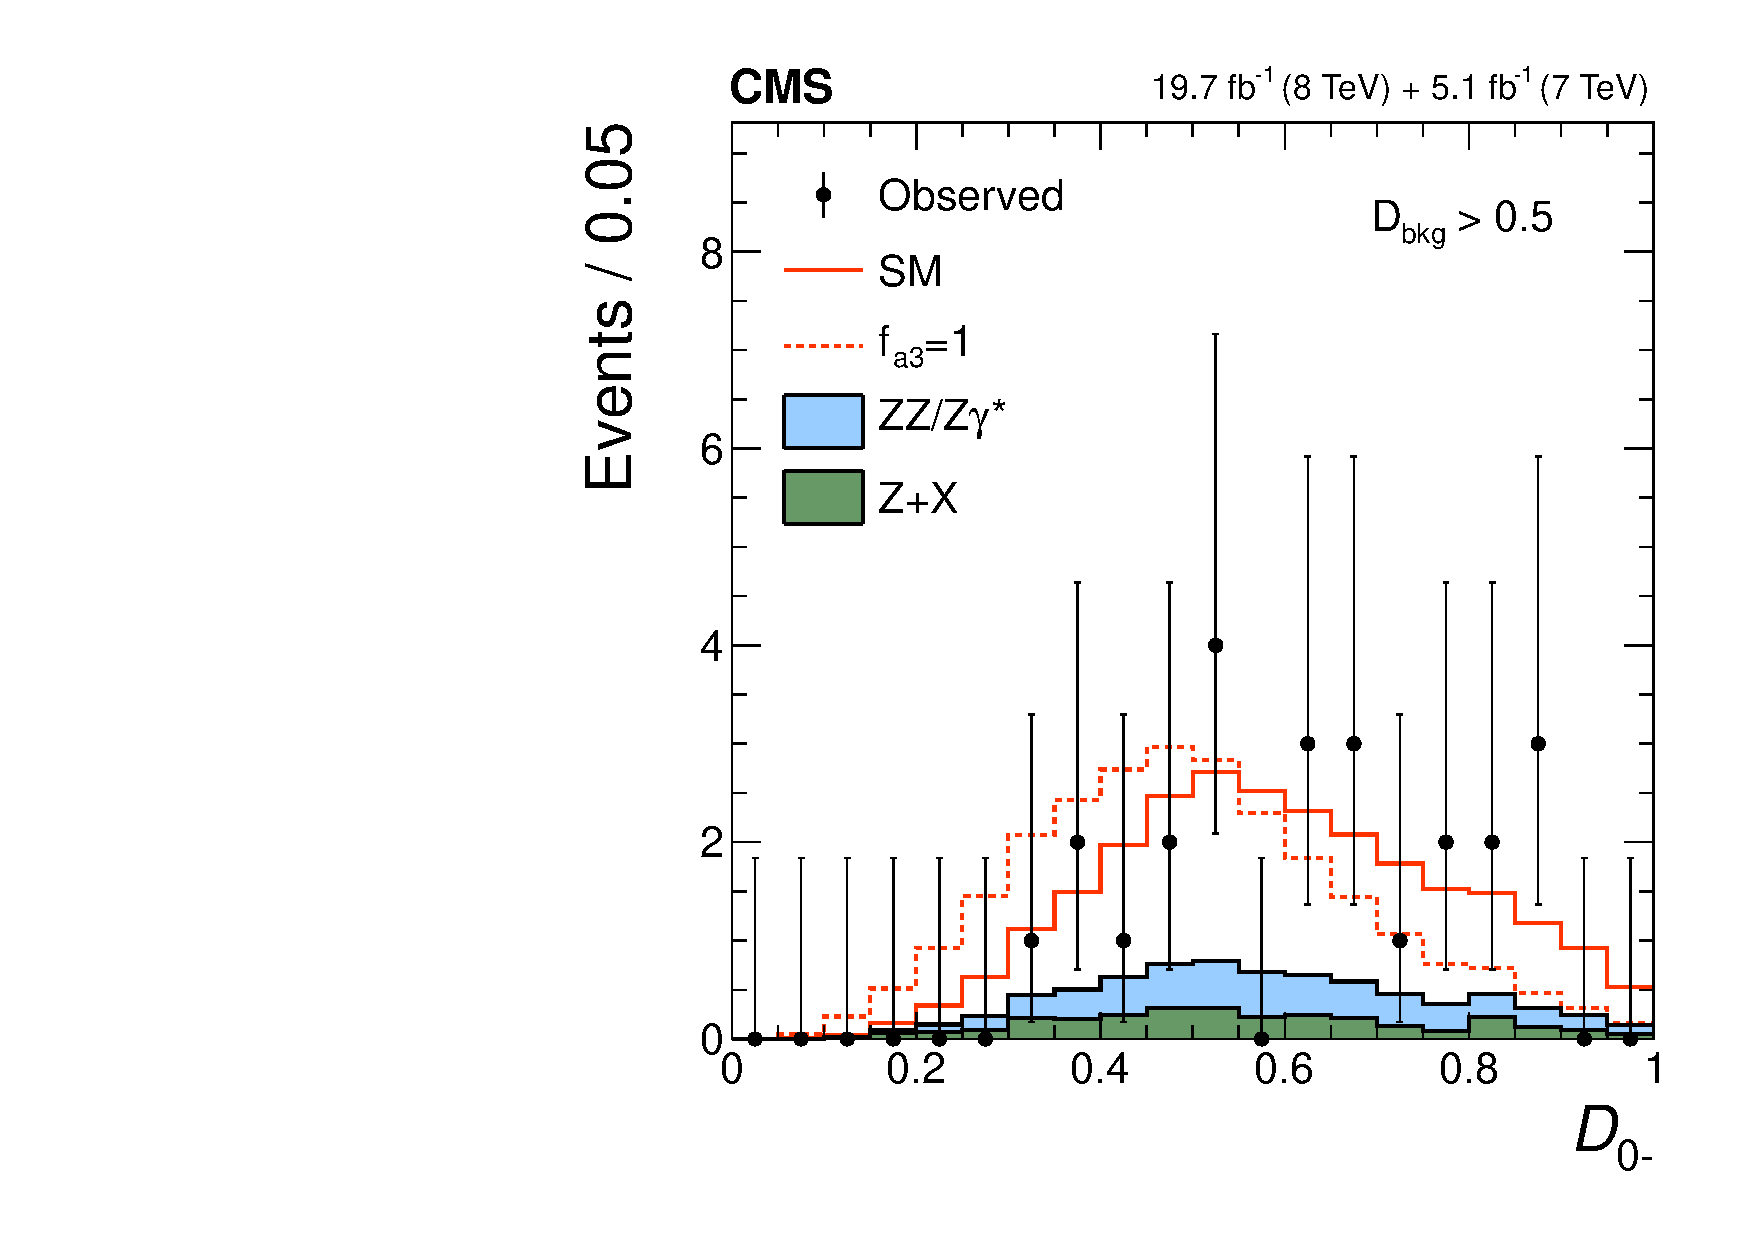
\includegraphics[width=0.32\textwidth]{Spin_Parity/cCompare_DataMC_AllTeV_D_g1_vs_g4_phi0_SignalEnriched.pdf}
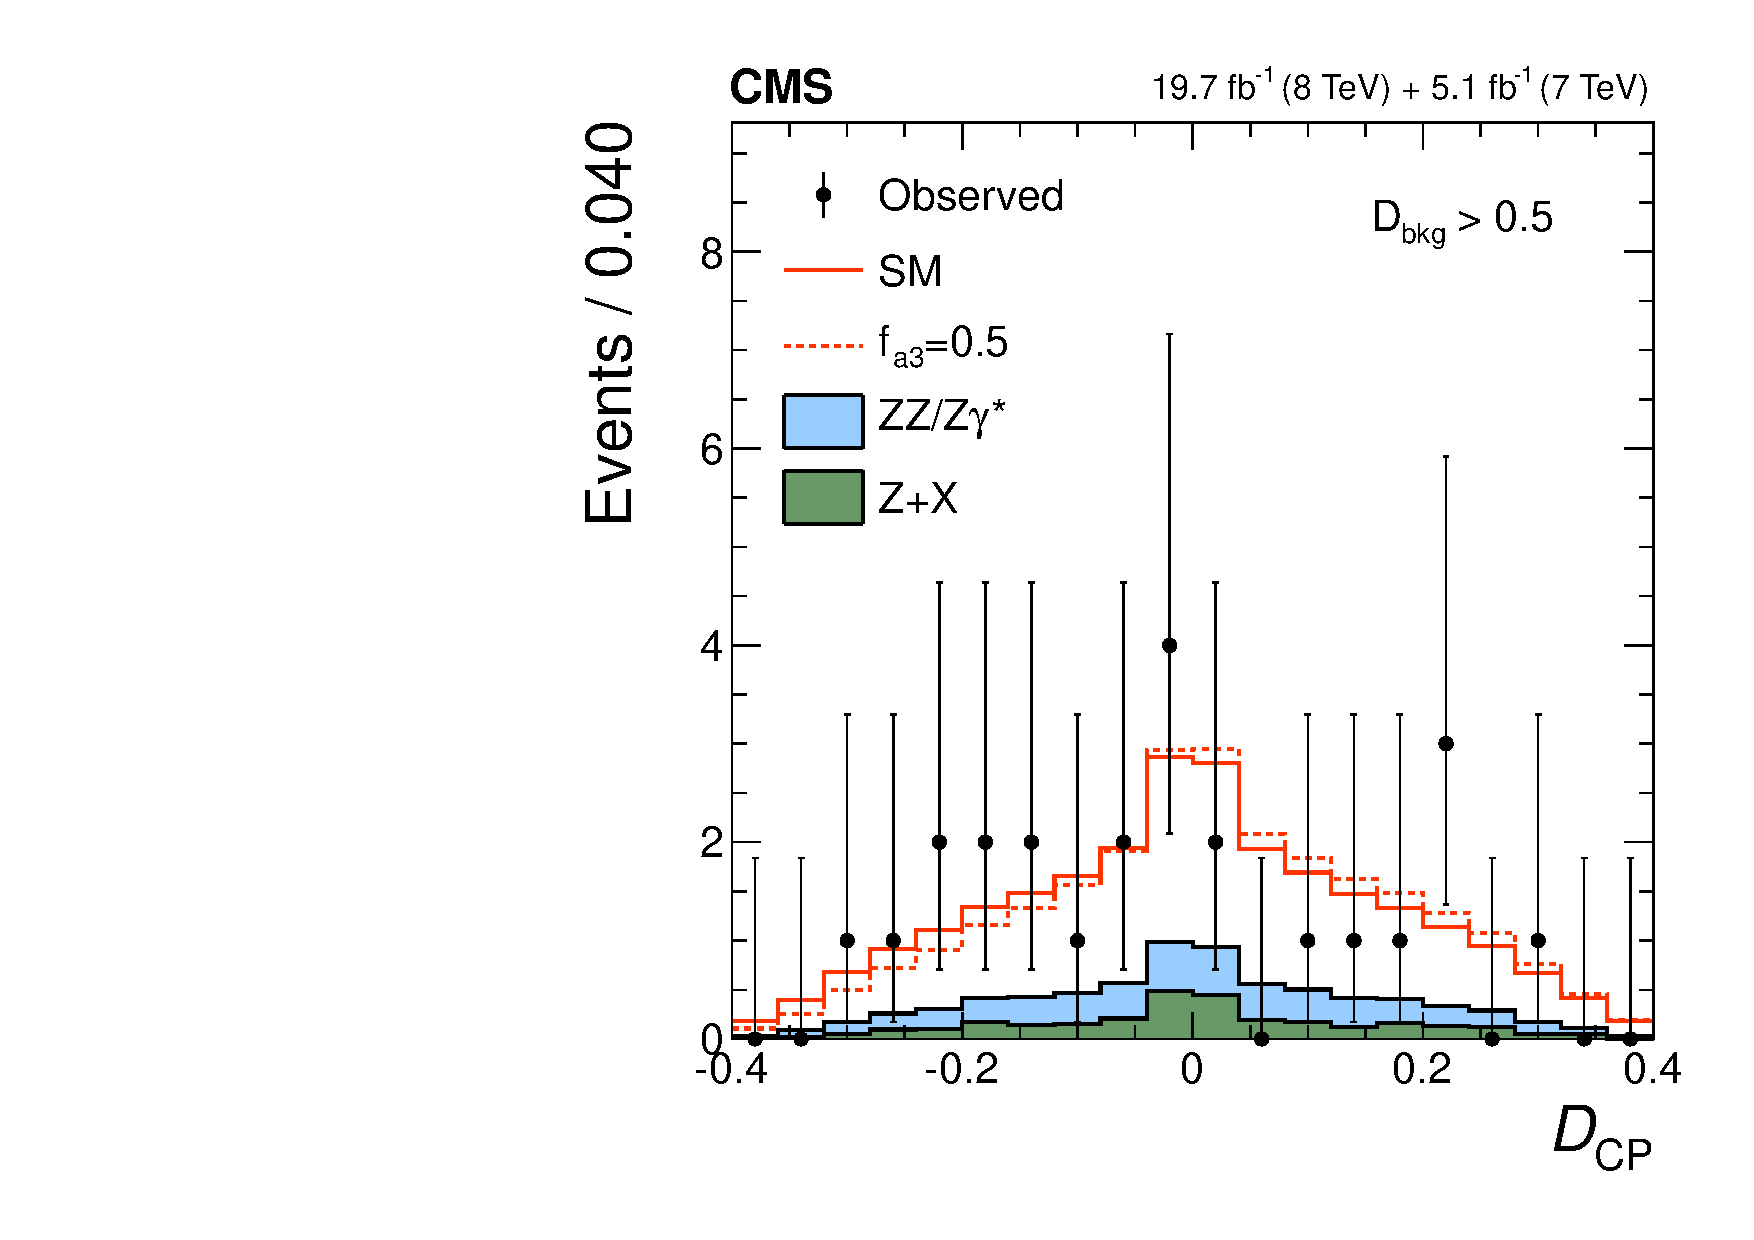
\includegraphics[width=0.32\textwidth]{Spin_Parity/cCompare_DataMC_AllTeV_D_g4int_phi0_SignalEnriched.pdf}
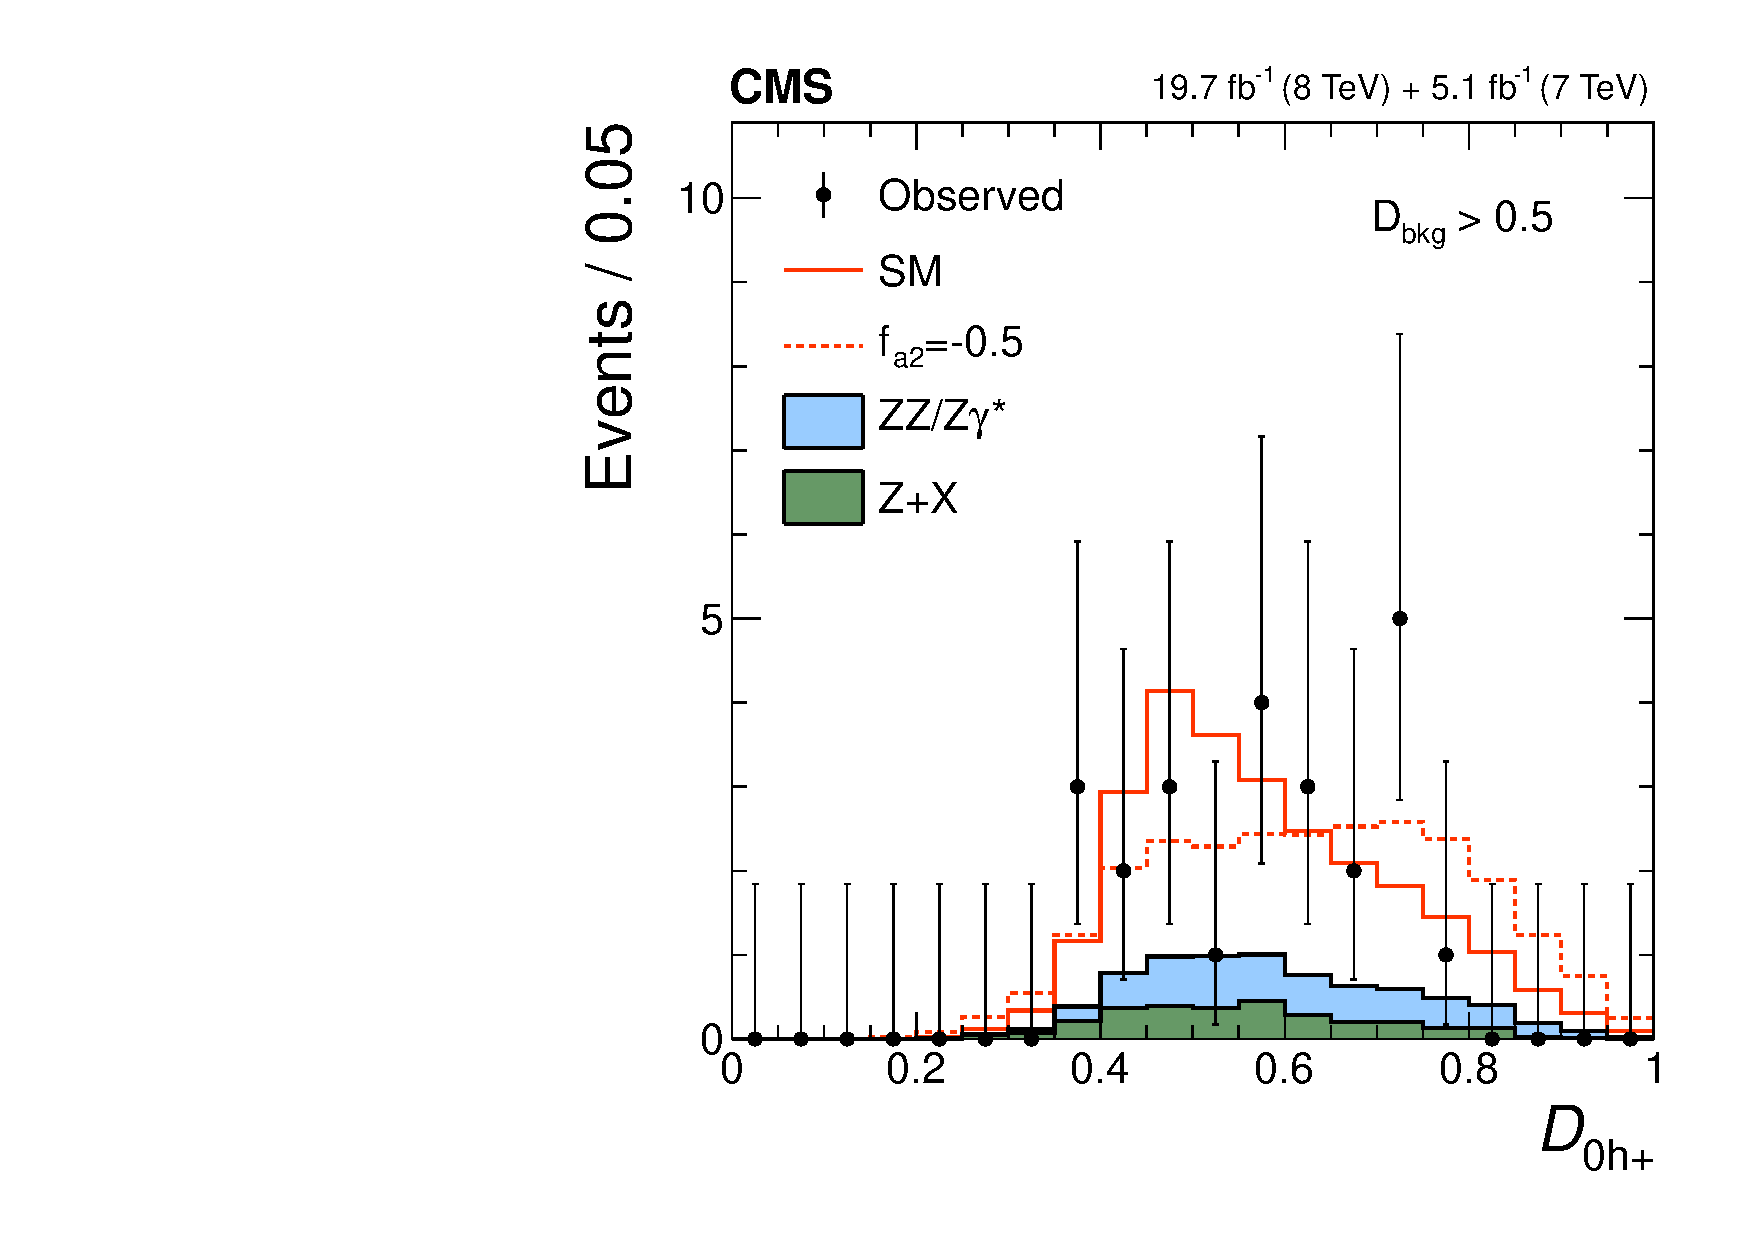
\includegraphics[width=0.32\textwidth]{Spin_Parity/cCompare_DataMC_AllTeV_D_g1_vs_g2_phi0_SignalEnriched.pdf}
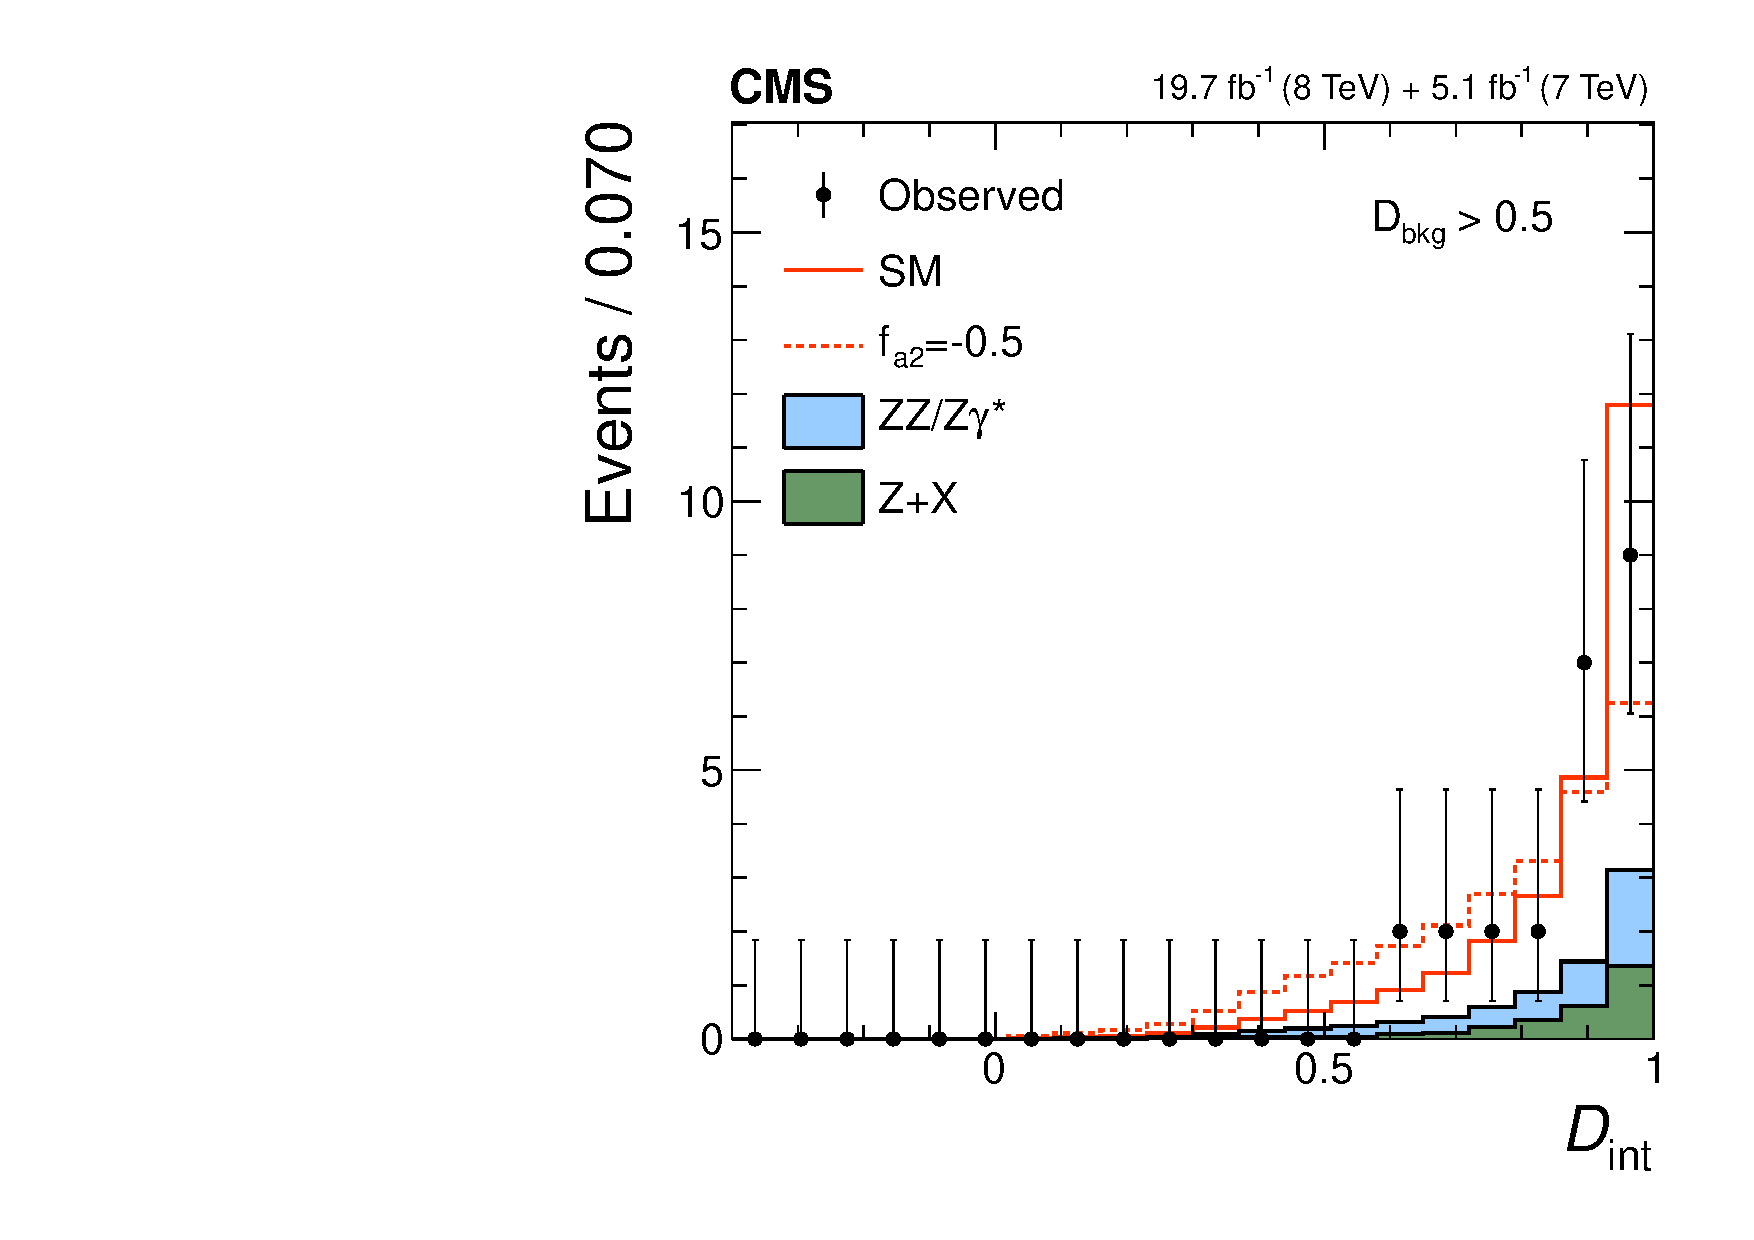
\includegraphics[width=0.32\textwidth]{Spin_Parity/cCompare_DataMC_AllTeV_D_g2int_phi0_SignalEnriched.pdf}
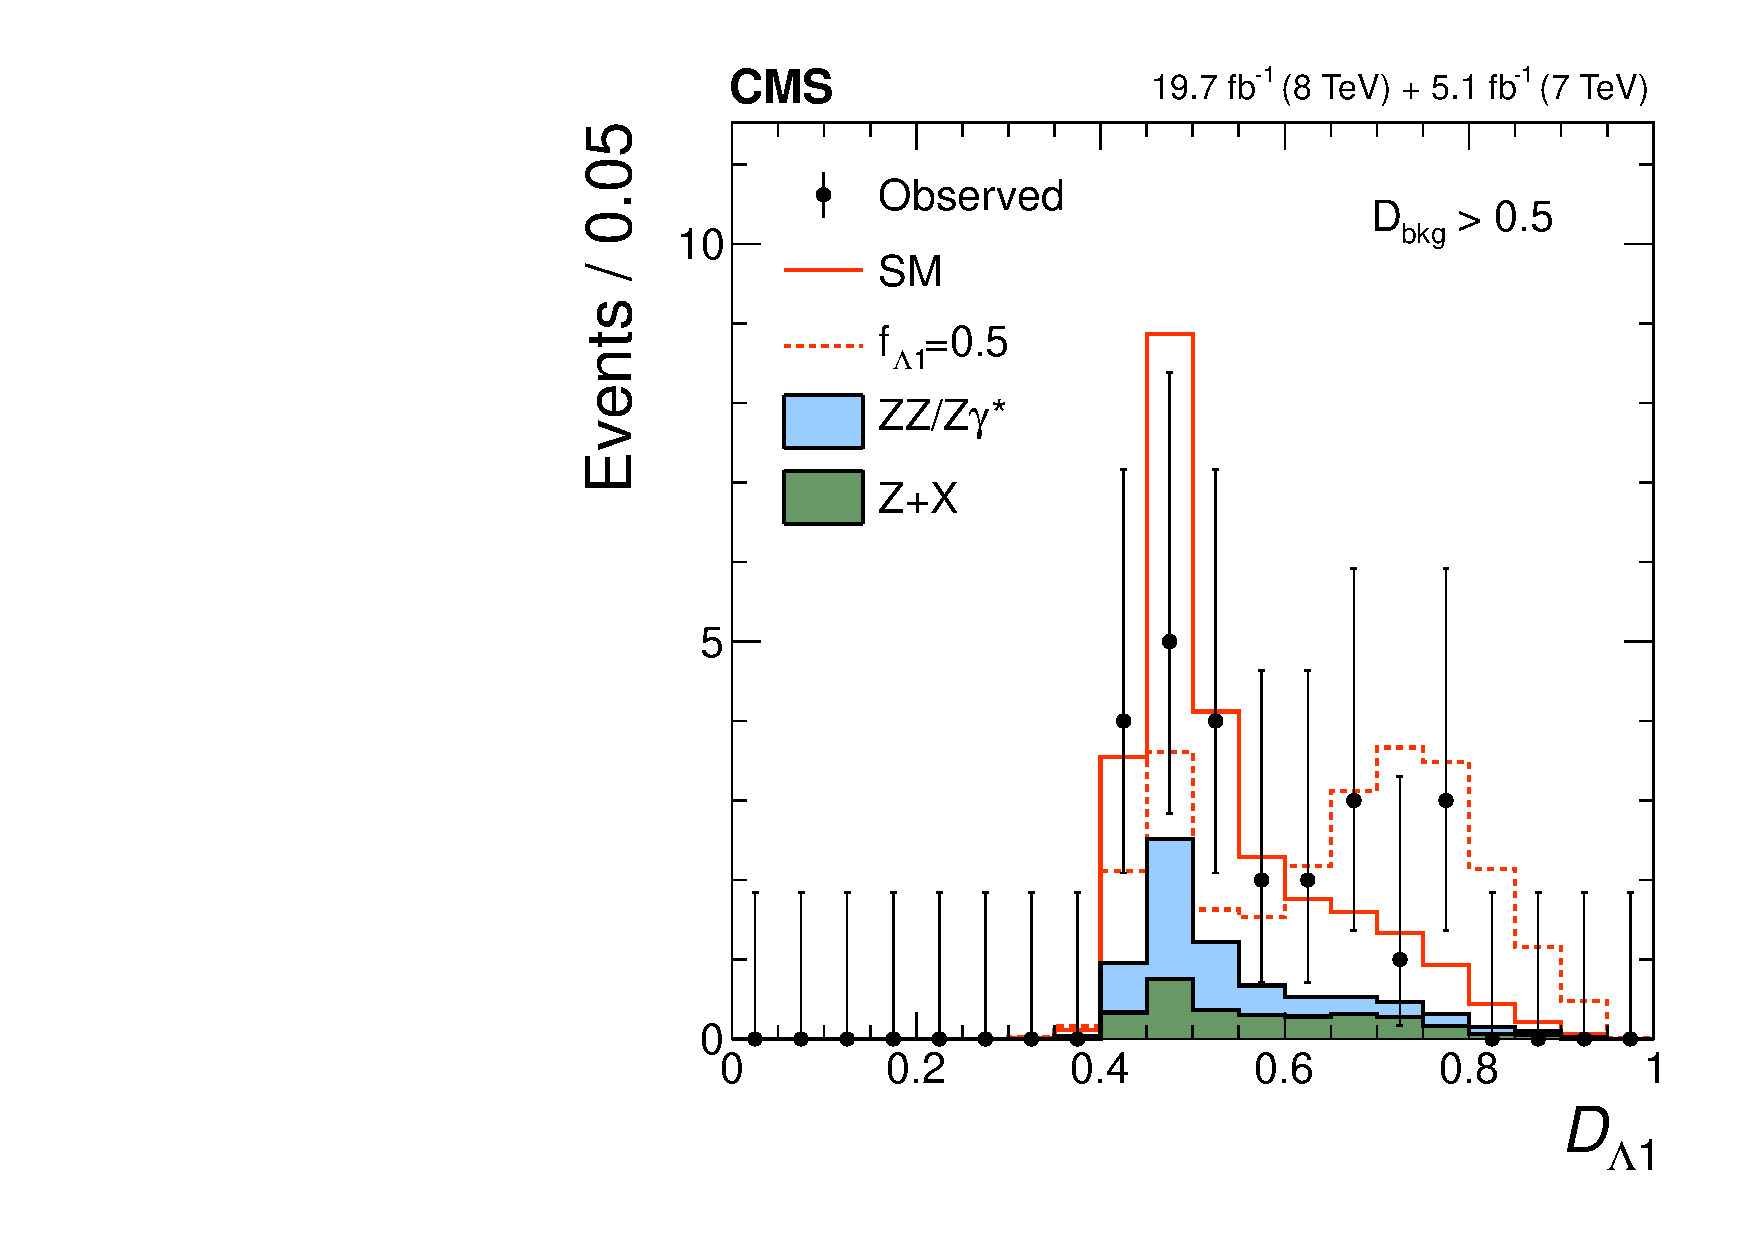
\includegraphics[width=0.32\textwidth]{Spin_Parity/cCompare_DataMC_AllTeV_D_g1Q2_phi0_SignalEnriched.pdf}
\caption[Distributions of the kinematic discriminants for
the observed data (points with error bars), the expectations for the SM background (shaded areas),
the SM Higgs boson signal (open areas under the solid histogram),
and the alternative spin-zero resonances (open areas under the dashed histograms) are shown,
as indicated in the legend.
The mass of the resonance is taken to be $\unit{125.6}{\GeV}$ and the SM cross section is used.
Top row from left to right:
$\mathcal{D}_\text{bkg}$,
$\mathcal{D}_{0-}$,
$\mathcal{D}_{C\!P}$;
bottom row from left to right:
$\mathcal{D}_{0h+}$,
$\mathcal{D}_\text{int}$,
$\mathcal{D}_{\Lambda1}$.
All distributions, with the exception of $\mathcal{D}_\text{bkg}$, are shown
with the requirement $\mathcal{D}_\text{bkg}>0.5$ to enhance signal purity.]{
Distributions of the kinematic discriminants for
the observed data (points with error bars), the expectations for the SM background (shaded areas),
the SM Higgs boson signal (open areas under the solid histogram),
and the alternative spin-zero resonances (open areas under the dashed histograms) are shown,
as indicated in the legend.
The mass of the resonance is taken to be $\unit{125.6}{\GeV}$ and the SM cross section is used.
Top row from left to right:
$\mathcal{D}_\text{bkg}$,
$\mathcal{D}_{0-}$,
$\mathcal{D}_{C\!P}$;
bottom row from left to right:
$\mathcal{D}_{0h+}$,
$\mathcal{D}_\text{int}$,
$\mathcal{D}_{\Lambda1}$.
All distributions, with the exception of $\mathcal{D}_\text{bkg}$, are shown
with the requirement $\mathcal{D}_\text{bkg}>0.5$ to enhance signal purity \cite{Khachatryan:2014kca}.
}
\label{fig:discriminants}

\end{figure}


\section{Spin/Parity Results}
\label{sec:SpinParity_Results}

Before giving a detailed description of the likelihoods that are created for this analysis and discussion of thef results, we will give a brief description of the systematic uncertainties used in this analysis.

The systematic uncertainties in the $H \to VV \to 4\ell$ channel are generally the same as the ones investigated in~\cite{Chatrchyan:2013mxa}. Among the yield uncertainties, experimental systematic uncertainties are evaluated from data for the lepton trigger efficiency and combined object reconstruction, identification, and isolation efficiencies.
The theoretical uncertainties on the $ZZ$ background are described in \cite{Chatrchyan:2013mxa}, but the calculations have been updated using the recommendations in \cite{Heinemeyer:2013tqa}
and the treatment of the $gg \to ZZ/Z\gamma^*$ process follows \cite{Khachatryan:2014iha}.
The $Z+\text{jets}$ uncertainties include the effects on both the expected yields and on the shape.
The yield uncertainties are estimated to be 20\%, 25\%, and 40\% for the $4e$, $2e2\mu$, and $4\mu$
decay channels, respectively. The shape uncertainty is taken into account by considering the difference
between the $Z+\text{jets}$ and $q\bar{q} \to ZZ$ distributions for a particular final state, which was found to cover
any potential biases in $Z+\text{jets}$ parameterization.
To account for the lepton momentum scale and resolution uncertainty in
the $m_{4\ell}$ distribution, the alternative signal shapes are taken from the variations of both of these
contributions, following~\cite{Chatrchyan:2013mxa}.

\subsection{Likelihood fits} 
\label{sec:MLfit}

The goal of the analysis is to determine if a set of anomalous coupling parameters $\vec{\zeta}$,
defined both for the production and decay of a resonance with either spin zero, one, or two
is consistent, for a given set of observables $\vec{x}$, with the data.
The coupling parameters $\vec{\zeta}$ are discussed in detail in section~\ref{sec:General_Spin_Parity}.
They are summarized in equations \eqref{eq:formfact-fullampl-spin0}, \eqref{eq:fa_definitions}
and table~\ref{tab:xsec_ratio} for spin-zero, in equations \eqref{eq:ampl-spin1} and \eqref{eq:fa_definitions_spin1} for spin-one, and in equation \eqref{eq:ampl-spin2-a} and table~\ref{tab:scenarios} for spin-two.
The observables $\vec{x}_i$ are defined for each event $i$, listed in table~\ref{tab:kdlist},
and discussed above. The extended likelihood function is defined for $N$ candidate events as
\begin{equation}
\mathcal{L} =  \exp\Big( - n_\text{sig}-\sum_k n_\text{bkg}^k  \Big)
\prod_i^{N} \Big( n_\text{sig} \times\mathcal{P}_\text{sig}(\vec{x}_{i};~\vec{\zeta})
+\sum_k n_\text{bkg}^{k} \times\mathcal{P}_\text{bkg}^k(\vec{x}_{i})
\Big),
\label{eq:likelihood}
\end{equation}

where $n_\text{sig}$ is the number of signal events and $n_\text{bkg}^k$ is the number of background events of type $k$.
The probability density functions $\mathcal{P}_\text{sig}(\vec{x}_{i};\vec{\zeta})$ and $\mathcal{P}_\text{bkg}^k(\vec{x}_{i})$
are defined for the signal and background, respectively.

There are several event categories, such as $4e$, $4\mu$, and $2e2\mu$ in the
$H\to VV \to 4\ell$ analysis, or the $\unit{7}{\TeV}$ and $\unit{8}{\TeV}$ categories, and several types of background.
The total signal yield $n_\text{sig}$ is a free parameter to avoid
using the overall signal event yield as a part of the discrimination between alternative hypotheses.
However, when several channels are used in the same decay,
such as $H \to VV \to 4e$, $2e2\mu$, and $4\mu$,
the relative yields between the channels depend on the terms considered in the tensor structure
due to interference effects in the presence of identical leptons,
and this information is exploited in the analysis.

The probability density functions $\mathcal{P}_\text{sig}$ and  $\mathcal{P}_\text{bkg}^k$ are described
as histograms (templates) with two or three dimensions, see observables in table~\ref{tab:kdlist},
and with up to 50 bins in each dimension. The number of dimensions used is limited by the number
of simulated events that can be generated or the number of events in the control regions in data.
However, an optimal construction of observables allows for the retention of all the necessary information for
the measurement with up to three observables. The templates are built for signal and background from
histograms of fully simulated events, or from control regions in data. In the $H\to VV \to 4\ell$ analyses, statistical fluctuations are removed using a smoothing algorithm~\cite{rosenblatt1956, parzen1962}.

The signal probability density functions $\mathcal{P}_\text{sig}$ depend on the coupling parameters $\vec{\zeta}$.
For spin-zero, these functions can be parameterized as a linear combination of the terms originating from
the SM-like and anomalous amplitudes and their interference~\cite{Anderson:2013afp}
\begin{multline}
\mathcal{P}_\text{sig}\left(\vec{x}; \vec{\zeta}=\{f_{ai},\phi_{ai}\}\right) =  \left(1-\sum_{ai} f_{ai}\right) \, \mathcal{P}_{0^+}\left(\vec{x}\right)
 + \sum_{ai} f_{ai} \, \mathcal{P}_{ai}\left(\vec{x}\right)  \\
+ \sum_{ai} \sqrt{f_{ai}\left(1-\sum_{aj} f_{aj}\right)}\, \mathcal{P}^\text{int}_{ai,0^+}\left(\vec{x}; \phi_{ai}\right) \\
+ \sum_{ai<aj} \sqrt{f_{ai}f_{aj}} \, \mathcal{P}^\text{int}_{ai,aj}\left(\vec{x}; \phi_{ai}-\phi_{aj}\right),
\label{eq:fractions-general}
\end{multline}

where $\mathcal{P}_{ai}$ is the probability of a pure $a_i$ term and $\mathcal{P}^\text{int}_{ai, aj}$ describes
the interference between the two terms, each parameterized as a template.
Each term in equation \eqref{eq:fractions-general} is extracted from the dedicated simulation
and includes proper normalization.

The likelihood in equation \eqref{eq:likelihood} can be used in two different ways.
In both approaches, the likelihood is maximized with respect to the nuisance parameters which include the signal yield
and constrained parameters describing the systematic uncertainties discussed above.

In one approach the likelihood is maximized to estimate the values of anomalous couplings, and the confidence intervals are determined from profile likelihood scans of the respective parameters. This is used for the measurement of anomalous
couplings under the spin-zero hypothesis. The allowed 68\% and 95\% C.L. intervals are defined using the profile likelihood function, $-2\,\Delta \ln{\mathcal L} = 1.00$ and 3.84, for which exact coverage is expected in the asymptotic limit~\cite{Wilks:1938dza}.

The other approach is used to distinguish an alternative spin-one or spin-two signal hypothesis from the SM Higgs boson.
In this case, the test statistic $q=-2{\ln(\mathcal{L}_{J^P}/\mathcal{L}_{0^+})}$ is defined using the ratio
of signal plus background likelihoods for two signal hypotheses. To quantify the consistency of the observed test statistic
$q_\text{obs}$ with respect to the SM Higgs boson hypothesis ($0^+$), the probability $p = P( q \leq q_\text{obs} \, | \, 0^+ +\text{bkg} )$ is assessed and converted into a number of standard deviations via the Gaussian one-sided tail integral.
The consistency of the observed data with the alternative signal hypothesis ($J^P$) is assessed from
$P( q \geq q_\text{obs} \, | \, J^P + \text{bkg} )$. The $CL_{s}$ criterion~\cite{Read:2002hq,Junk:1999kv}, defined
as $CL_{s} = { P( q \geq q_\text{obs} \, | \, J^P + \text{bkg} ) }$ / ${ P( q \geq q_\text{obs} \, | \, 0^+ + \text{bkg} ) } < \alpha,$
is used for the final inference of whether a particular alternative signal hypothesis is excluded or not at a given confidence level $(1 -\alpha)$.

\subsection{Exotic-spin study with the $H \to ZZ \to 4\ell$ channel}
\label{sec:ResultsExotic}

The study of the exotic-spin $J^P$ hypotheses of the observed boson with mass of $\unit{125.6}{\GeV}$ using the $X \to ZZ$ decay channel is summarized in this section. Mixed spin-one state hypotheses, as well as the spin-two models listed in table~\ref{tab:kdlist} are examined.

In the case of the spin-one studies, the hypothesis testing is performed for a discrete set of values of the parameter $f_{b2}$. The input observables are $\left(\mathcal{D}_\text{bkg}, \mathcal{D}_{1-}, \mathcal{D}_{1+}\right)$. It has been demonstrated in the context of this study that the distributions of these observables are not sensitive to the phase between the $b_1$ and $b_2$ coupling parameters in equation \eqref{eq:ampl-spin1} and therefore the results of the $f_{b2}$ scan are valid for any value of the phase term in the interference. The spin-one hypothesis is tested for
two scenarios, $q\bar{q}$ production and using only decay information. The latter requires the input observables $\left(\mathcal{D}_\text{bkg}^\text{dec},\mathcal{D}_{1-}^\text{dec},\mathcal{D}_{1+}^\text{dec}\right)$.

The expected and observed separations of spin-one models from the test statistic distributions
are summarized in table~\ref{tab:jpmodels_1} and in figure \ref{fig:jp_summary_1}.
The expected separation between the alternative signal hypotheses is
quoted for two cases. In the first case, the expected SM Higgs boson
signal strength and the alternative signal cross section are
the ones obtained in the fit to the data.
The second case assumes the nominal SM Higgs boson signal strength
(defined as $\mu=1$), while the cross section for the alternative signal hypothesis is
taken to be the same as for the SM Higgs boson (the $2e2\mu$
channel at $\unit{8}{\TeV}$ is taken as a reference). Since the observed signal strength
is very close to unity, the two results for the expected separations are also similar.

All spin-one tests are consistent with the expectation for the SM Higgs boson.
While the decay-only analysis uses less information and is expected to provide weaker constraints,
the fluctuations in the observed data lead to stronger constraints for spin-one models. Any arbitrary spin-one model for the resonance observed in the $X \to ZZ\to 4\ell$ decay mode with any
mixture of parity-even and parity-odd interactions and any production mechanism is excluded at a C.L. of
99.97\% or higher.

\begin{table}
  \centering
\caption[List of spin-one models tested in the $X \to ZZ$ analysis.
The expected separation is quoted for two scenarios, for the signal production cross section
obtained from the fit to data for each hypothesis and using the SM expectation ($\mu=1$).
The observed separation shows the consistency of the observation with the SM Higgs boson model
or the alternative $J^{P}$ model, from which the $CL_{s}$ value is derived.]{
List of spin-one models tested in the $X \to ZZ$ analysis.
The expected separation is quoted for two scenarios, for the signal production cross section
obtained from the fit to data for each hypothesis and using the SM expectation ($\mu=1$).
The observed separation shows the consistency of the observation with the SM Higgs boson model
or the alternative $J^{P}$ model, from which the $CL_{s}$ value is derived \cite{Khachatryan:2014kca}.
\label{tab:jpmodels_1}
}
\begin{tabular}{lccccc}
$f_{b2} (J^P)$                 & $J^P$        &        Expected  &                       &                    &               \\
Model                          & Prod. &        ($\mu$=1) &  Obs. $0^+$  & Obs. $J^P$ & $CL_{s}$ \\
    \hline
     $0.0 (1^-)$             & $q\bar{q}$    &  2.9$\sigma$ (2.8$\sigma$)   & $-$1.4$\sigma$ & $+$5.0$\sigma$ & $<$0.001\%  \\
    0.2      & $q\bar{q}$    &  2.6$\sigma$ (2.6$\sigma$)   & $-$1.4$\sigma$ & $+$4.6$\sigma$ & 0.002\%  \\
    0.4      & $q\bar{q}$    &  2.5$\sigma$ (2.4$\sigma$)   & $-$1.3$\sigma$ & $+$4.4$\sigma$ & 0.005\% \\
    0.6      & $q\bar{q}$    &  2.4$\sigma$ (2.4$\sigma$)   & $-$1.2$\sigma$ & $+$4.1$\sigma$ &  0.015\% \\
    0.8      & $q\bar{q}$    &  2.4$\sigma$ (2.4$\sigma$)   & $-$1.0$\sigma$ & $+$4.0$\sigma$ &  0.021\%  \\
    $1.0 (1^+)$             & $q\bar{q}$    &  2.4$\sigma$ (2.4$\sigma$)   & $-$0.8$\sigma$ & $+$3.8$\sigma$ &  0.031\%  \\
   \hline
    $0.0 (1^-)$             & any               &  2.9$\sigma$ (2.7$\sigma$)   & $-$2.0$\sigma$ & $>$5.0$\sigma$ & $<$0.001\%  \\
    0.2      & any               &  2.7$\sigma$ (2.5$\sigma$)   & $-$2.2$\sigma$ & $>$5.0$\sigma$ & $<$0.001\%  \\
    0.4      & any               &  2.5$\sigma$ (2.4$\sigma$)   & $-$2.3$\sigma$ & $>$5.0$\sigma$ & $<$0.001\% \\
    0.6      & any               &  2.5$\sigma$ (2.3$\sigma$)   & $-$2.4$\sigma$ & $>$5.0$\sigma$ & $<$0.001\%  \\
    0.8      & any               &  2.4$\sigma$ (2.3$\sigma$)   & $-$2.3$\sigma$ & $>$5.0$\sigma$ & $<$0.001\%  \\
    $1.0 (1^+)$             & any               &  2.5$\sigma$ (2.3$\sigma$)   & $-$2.3$\sigma$ & $>$5.0$\sigma$ & $<$0.001\%  \\
  \end{tabular}
\end{table}

\begin{figure}
  \centering
    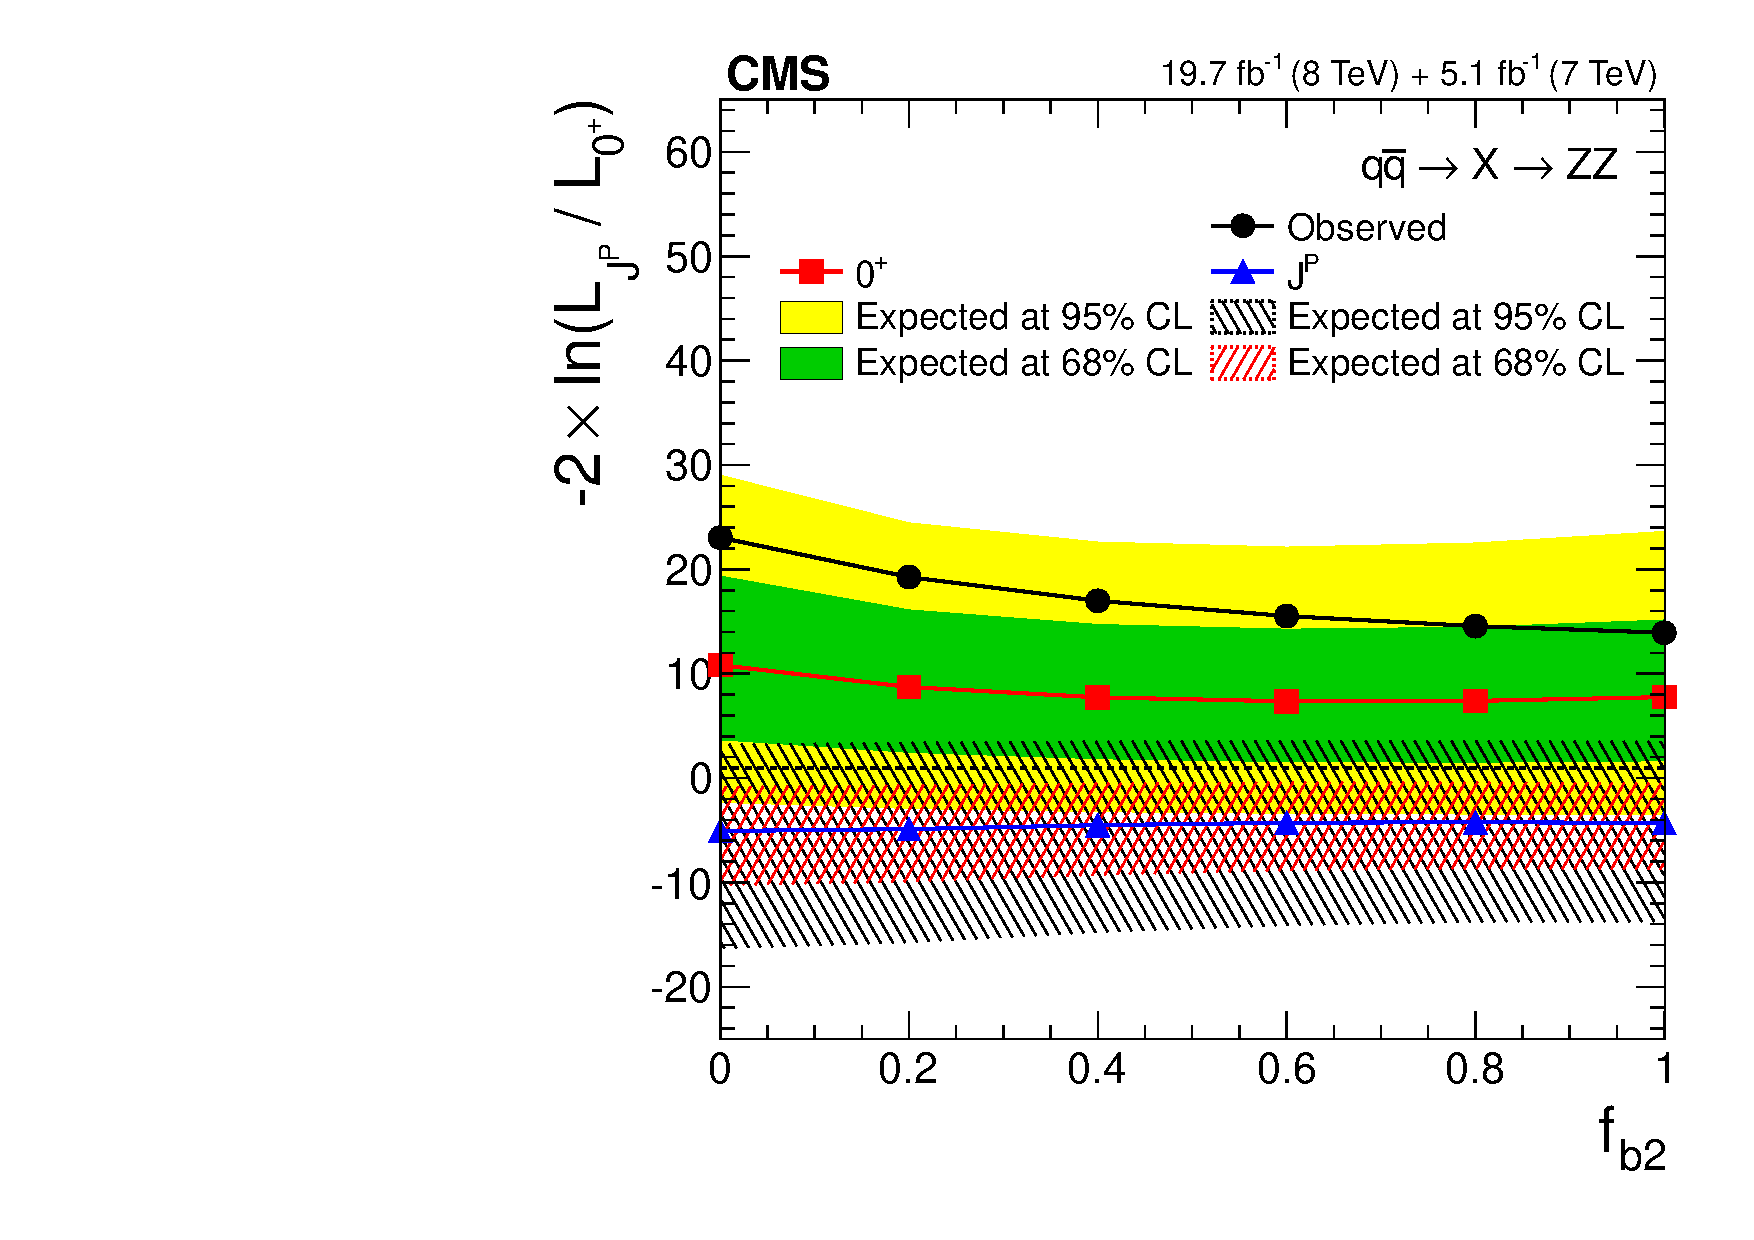
\includegraphics[width=0.45\textwidth]{Spin_Parity/summary_PD.pdf}
    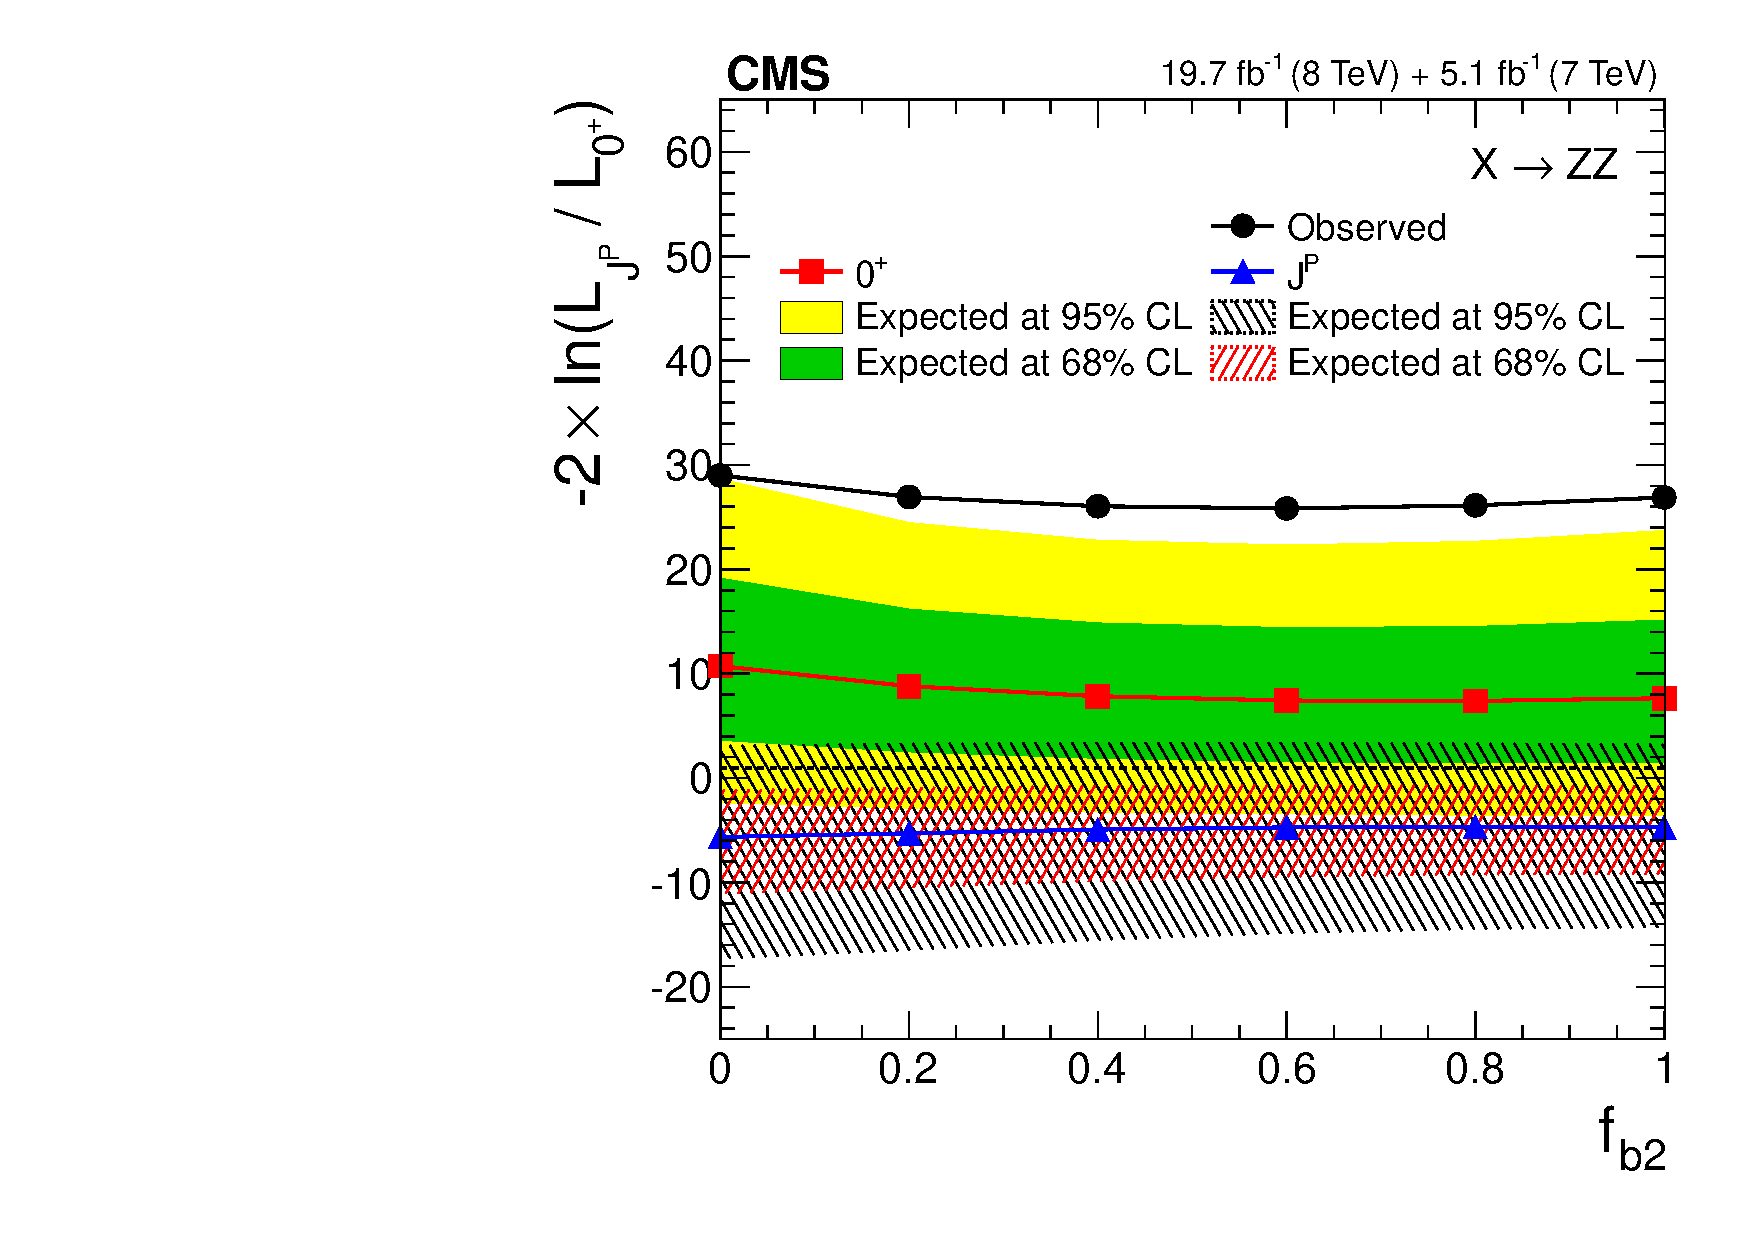
\includegraphics[width=0.45\textwidth]{Spin_Parity/summary_PI.pdf}
    \caption[Distributions of the test statistic $q=-2\ln(\mathcal{L}_{J^P}/\mathcal{L}_{0^+})$
    as a function of $f_{b2}$
      for the spin-one $J^{P}$ models tested against the SM Higgs boson hypothesis
      in the $q\bar{q} \to X \to ZZ$ (left) and decay-only $X \to ZZ$ (right) analyses.
      The median expectation for the SM Higgs boson is represented
      by the red squares with the green (68\% C.L.) and yellow (95\% C.L.) solid color regions and
       for the alternative $J^P$ hypotheses by the blue triangles
       with the red (68\% C.L.) and blue (95\% C.L.) hatched regions.
     The observed values are indicated by the black dot.]{Distributions of the test statistic $q=-2\ln(\mathcal{L}_{J^P}/\mathcal{L}_{0^+})$
    as a function of $f_{b2}$
      for the spin-one $J^{P}$ models tested against the SM Higgs boson hypothesis
      in the $q\bar{q} \to X \to ZZ$ (left) and decay-only $X \to ZZ$ (right) analyses.
      The median expectation for the SM Higgs boson is represented
      by the red squares with the green (68\% C.L.) and yellow (95\% C.L.) solid color regions and
       for the alternative $J^P$ hypotheses by the blue triangles
       with the red (68\% C.L.) and blue (95\% C.L.) hatched regions.
     The observed values are indicated by the black dots \cite{Khachatryan:2014kca}.
      \label{fig:jp_summary_1}
      }

\end{figure}


In the case of the spin-two studies, hypothesis testing is performed for ten models and three
scenarios: $gg$, $q\bar{q}$ production, and using only decay information. Two input observables
are used since interference between the different amplitude components is not considered.
These results cover all the lowest order terms in the amplitude without considering mixing of different contributions.

The data disfavor all the spin-two $X \to ZZ \to 4\ell$ hypotheses tested in favor of the SM hypothesis
$J^P=0^+$ with $1-CL_{s}$ values larger than 99\% C.L. when only decay information is used (table~\ref{tab:jpmodels}).

\begin{table}
\caption[List of spin-two models tested in the $X \to ZZ$ analysis.
The expected separation is quoted for two scenarios, for the signal production cross section
obtained from the fit to data for each hypothesis, and using the SM expectation ($\mu=1$).
The observed separation shows the consistency of the observation with the SM Higgs boson
or an alternative $J^{P}$ model, from which the $CL_{s}$ value is derived.]{
List of spin-two models tested in the $X \to ZZ$ analysis.
The expected separation is quoted for two scenarios, for the signal production cross section
obtained from the fit to data for each hypothesis, and using the SM expectation ($\mu=1$).
The observed separation shows the consistency of the observation with the SM Higgs boson
or an alternative $J^{P}$ model, from which the $CL_{s}$ value is derived.
Results from \cite{Chatrchyan:2013mxa} are explicitly noted, otherwise all results are from \cite{Khachatryan:2014kca}.
}
\centering
{\renewcommand{\arraystretch}{0.55}
\begin{tabular}{lccccccc}
$J^P$                           & $J^P$        &        Expected  &                       &                    &                \\
Model                           & Prod. &        ($\mu$=1) &  Obs. $0^+$  & Obs. $J^P$ & $CL_{s}$  \\
\hline
$2_{m}^+$~\cite{Chatrchyan:2013mxa}     & $gg$       &  1.9$\sigma$ (1.8$\sigma$)  & $-$1.1$\sigma$  & +3.0$\sigma$  &  0.90\% \\
$2^+_{h2}$ & $gg$         & 2.0$\sigma$ (2.1$\sigma$) & $-$0.3$\sigma$ & $+$2.4$\sigma$ & 2.0\%  \\
$2^+_{h3}$ & $gg$         & 3.2$\sigma$ (3.4$\sigma$) & $+$0.3$\sigma$ & $+$3.0$\sigma$ & 0.17\%  \\
$2_{h}^+$~\cite{Chatrchyan:2013mxa}      & $gg$       &  3.8$\sigma$ (4.0$\sigma$)  & +1.8$\sigma$    & +2.0$\sigma$  &  2.3\% \\
$2_{b}^+$~\cite{Chatrchyan:2013mxa}     & $gg$       &  1.6$\sigma$ (1.8$\sigma$)  & $-$1.4$\sigma$  & +3.4$\sigma$  &  0.50\% \\
$2^+_{h6}$ & $gg$         & 3.4$\sigma$ (3.7$\sigma$) & $-$0.6$\sigma$ & $+$4.9$\sigma$ & $<$0.001\% \\
$2^+_{h7}$ & $gg$         & 3.8$\sigma$ (4.5$\sigma$) & $-$0.3$\sigma$ & $+$4.5$\sigma$ & $<$0.001\%  \\
 $2^-_{h}$~\cite{Chatrchyan:2013mxa}     & $gg$       &  4.2$\sigma$ (4.5$\sigma$)  & +1.0$\sigma$    & +3.2$\sigma$  &  0.090\%  \\
$2^-_{h9}$ & $gg$          & 2.5$\sigma$ (2.6$\sigma$) & $-$1.1$\sigma$ & $+$4.0$\sigma$ & 0.029\%  \\
$2^-_{h10}$ & $gg$         & 4.2$\sigma$ (4.3$\sigma$) & $-$0.1$\sigma$ & $+$4.8$\sigma$ & $<$0.001\%  \\
\hline
$2_{m}^+$~\cite{Chatrchyan:2013mxa}     & $q\bar{q}$       &  1.7$\sigma$ (1.7$\sigma$)  & $-$1.7$\sigma$  & +3.8$\sigma$  &  0.17\% \\
$2^+_{h2}$ & $q\bar{q}$ & 2.2$\sigma$ (2.2$\sigma$) & $-$0.8$\sigma$ & $+$3.3$\sigma$ & 0.26\% \\
$2^+_{h3}$ & $q\bar{q}$ & 3.1$\sigma$ (3.0$\sigma$) & $+$0.2$\sigma$ & $+$3.0$\sigma$ & 0.21\% \\
$2^+_{h}$  & $q\bar{q}$ & 4.0$\sigma$ (3.9$\sigma$) & $+$0.2$\sigma$ & $+$3.9$\sigma$ & 0.008\%  \\
$2^+_{b}$  & $q\bar{q}$ & 1.7$\sigma$ (1.7$\sigma$) & $-$1.9$\sigma$ & $+$4.1$\sigma$ & 0.062\%  \\
$2^+_{h6}$ & $q\bar{q}$ & 3.4$\sigma$ (3.3$\sigma$) & $-$0.2$\sigma$ & $+$4.0$\sigma$ & 0.008\%  \\
$2^+_{h7}$ & $q\bar{q}$ & 4.1$\sigma$ (3.9$\sigma$) & $+$0.4$\sigma$ & $+$3.8$\sigma$ & 0.010\%  \\
$2^-_{h}$  & $q\bar{q}$  & 4.3$\sigma$ (4.4$\sigma$) & $+$0.0$\sigma$ & $+$4.6$\sigma$ & $<$0.001\% \\
$2^-_{h9}$ & $q\bar{q}$  & 2.4$\sigma$ (2.2$\sigma$) & $+$0.5$\sigma$ & $+$2.0$\sigma$ & 3.1\%  \\
$2^-_{h10}$ & $q\bar{q}$ & 4.0$\sigma$ (3.9$\sigma$) & $+$0.4$\sigma$ & $+$4.0$\sigma$ & 0.006\%  \\
\hline
$2_{m}^+$~\cite{Chatrchyan:2013mxa}      & any                   &  1.5$\sigma$ (1.5$\sigma$)  & $-$1.6$\sigma$  & +3.4$\sigma$  &  0.71\% \\
$2^+_{h2}$ & any                                 & 1.9$\sigma$ (2.0$\sigma$) & $-$0.9$\sigma$ & $+$3.0$\sigma$ & 0.74\%  \\
$2^+_{h3}$ & any                                 & 3.0$\sigma$ (3.1$\sigma$) & $+$0.0$\sigma$ & $+$3.1$\sigma$ & 0.18\%  \\
$2^+_{h}$  & any                                 & 3.8$\sigma$ (4.0$\sigma$) & $+$0.3$\sigma$ & $+$3.6$\sigma$ & 0.025\%  \\
$2^+_{b}$  & any                                 & 1.7$\sigma$ (1.7$\sigma$) & $-$1.6$\sigma$ & $+$3.6$\sigma$ & 0.29\%  \\
$2^+_{h6}$ & any                                 & 3.3$\sigma$ (3.4$\sigma$) & $-$0.3$\sigma$ & $+$4.2$\sigma$ & 0.003\%  \\
$2^+_{h7}$ & any                                 & 4.0$\sigma$ (4.2$\sigma$) & $+$0.6$\sigma$ & $+$3.5$\sigma$ & 0.032\%  \\
$2^-_{h}$  & any                                  & 4.2$\sigma$ (4.6$\sigma$) & $-$0.2$\sigma$ & $+$4.8$\sigma$ & $<$0.001\%  \\
$2^-_{h9}$ & any                                  & 2.2$\sigma$ (2.1$\sigma$) & $-$0.6$\sigma$ & $+$2.9$\sigma$ & 0.57\%  \\
$2^-_{h10}$ & any                                 & 3.9$\sigma$ (4.0$\sigma$) & $+$0.1$\sigma$ & $+$4.3$\sigma$ & 0.002\%  \\
\end{tabular}
}
\label{tab:jpmodels}
\end{table}

\begin{figure}
  \centering
    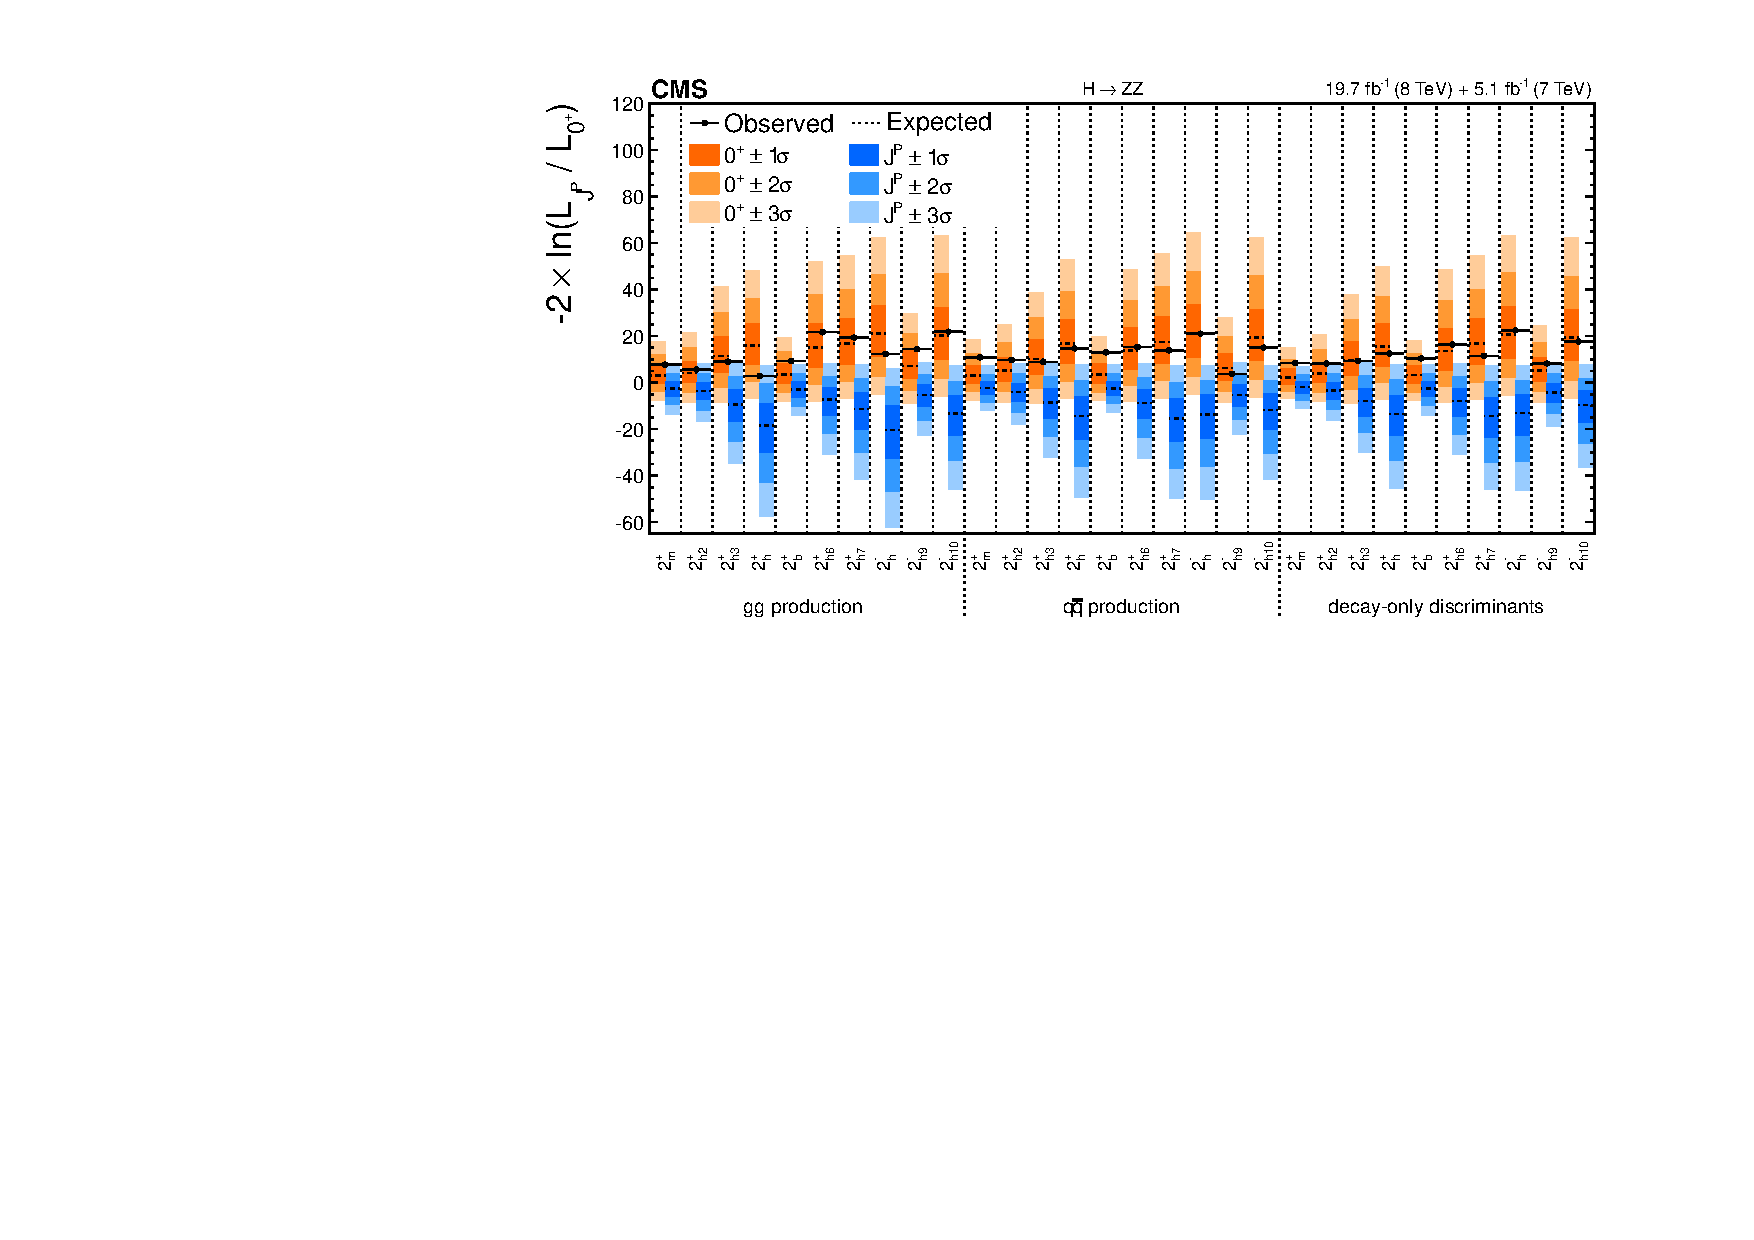
\includegraphics[width=\textwidth]{Spin_Parity/JP_SummaryPlot.pdf}
    \caption[Distributions of the test statistic $q=-2\ln(\mathcal{L}_{J^P}/\mathcal{L}_{0^+})$
       for the spin-two $J^{P}$ models tested against the SM Higgs boson hypothesis
      in the $X \to ZZ$ analyses.
      The expected median and the 68.3\%, 95.4\%, and 99.7\% C.L. regions for the SM Higgs boson (orange, the left for each model)
      and for the alternative $J^P$ hypotheses (blue, right) are shown.
     The observed $q$ values are indicated by the black dots.]{
        Distributions of the test statistic $q=-2\ln(\mathcal{L}_{J^P}/\mathcal{L}_{0^+})$
       for the spin-two $J^{P}$ models tested against the SM Higgs boson hypothesis
      in the $X \to ZZ$ analyses.
      The expected median and the 68.3\%, 95.4\%, and 99.7\% C.L. regions for the SM Higgs boson (orange, the left for each model)
      and for the alternative $J^P$ hypotheses (blue, right) are shown.
     The observed $q$ values are indicated by the black dots \cite{Khachatryan:2014kca}.
      \label{fig:jp_summary}
      }
\end{figure}

\subsection{Study of spin-zero $HVV$ couplings} \label{sec:ResultsSpinZero}
Given the exclusion of the exotic spin-one and spin-two scenarios presented in section~\ref{sec:ResultsExotic},
detailed studies of $HVV$ interactions under the assumption that the new boson is a spin-zero
resonance are performed. 

First, constraints are applied on the presence of only one anomalous term in the $HVV$
amplitude where the couplings are considered to be real. A summary of such results is presented
in table~\ref{tab:summary_spin0} and figure~\ref{fig:spin0_summary}.
The details of these and other measurements are presented in the following subsections, with further
measurements considering simultaneously up to four fractions and phase parameters in several cases.

\begin{table}
\centering
\caption[Summary of allowed 68\%~C.L. (central values with uncertainties) and 95\%~C.L. (ranges in square brackets)
intervals on anomalous coupling parameters in $HVV$ interactions under the assumption that all the coupling
ratios are real ($\phi_{ai}^{VV}=0$ or $\pi$).
The ranges are truncated at the physical boundaries of $f_{ai}^{VV}=1$.
The last column indicates the observed (expected) confidence level of a pure anomalous coupling
corresponding to $f_{ai}^{VV}=1$ when compared to the SM expectation $f_{ai}^{VV}=0$.]{
Summary of allowed 68\%~C.L. (central values with uncertainties) and 95\%~C.L. (ranges in square brackets)
intervals on anomalous coupling parameters in $HVV$ interactions under the assumption that all the coupling
ratios are real ($\phi_{ai}^{VV}=0$ or $\pi$).
The ranges are truncated at the physical boundaries of $f_{ai}^{VV}=1$.
The last column indicates the observed (expected) confidence level of a pure anomalous coupling
corresponding to $f_{ai}^{VV}=1$ when compared to the SM expectation $f_{ai}^{VV}=0$ \cite{Khachatryan:2014kca}.
}
\begin{tabular}{ccccccc}
 & Parameter                                   &  \multicolumn{2}{c}{Observed} &  \multicolumn{2}{c}{Expected}  & $f_{ai}^{VV}=1$  \\
\hline
& $f_{\Lambda1}\cos(\phi_{\Lambda1})$        & \multicolumn{2}{c}{$0.22^{+0.10}_{-0.16}$ $ [-0.25,0.37] $}          & \multicolumn{2}{c}{$0.00^{+0.16}_{-0.87}$ $ [-1.00,0.27]$}
& 1.1\% (16\%)                                    \\
&   & \multicolumn{2}{c}{ }          & \multicolumn{2}{c}{~~~~~~~~~$\cup [0.92,1.00] $}       &            \\
& $f_{a2}\cos(\phi_{a2})$         & \multicolumn{2}{c}{$0.00^{+0.41}_{-0.06}$ $ [-0.66, -0.57]$}     & \multicolumn{2}{c}{$0.00^{+0.38}_{-0.08}$ $ [-0.18,1.00]$}
 & 5.2\% (5.0\%)               \\
 &     & \multicolumn{2}{c}{~~~~~~~~~$ \cup [-0.15,1.00]$}     & \multicolumn{2}{c}{ }       &            \\
& $f_{a3}\cos(\phi_{a3})$         & \multicolumn{2}{c}{$0.00^{+0.14}_{-0.11}$ $ [-0.40,0.43] $} & \multicolumn{2}{c}{$0.00^{+0.33}_{-0.33}$ $ [-0.70,0.70] $}
& 0.02\% (0.41\%)         \\
& $f_{\Lambda1}^{WW}\cos(\phi_{\Lambda1}^{WW})$   & \multicolumn{2}{c}{$0.21^{+0.18}_{-1.21}$ $ [-1.00 ,1.00]$}     & \multicolumn{2}{c}{$0.00^{+0.34}_{-1.00}$ $[-1.00, 0.41]$}
& 78\% (67\%)        \\
& & \multicolumn{2}{c}{ }     & \multicolumn{2}{c}{~~~~~~~~~$\cup  [0.49,1.00]$}   &    \\
& $f_{a2}^{WW}\cos(\phi_{a2}^{WW})$         & \multicolumn{2}{c}{$-0.02^{+1.02}_{-0.16}$ $ [-1.00, -0.54]$}     & \multicolumn{2}{c}{$0.00^{+1.00}_{-0.12}$ $[-1.00, -0.58]$}
& 42\% (46\%)             \\
 &  & \multicolumn{2}{c}{~~~~~~~~~$\cup  [-0.29,1.00]$}     & \multicolumn{2}{c}{~~~~~~~~~$\cup  [-0.22,1.00]$}   &     \\
& $f_{a3}^{WW}\cos(\phi_{a3}^{WW})$         & \multicolumn{2}{c}{$-0.03^{+1.03}_{-0.97}$ $ [-1.00,1.00] $} & \multicolumn{2}{c}{$0.00^{+1.00}_{-1.00}$ $ [-1.00,1.00] $}
& 34\% (49\%)        \\
& $f_{\Lambda1}^{Z\gamma}\cos(\phi_{\Lambda1}^{Z\gamma})$        & \multicolumn{2}{c}{$-0.27^{+0.34}_{-0.49}$ $ [-1.00,1.00] $}          & \multicolumn{2}{c}{$0.00^{+0.83}_{-0.53}$ $[-1.00,1.00] $}
& 26\% (16\%)                                              \\
& $f_{a2}^{Z\gamma}\cos(\phi_{a2}^{Z\gamma})$          & \multicolumn{2}{c}{$0.00^{+0.14}_{-0.20}$ $[-0.49,0.46]$} &   \multicolumn{2}{c}{$0.00^{+0.51}_{-0.51}$ $[-0.78,0.79]$}
& $<$0.01\% (0.01\%)         \\
& $f_{a3}^{Z\gamma}\cos(\phi_{a3}^{Z\gamma})$           & \multicolumn{2}{c}{$0.02^{+0.21}_{-0.13}$ $[-0.40,0.51]$} &   \multicolumn{2}{c}{$0.00^{+0.51}_{-0.51}$ $[-0.75,0.75]$}
& $<$0.01\% ($<$0.01\%)         \\
 & $f_{a2}^{\gamma\gamma}\cos(\phi_{a2}^{\gamma\gamma})$    & \multicolumn{2}{c}{$0.12_{-0.11}^{+0.20}$ $[-0.04,+0.51]$} &   \multicolumn{2}{c}{$0.00_{-0.09}^{+0.11}$ $[-0.32,0.34]$}
& $<$0.01\% ($<$0.01\%)        \\
& $f_{a3}^{\gamma\gamma}\cos(\phi_{a3}^{\gamma\gamma})$    & \multicolumn{2}{c}{$-0.02_{-0.13}^{+0.06}$ $[-0.35,0.32]$} &   \multicolumn{2}{c}{$0.00_{-0.11}^{+0.15}$ $[-0.37,0.40]$}
& $<$0.01\% ($<$0.01\%)        \\
\end{tabular}
\label{tab:summary_spin0}
\end{table}

\begin{figure}
  \centering
    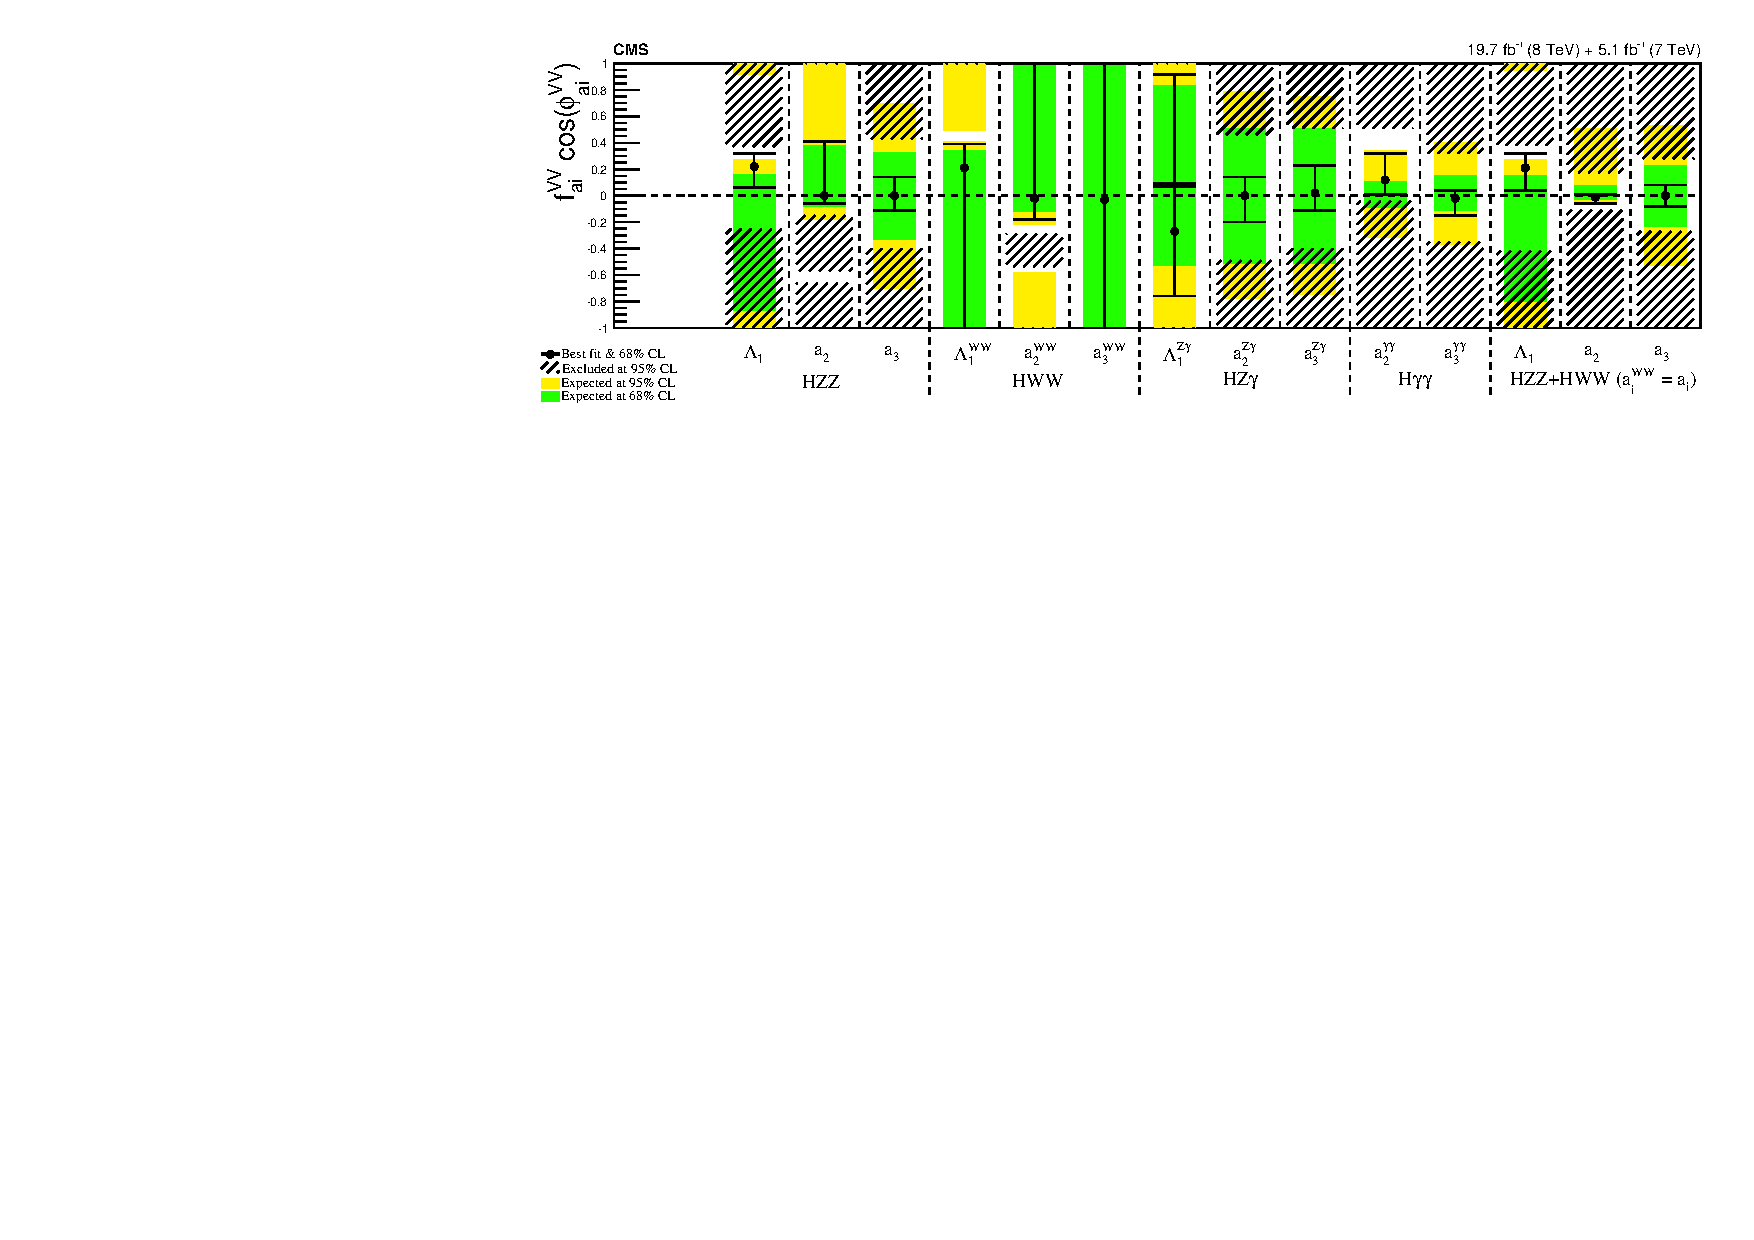
\includegraphics[width=\textwidth]{Spin_Parity/Summary_spin0.pdf}
    \caption[Summary of allowed confidence level intervals on anomalous coupling parameters in $HVV$
interactions under the assumption that all the coupling ratios are real ($\phi_{ai}^{VV}=0$ or $\pi$).
The expected 68\% and 95\% C.L. regions are shown as the green and yellow bands.
The observed constraints at 68\% and 95\% C.L. are shown as the points with errors
and the excluded hatched regions.
In the case of the $f_{\Lambda1}^{Z\gamma}$ measurement, there are two minima and two
68\%~C.L. intervals, while only one global minimum is indicated with a point.
The combination of the  $HZZ$ and $HWW$ measurements is presented,
assuming the symmetry $a_i = a_i^{WW}$.]{
Summary of allowed confidence level intervals on anomalous coupling parameters in $HVV$
interactions under the assumption that all the coupling ratios are real ($\phi_{ai}^{VV}=0$ or $\pi$).
The expected 68\% and 95\% C.L. regions are shown as the green and yellow bands.
The observed constraints at 68\% and 95\% C.L. are shown as the points with errors
and the excluded hatched regions.
In the case of the $f_{\Lambda1}^{Z\gamma}$ measurement, there are two minima and two
68\%~C.L. intervals, while only one global minimum is indicated with a point.
The combination of the  $HZZ$ and $HWW$ measurements is presented,
assuming the symmetry $a_i = a_i^{WW}$ \cite{Khachatryan:2014kca}.
      \label{fig:spin0_summary}}

\end{figure}

\subsubsection{Study of $HZZ$ couplings with the $H\to ZZ\to 4\ell$ channel} \label{sec:Resultspinzerohzz}

The study of the anomalous $HVV$ couplings starts with the test of three contributions to the $HZZ$ interaction
as shown in equation \eqref{eq:formfact-fullampl-spin0}. Only real couplings are considered in this test,
$\phi_{ai}=0$ or $\pi$, where $\phi_{ai}$ generically refers to the phase of the coupling in question,
such as $\phi_{\Lambda1}$, $\phi_{a2}$, or $\phi_{a3}$. Since the expansion of terms in equation \eqref{eq:formfact-fullampl-spin0} is considered for small anomalous contributions,
all other parameters are set to zero when the anomalous couplings of interest are considered.
These constraints of real couplings and zero contribution from other terms are relaxed in further tests
discussed below.

The results of the likelihood function scan for the three parameters, $f_{ai}\cos\phi_{ai}$, are shown in
figure \ref{fig:results_ZZ_1D} (left), where the $\cos\phi_{ai}$ term allows for a signed quantity with
$\cos\phi_{ai}=-1$ or $+1$.
The 68\% and 95\%~C.L. intervals are shown in table~\ref{tab:summary_spin0}.
These results can be interpreted for the coupling parameters
used in equation \eqref{eq:formfact-fullampl-spin0}, as shown in table~\ref{tab:Spin0zz_interpretation}.
Strong destructive interference of the SM and anomalous contributions
at $f_{\Lambda1}\cos(\phi_{\Lambda1})\sim+0.5$ or $f_{a2}\cos(\phi_{a2})\sim-0.5$
leads to very different kinematic distributions and exclusions with high confidence levels.
Additional features with multiple likelihood function maxima observed in the $f_{\Lambda1}$ likelihood scan
are due to the superposition of measurements in the $4e/4\mu$ and $2e2\mu$ channels,
which have different maxima due to the interference between the leptons.

Next, two parameters $f_{ai}$ and $\phi_{ai}$ are considered at the same time. For example, if the coupling is known
to be either positive or negative, such a scenario is considered in table~\ref{tab:Spin0_ZZ_1D_KDb}. In this
case, constraints are set on $f_{ai}$ for a given phase value. More generally, one can allow $\phi_{ai}$ to be unconstrained,
that is, to have any value between $-\pi$ and $+\pi$ with a generally complex coupling.
Such a fit is performed for $f_{\Lambda1}$ and $f_{a2}$ using the
same configuration, but with additional $\phi_{\Lambda1}$ and $\phi_{a2}$ parameters in equation \eqref{eq:fractions-general}.
The results with $\phi_{ai}$ unconstrained (any) are shown in table~\ref{tab:Spin0_ZZ_1D_KDb} as well.
The $f_{a3}$ measurement with $\phi_{a3}$ unconstrained is performed with a different technique and is presented
in \cite{Chatrchyan:2013mxa}, where the $\mathcal{D}_{C\!P}$ observable is removed from the fit and the result
becomes insensitive to the phase of the amplitude. This technique is adopted due to its simpler implementation and
equivalent performance.

The next step in generalizing the constraints is to consider two anomalous contributions at the same time, both with
and without the constraints that the couplings are real. Therefore, up to four parameters are considered at the same
time: $f_{ai}$, $\phi_{ai}$, $f_{aj}$, and $\phi_{aj}$. Constraints on one parameter, when other parameters are left unconstrained in
the full allowed parameter space, with $0\le f_{ai}\le 1$, are presented in table~\ref{tab:Spin0_ZZ_1D_KDb}.
Even though the expansion with only three anomalous contributions in equation \eqref{eq:formfact-fullampl-spin0} becomes incomplete when large values of $f_{ai}\sim 1$ are considered,
this is still a valuable test of the consistency of the data with the SM.
All of the above results, with phases fixed or unconstrained and with other anomalous couplings unconstrained
are shown in figure \ref{fig:results_ZZ_1D} (right).
Some observed $f_{ai}$ constraints appear to be tighter when compared to the one-parameter fits shown in
figure \ref{fig:results_ZZ_1D} (left). This happens because the values of other profiled parameters are away
from the SM expectation at the minimum of $-2\ln\mathcal{L}$, though still consistent with the SM.
The expected constraints are always weaker with additional free parameters.

\begin{figure}
\centering
       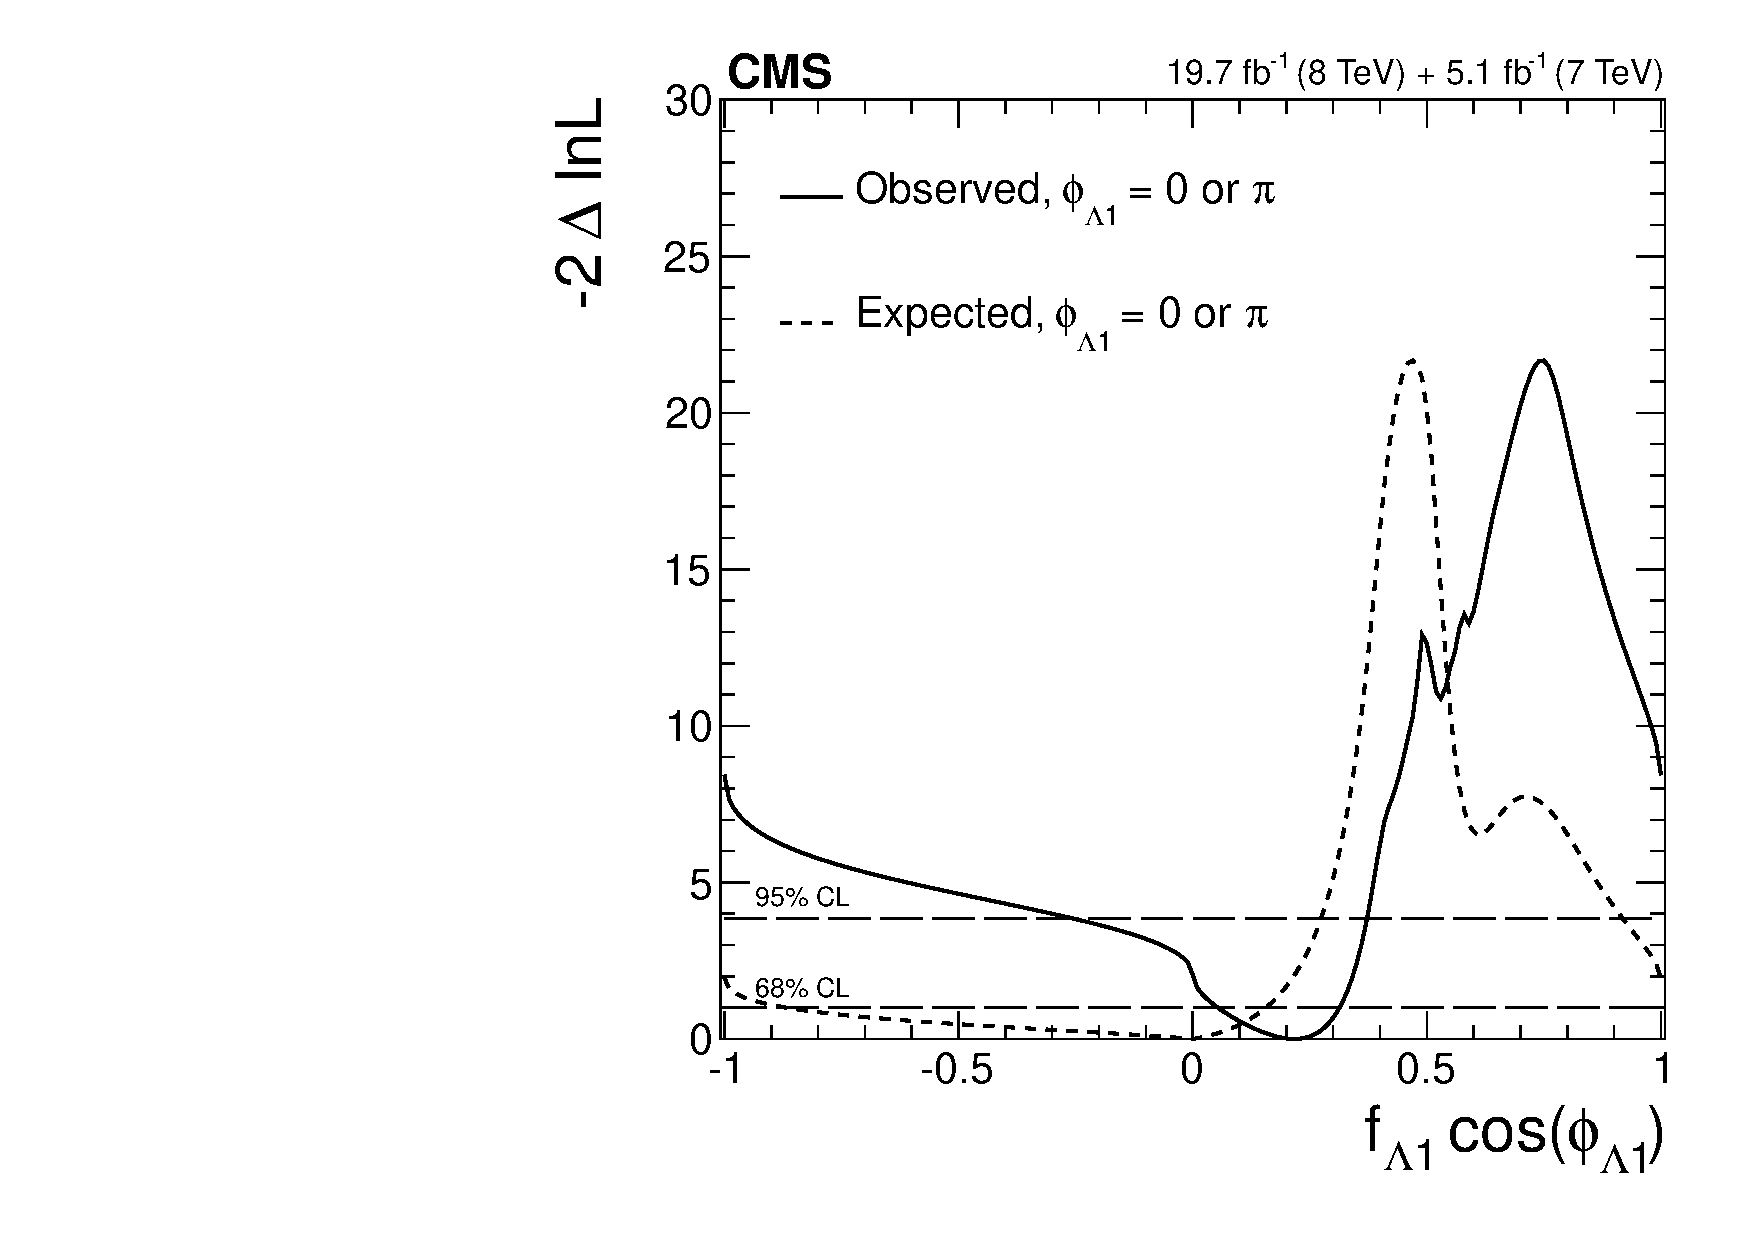
\includegraphics[width=0.38\textwidth]{Spin_Parity/fL1_Real.pdf}
       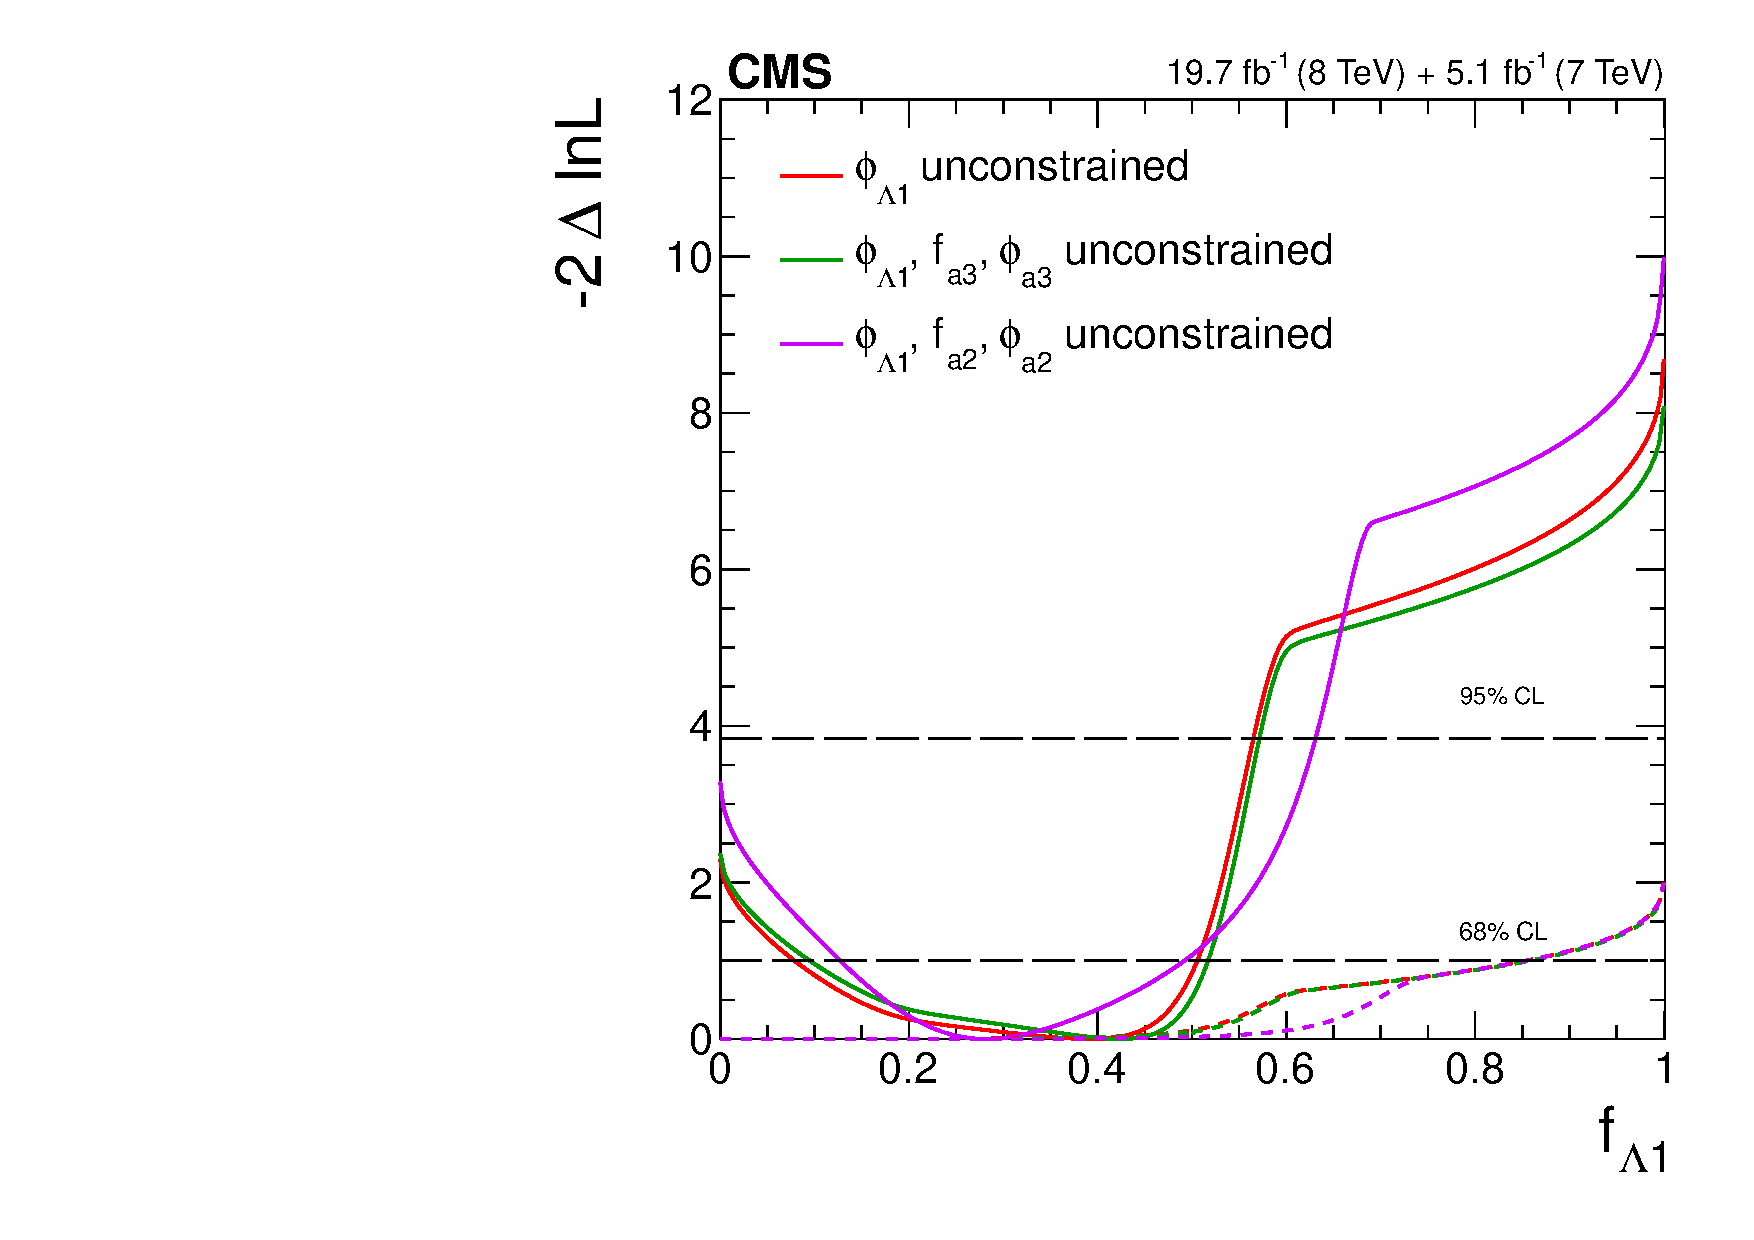
\includegraphics[width=0.38\textwidth]{Spin_Parity/fL1_Profile.pdf} \\
       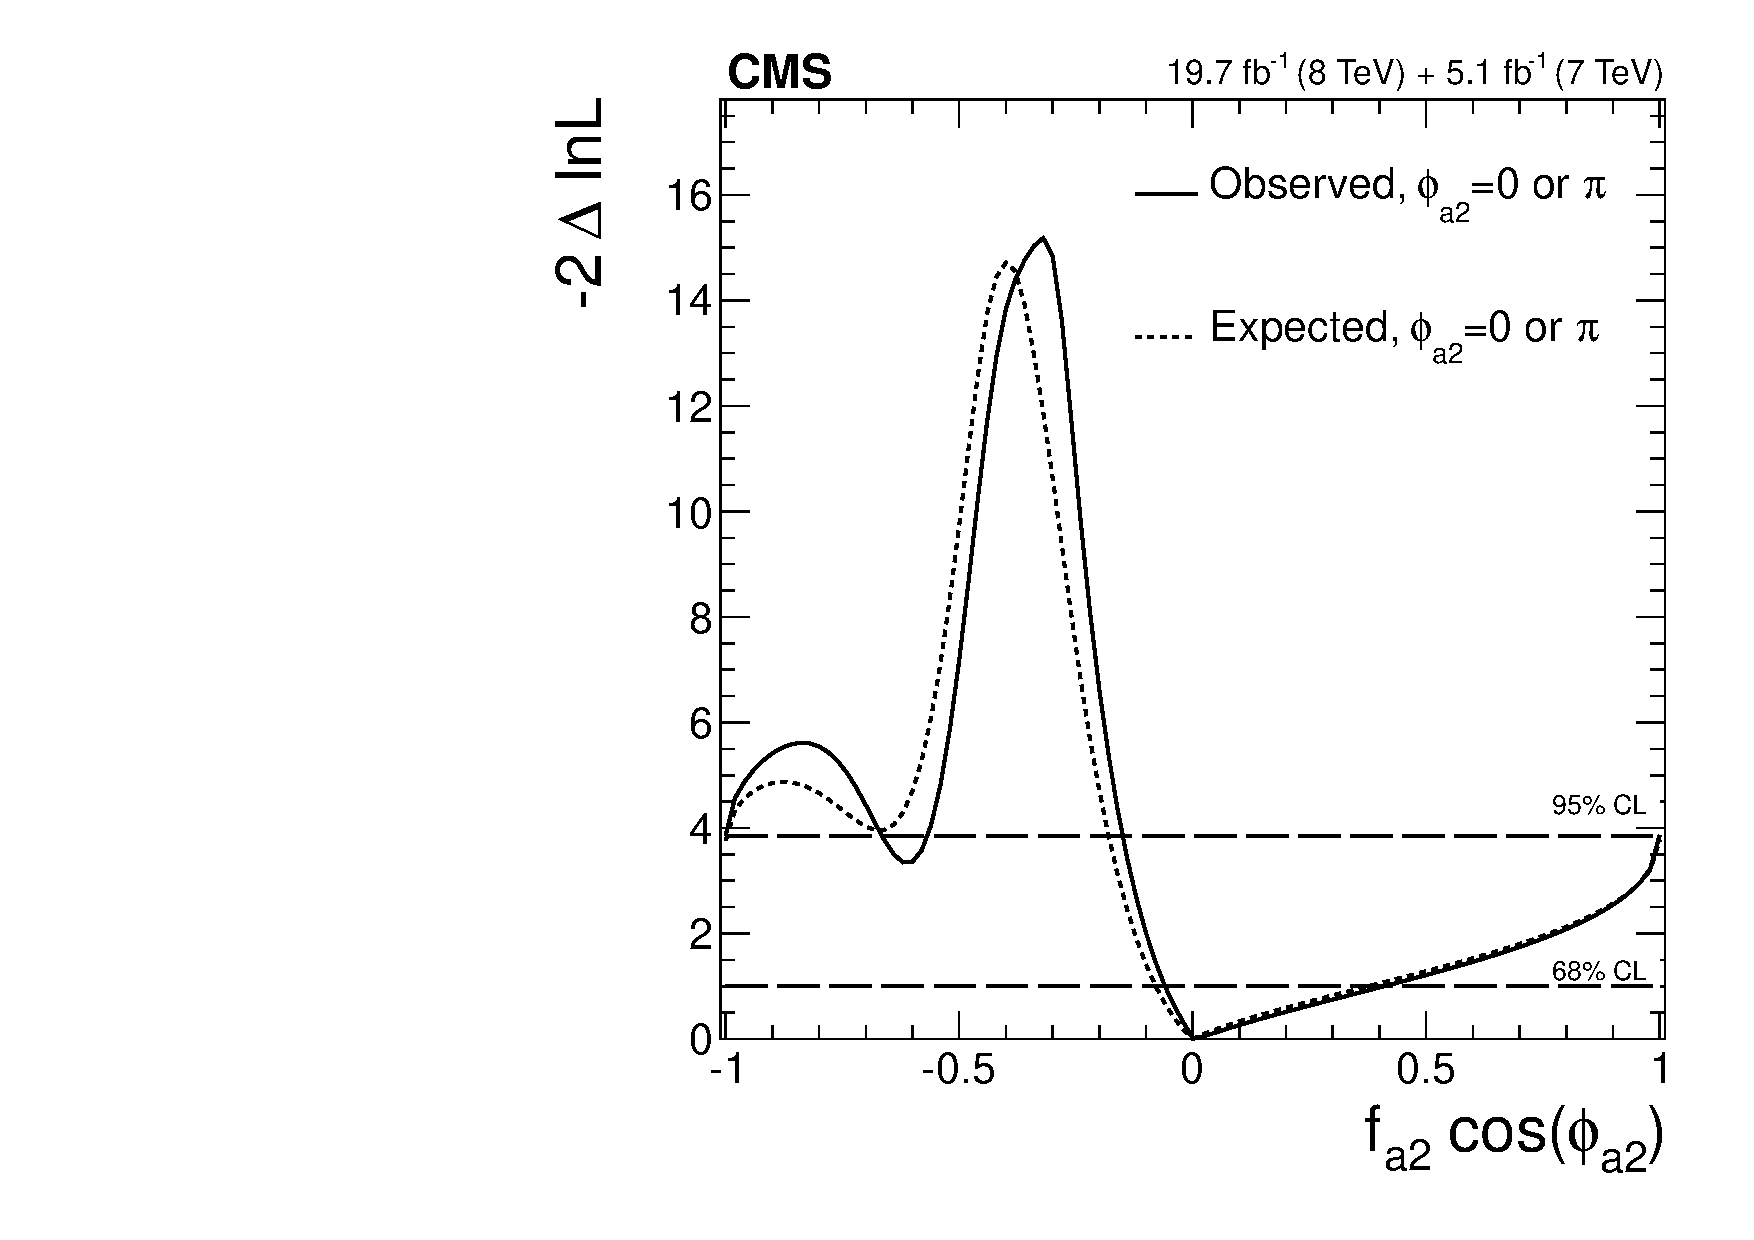
\includegraphics[width=0.38\textwidth]{Spin_Parity/fa2_Real.pdf}
       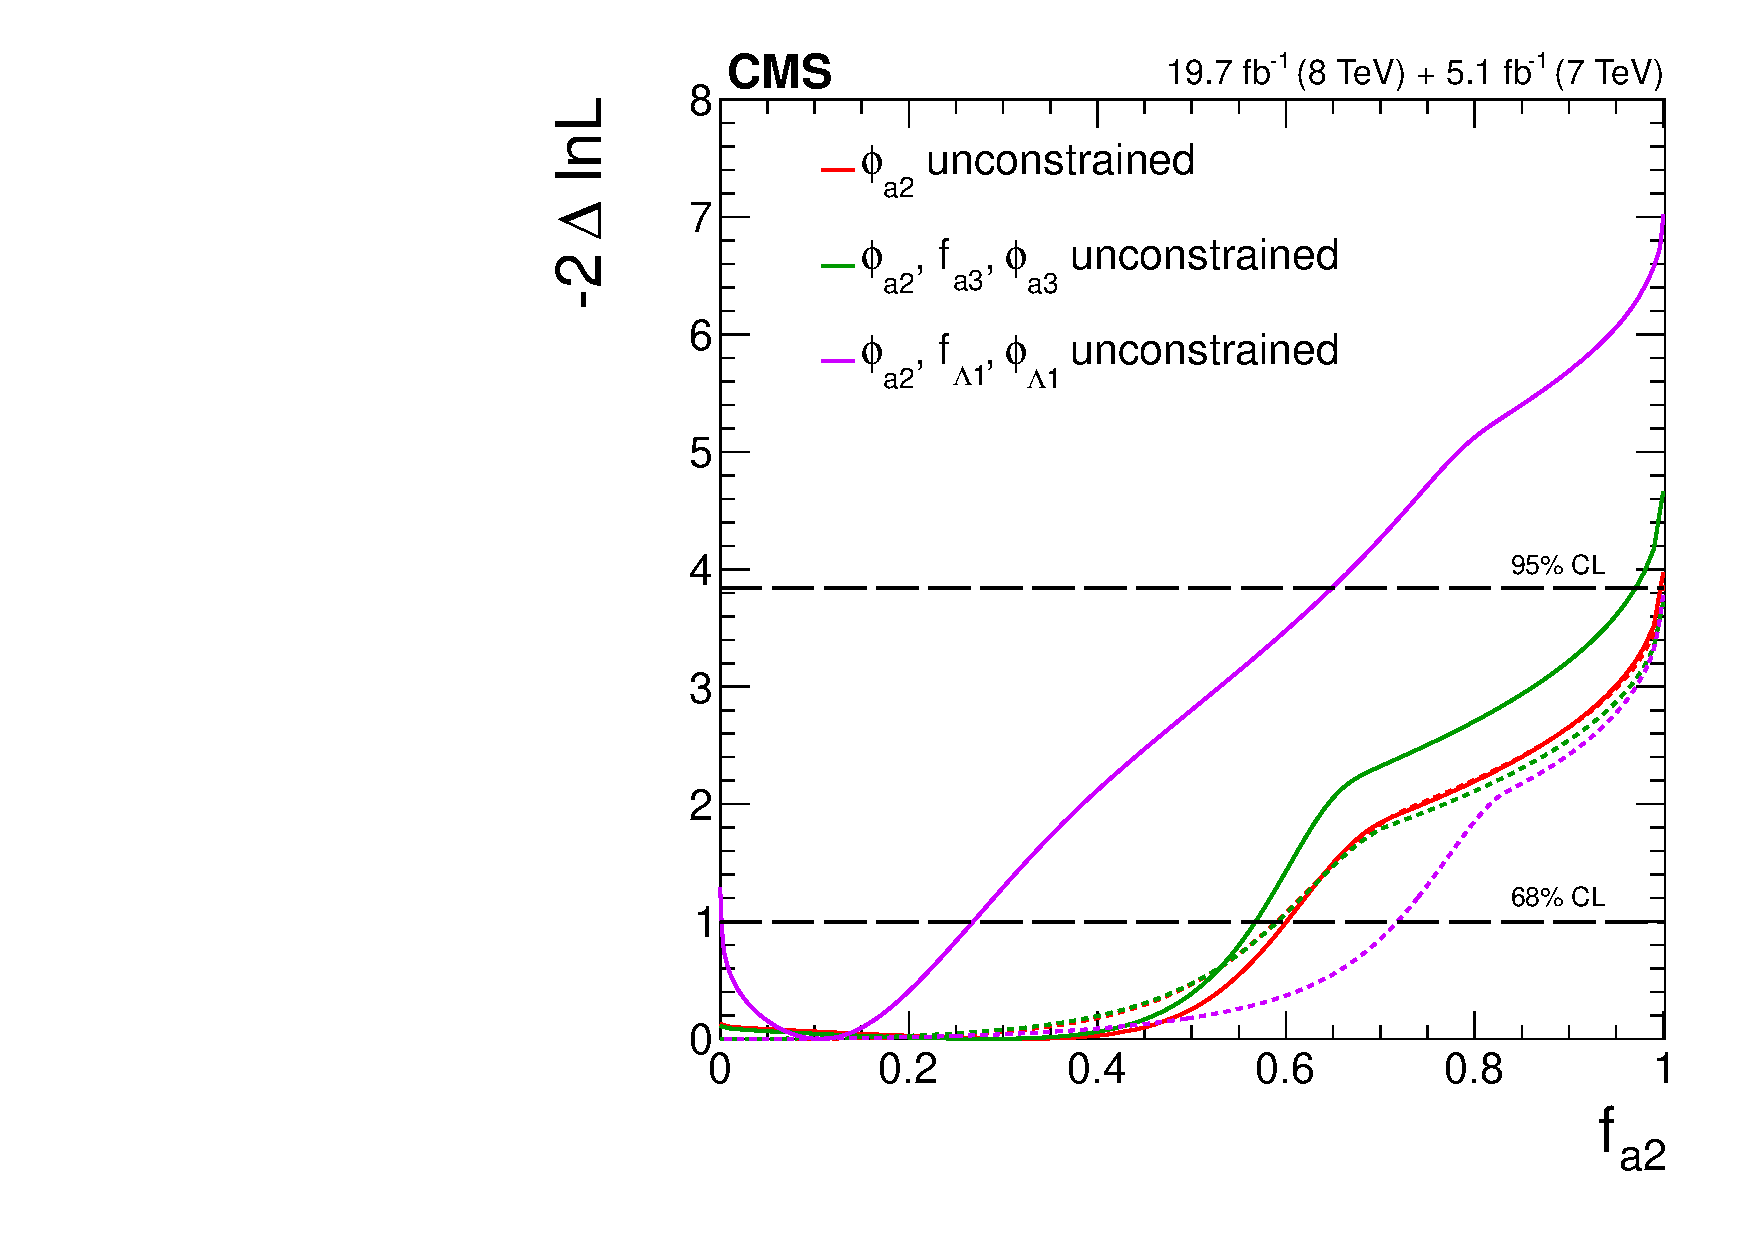
\includegraphics[width=0.38\textwidth]{Spin_Parity/fa2_Profile.pdf} \\
       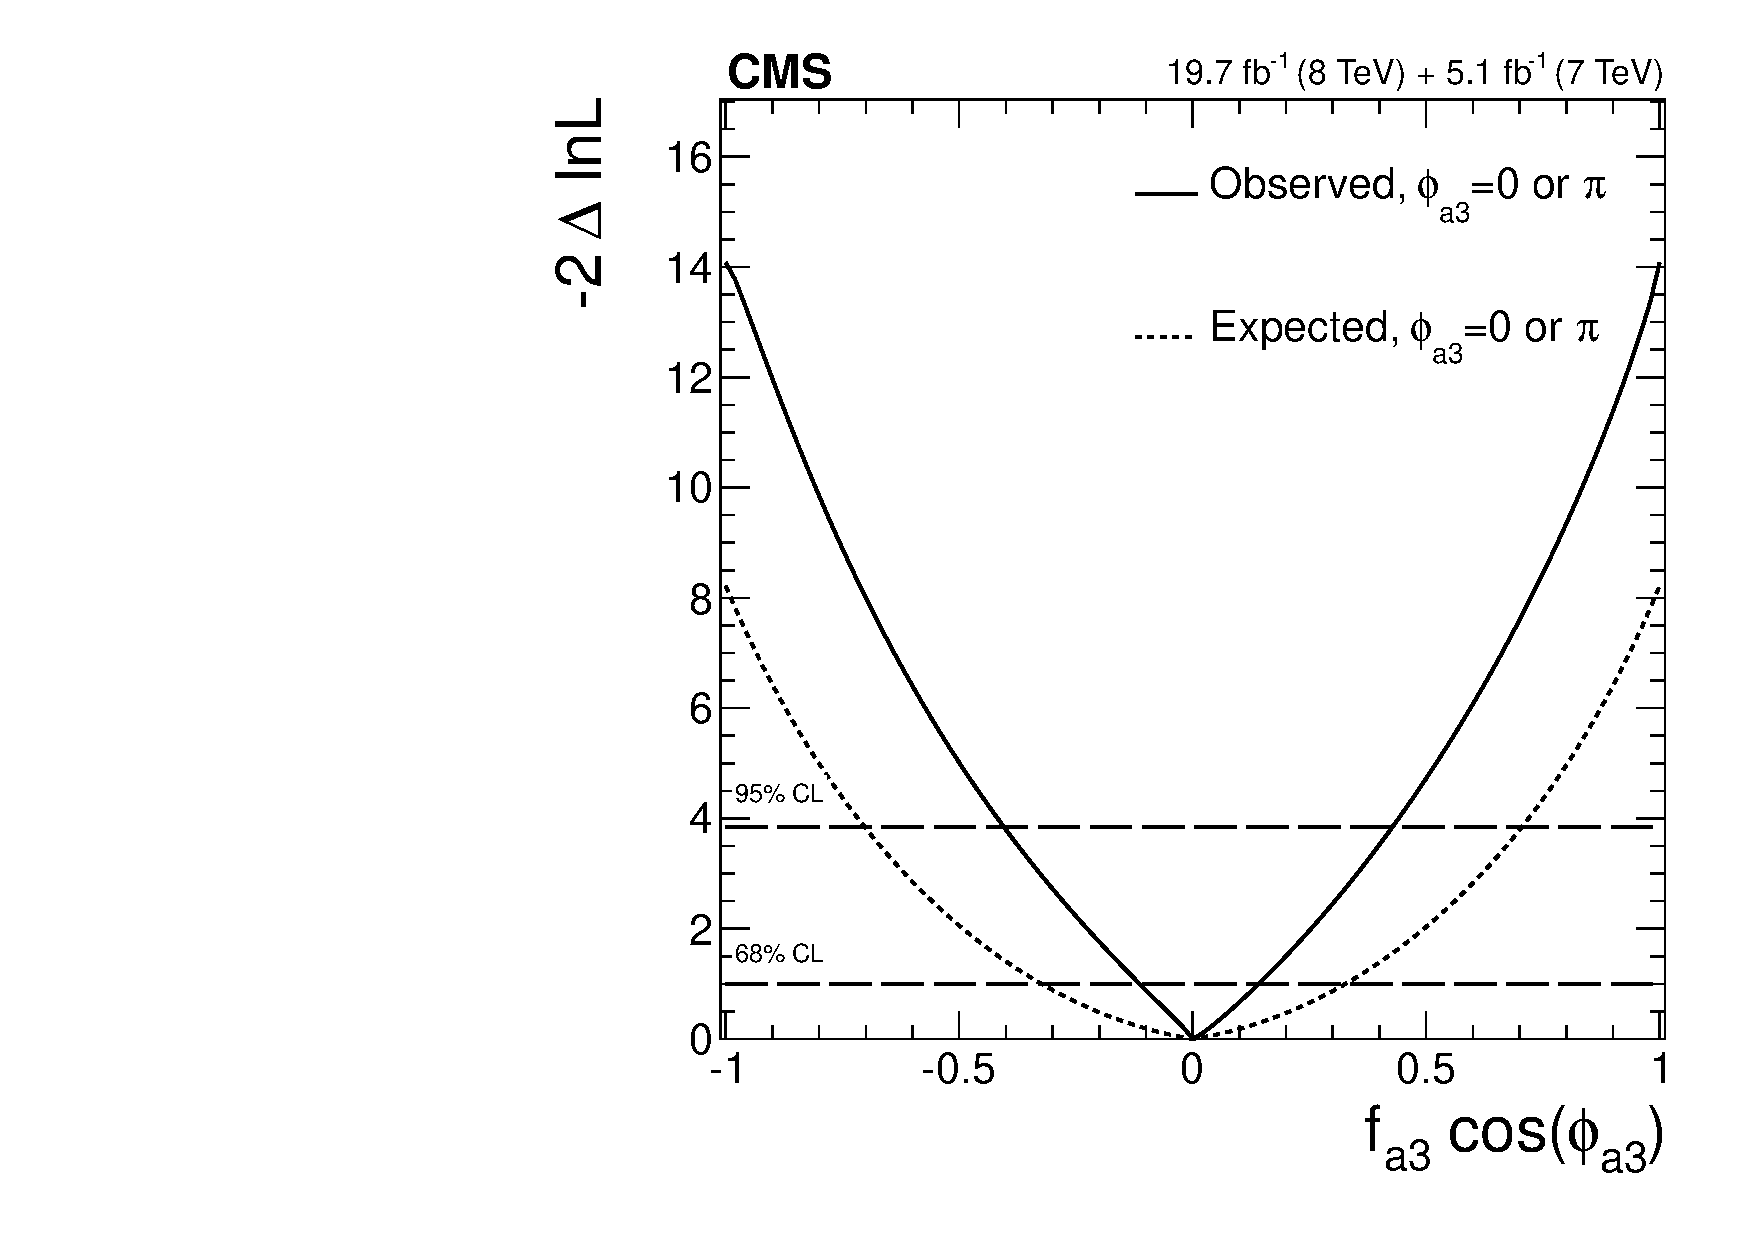
\includegraphics[width=0.38\textwidth]{Spin_Parity/fa3_Real.pdf}
       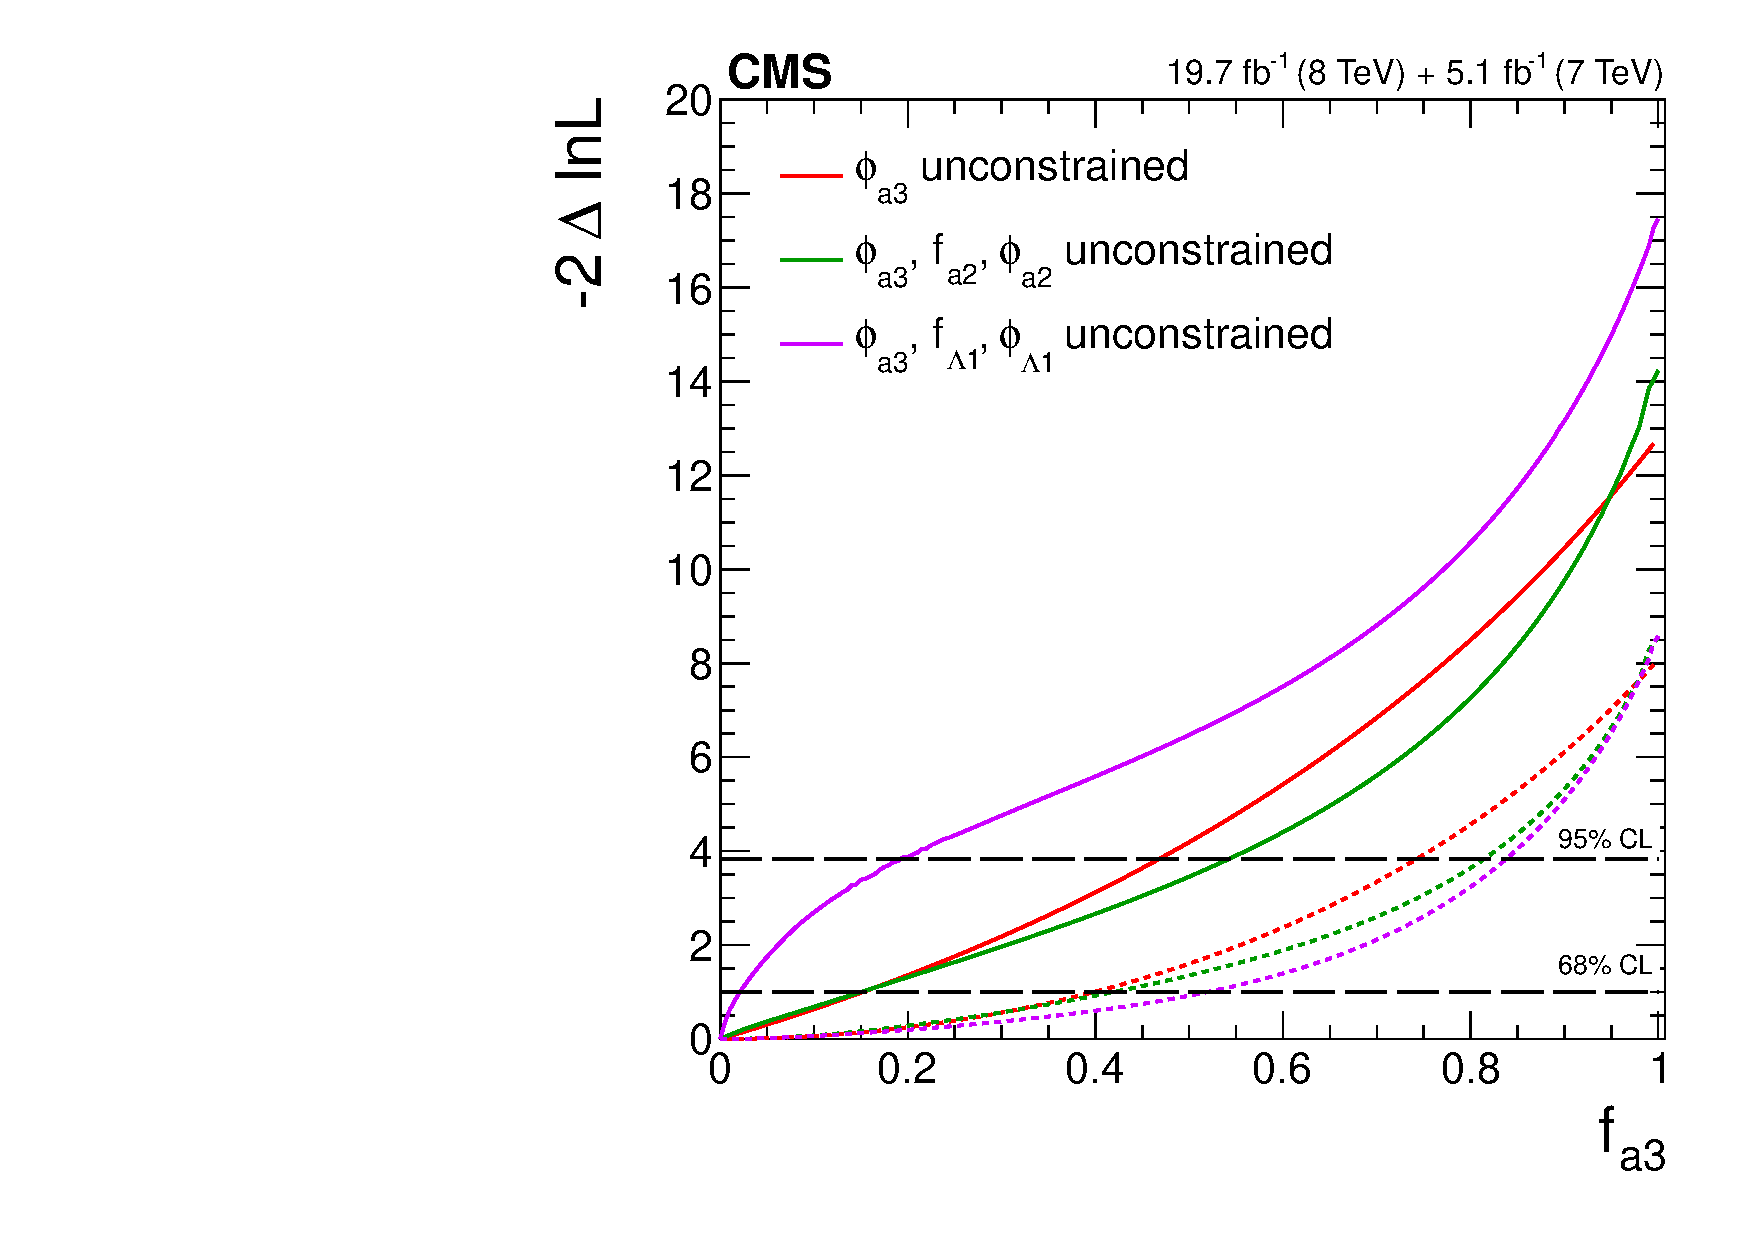
\includegraphics[width=0.38\textwidth]{Spin_Parity/fa3_Profile.pdf} \\
	\caption[Expected (dashed) and observed (solid) likelihood scans for
	the effective fractions $f_{\Lambda1}$, $f_{a2}$, $f_{a3}$ (from top to bottom) describing $HZZ$ interactions.
	Plots on the left show the results when the couplings studied are constrained to be real and all other couplings are fixed to the SM predictions.
	The $\cos\phi_{ai}$ term allows a signed quantity where $\cos\phi_{ai}=-1$ or $+1$.
	Plots on the right show the results where the phases of the anomalous couplings and
	additional $HZZ$ couplings are left unconstrained, as indicated in the legend.]{
	Expected (dashed) and observed (solid) likelihood scans for
	the effective fractions $f_{\Lambda1}$, $f_{a2}$, $f_{a3}$ (from top to bottom) describing $HZZ$ interactions.
	Plots on the left show the results when the couplings studied are constrained to be real and all other couplings are fixed to the SM predictions.
	The $\cos\phi_{ai}$ term allows a signed quantity where $\cos\phi_{ai}=-1$ or $+1$.
	Plots on the right show the results where the phases of the anomalous couplings and
	additional $HZZ$ couplings are left unconstrained, as indicated in the legend.
	The $f_{a3}$ result with $\phi_{a3}$ unconstrained (in the bottom-right plot) is from \cite{Chatrchyan:2013mxa} otherwise these results are from \cite{Khachatryan:2014kca}.
	}
	\label{fig:results_ZZ_1D}

\end{figure}

\begin{table}
\centering
\caption[Summary of the allowed 95\%~C.L. intervals on the anomalous couplings in $HZZ$ interactions
using results in table~\ref{tab:summary_spin0}.
The coupling ratios are assumed to be real (including $\cos(\phi_{\Lambda_{1}})=0$ or $\pi$).]{
Summary of the allowed 95\%~C.L. intervals on the anomalous couplings in $HZZ$ interactions
using results in table~\ref{tab:summary_spin0} \cite{Khachatryan:2014kca}.
The coupling ratios are assumed to be real (including $\cos(\phi_{\Lambda_{1}})=0$ or $\pi$).
\label{tab:Spin0zz_interpretation}
}
\begin{tabular}{cccccc}
Parameter  & Observed & Expected    \\
\hline

$(\Lambda_{1}\sqrt{\abs{a_1}}) \cos(\phi_{\Lambda_{1}})$ &   $[-\infty,-119\GeV]\cup[104\GeV,\infty]$ & $[-\infty,50\GeV] \cup [116\GeV,\infty]$                                            \\

$ a_{2}/a_{1} $ &   $[-2.28,-1.88]\cup[-0.69,\infty]$ & $[-0.77,\infty]$                                               \\

$ a_{3}/a_{1} $ &   $[-2.05,2.19]$ & $[-3.85,3.85]$                                               \\
\end{tabular}
\end{table}

\begin{figure}
\centering
	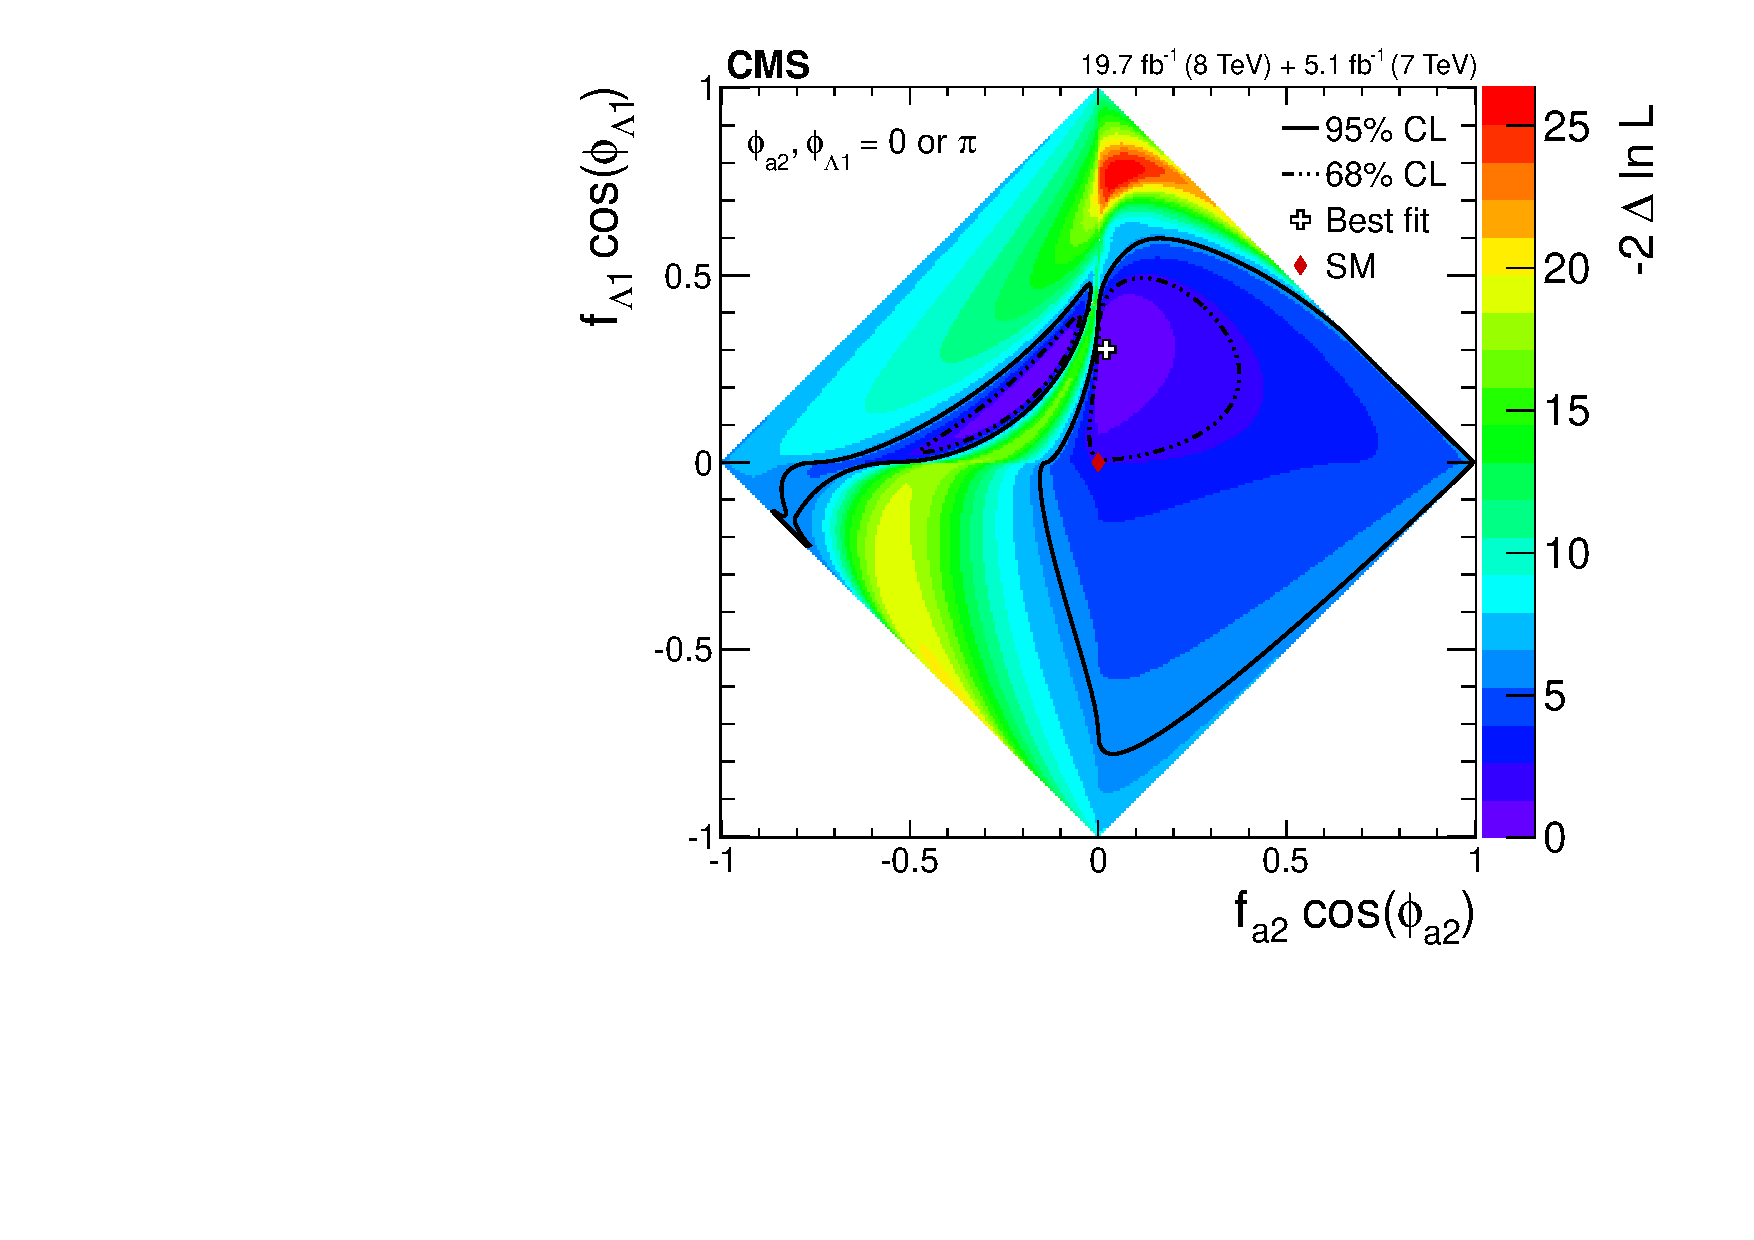
\includegraphics[width=0.45\textwidth]{Spin_Parity/fL1_vs_fa2_Real.pdf}
	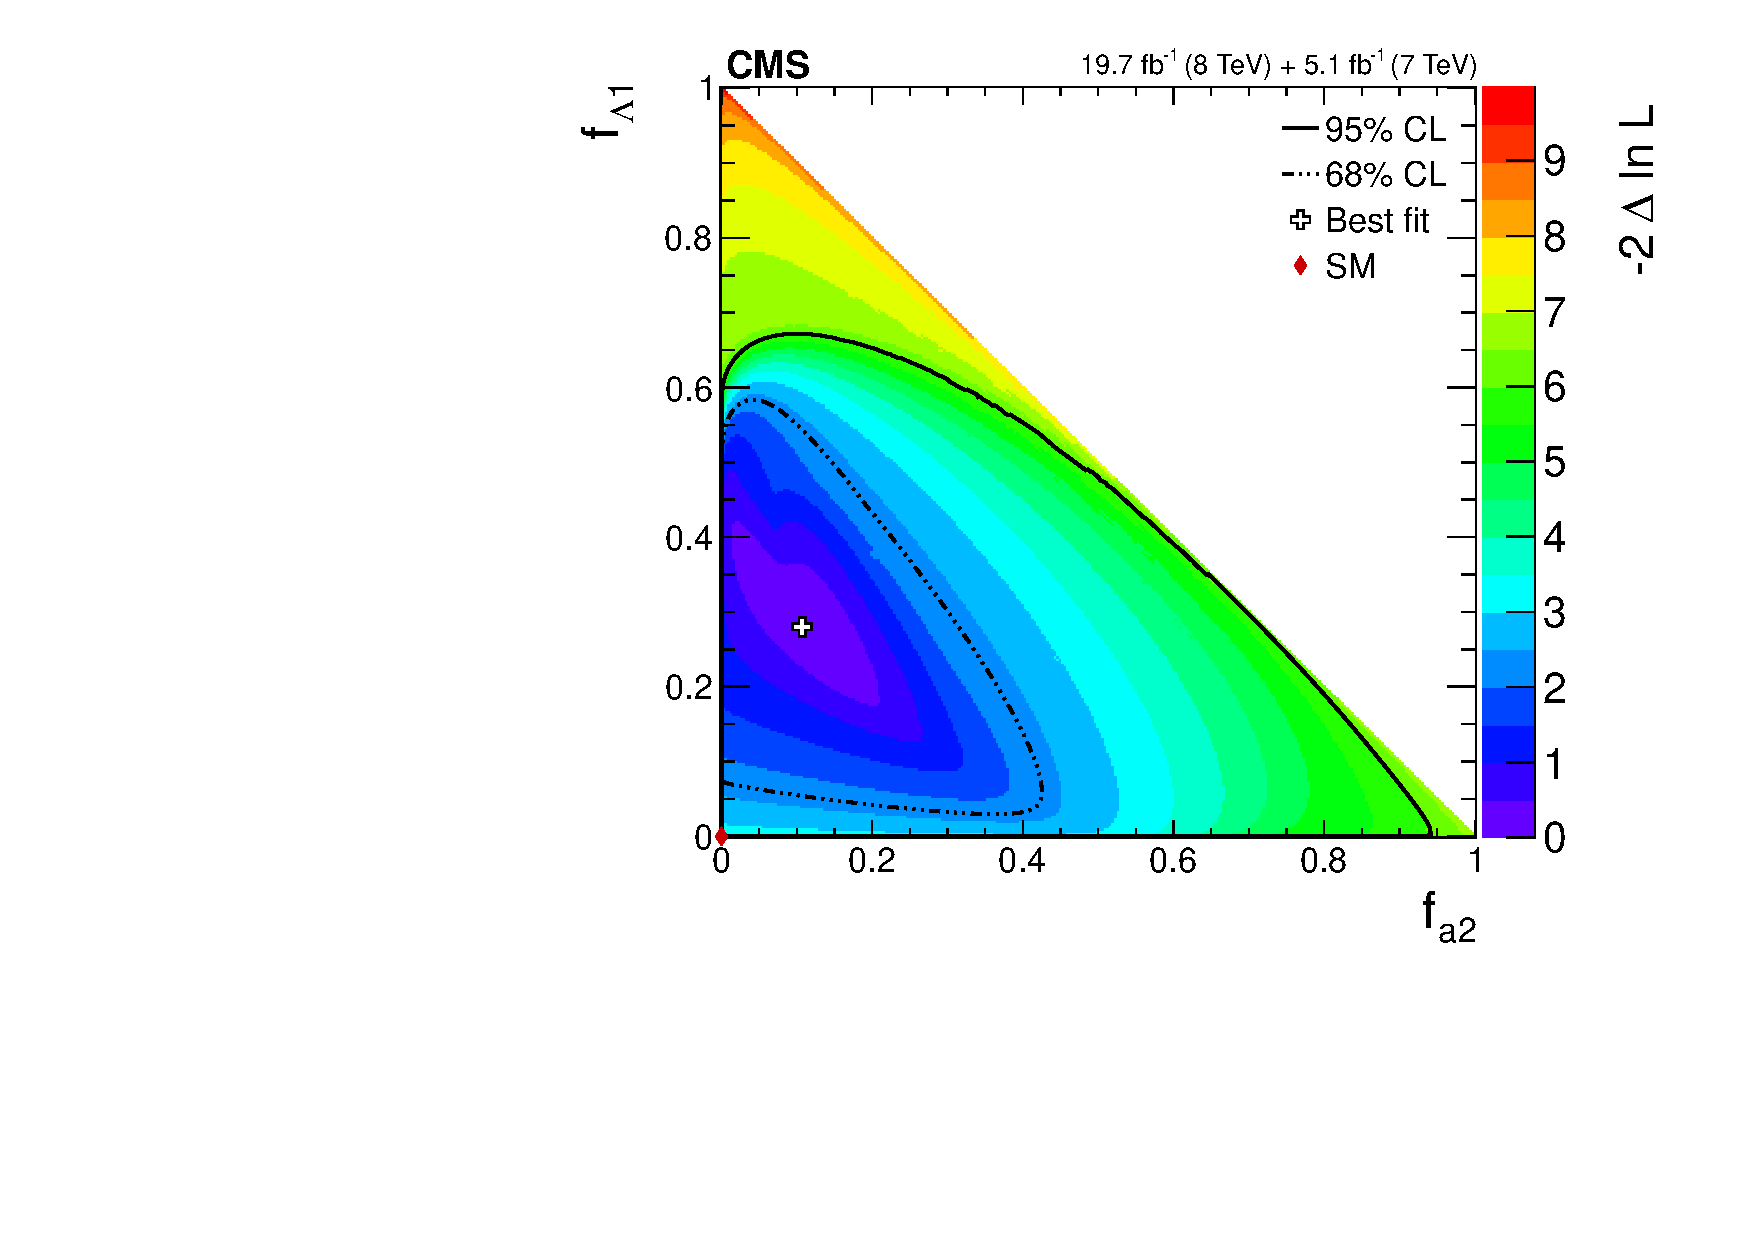
\includegraphics[width=0.45\textwidth]{Spin_Parity/fL1_vs_fa2_Profile.pdf} \\
	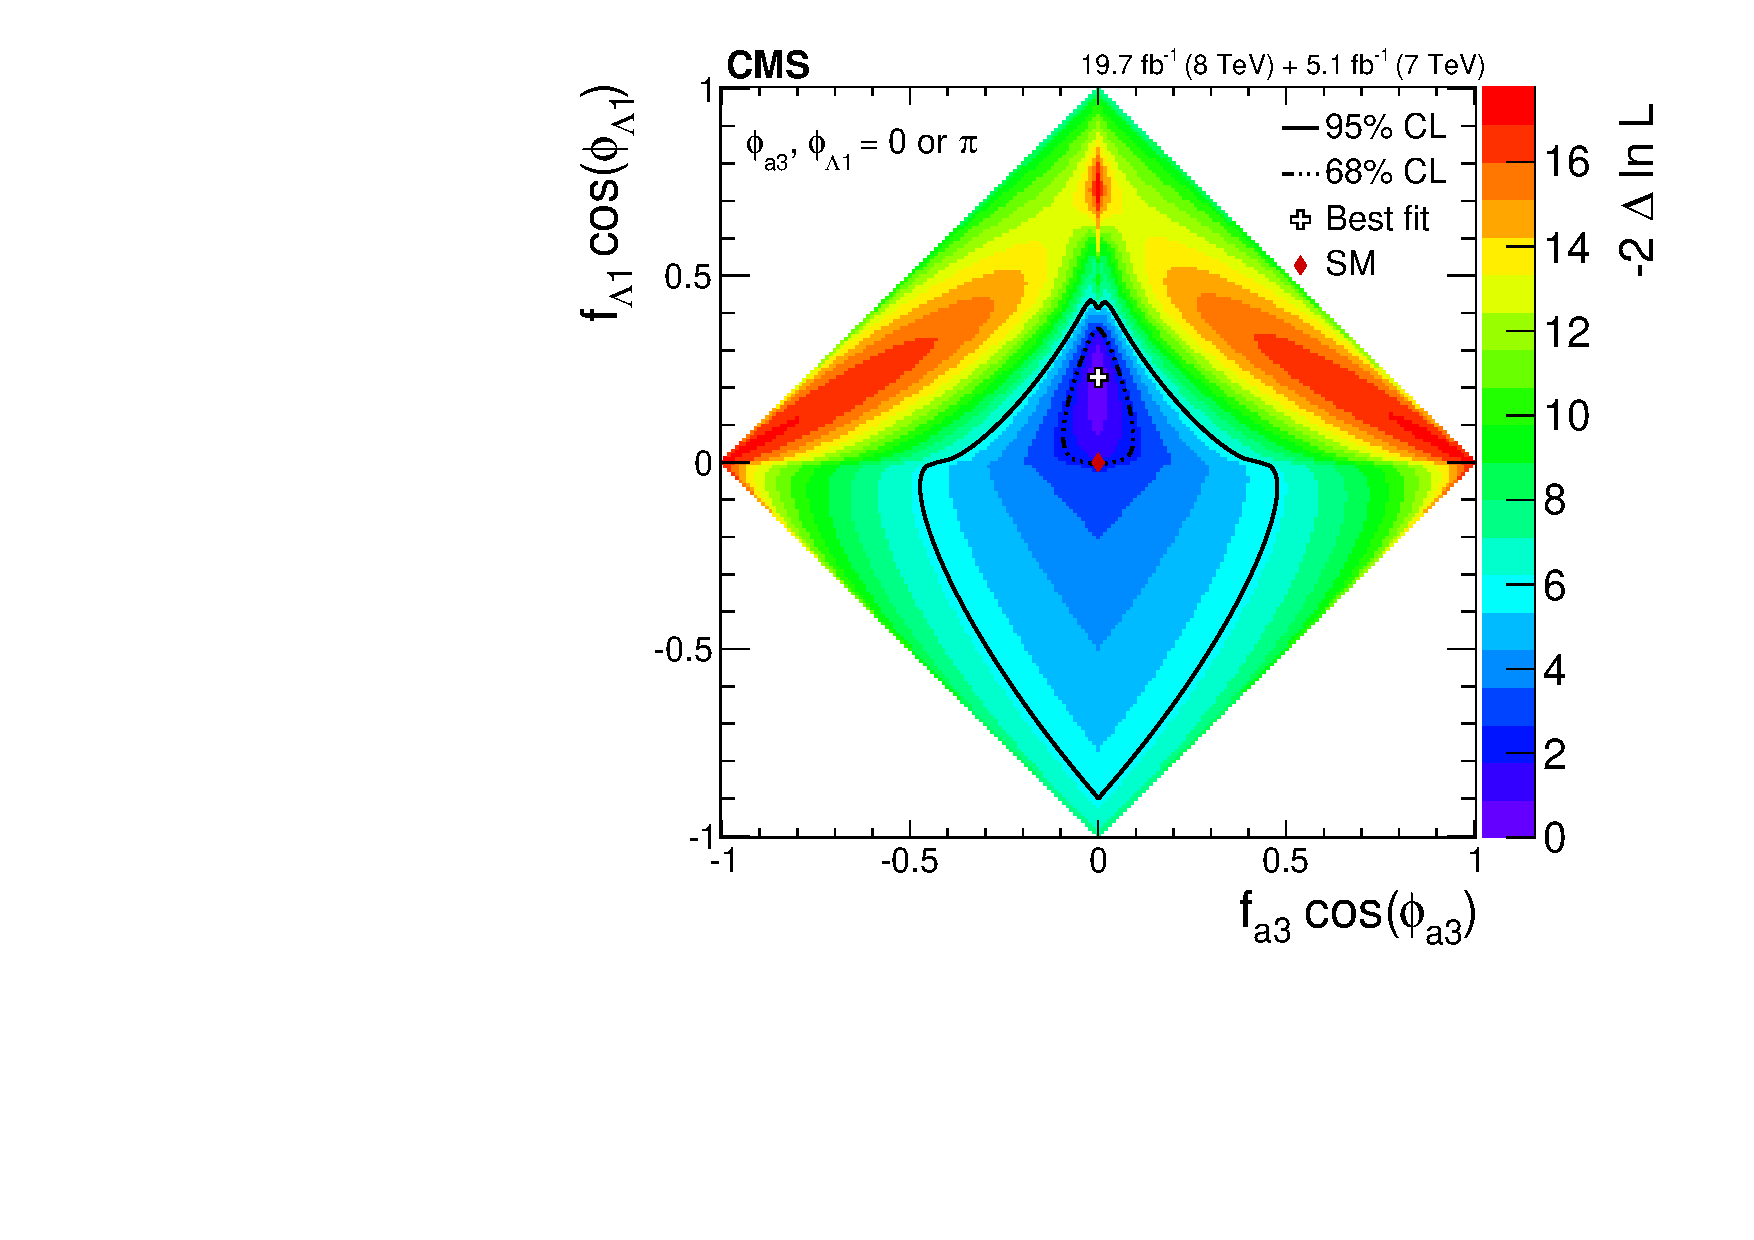
\includegraphics[width=0.45\textwidth]{Spin_Parity/fL1_vs_fa3_Real.pdf}
	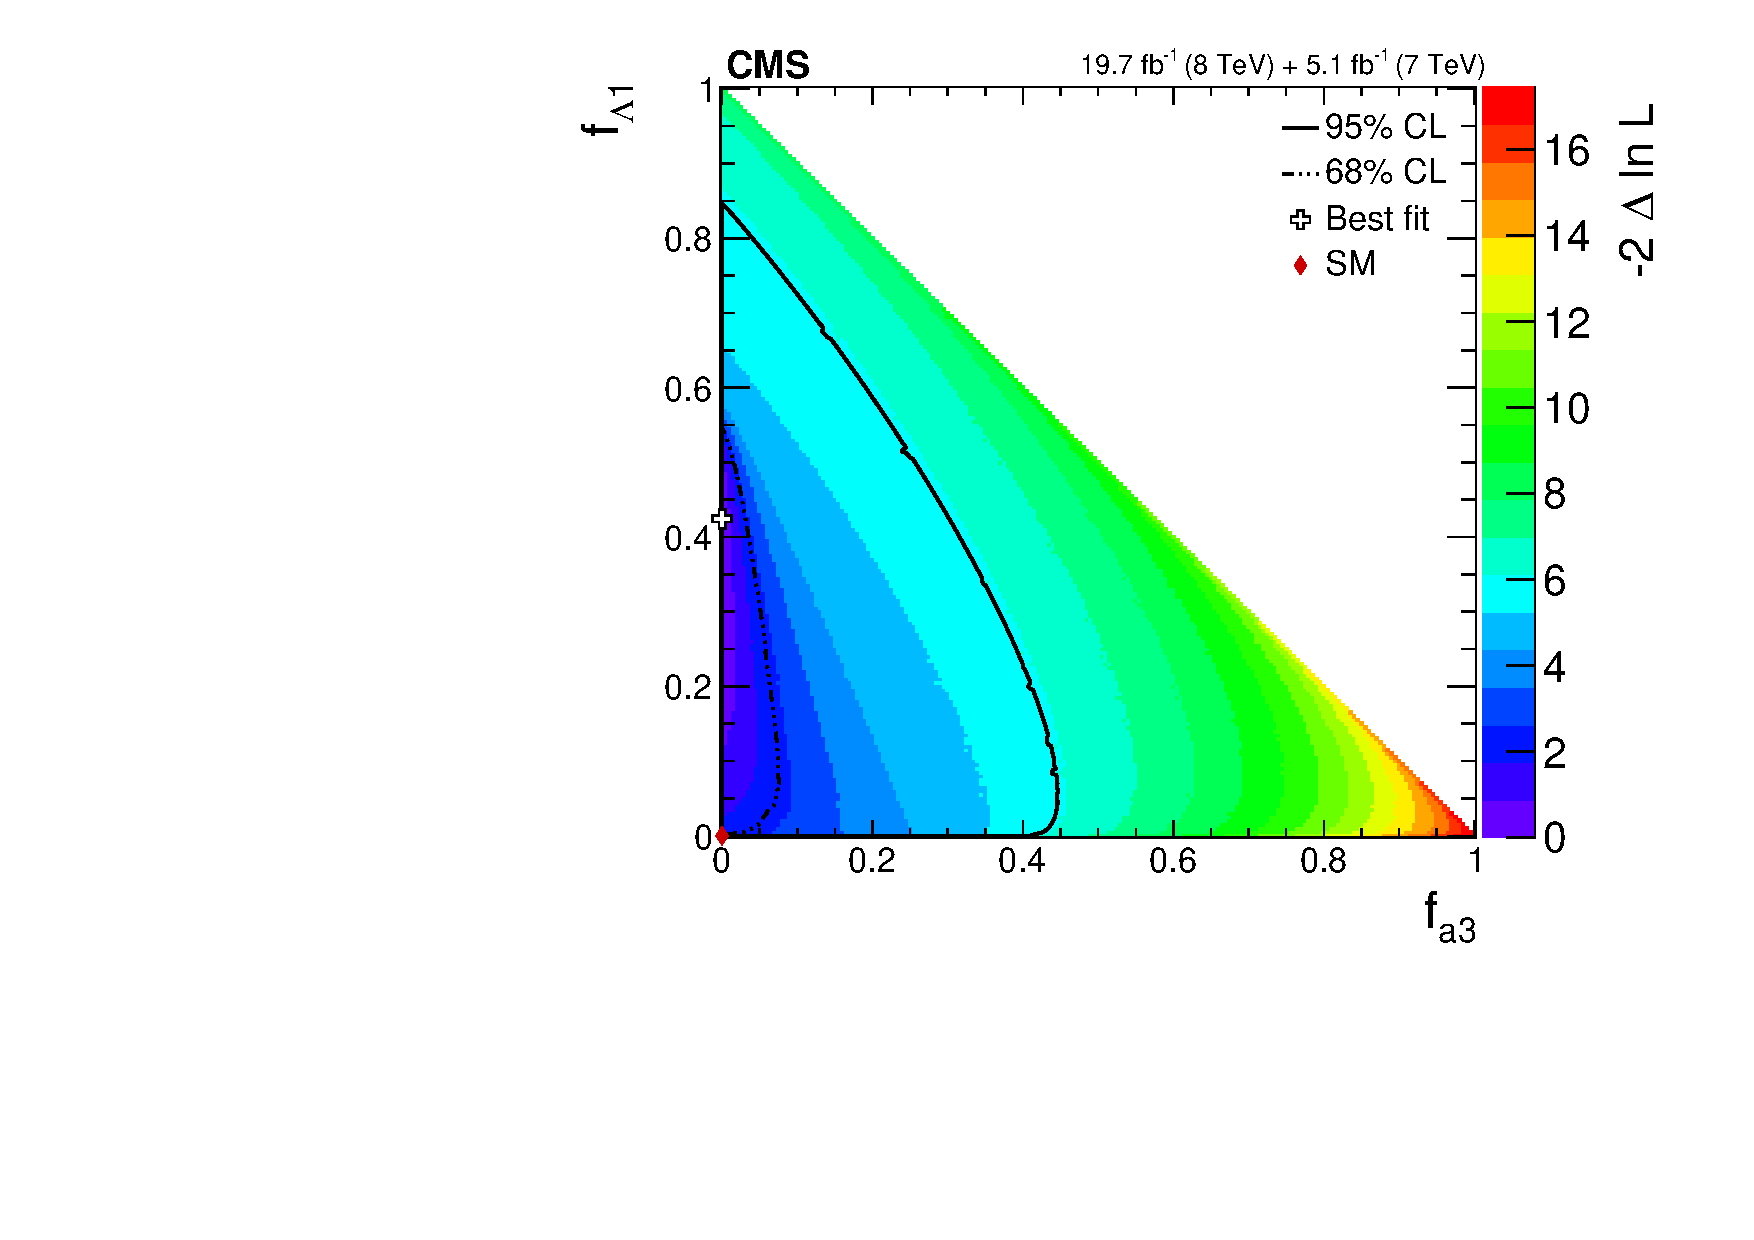
\includegraphics[width=0.45\textwidth]{Spin_Parity/fL1_vs_fa3_Profile.pdf}  \\
	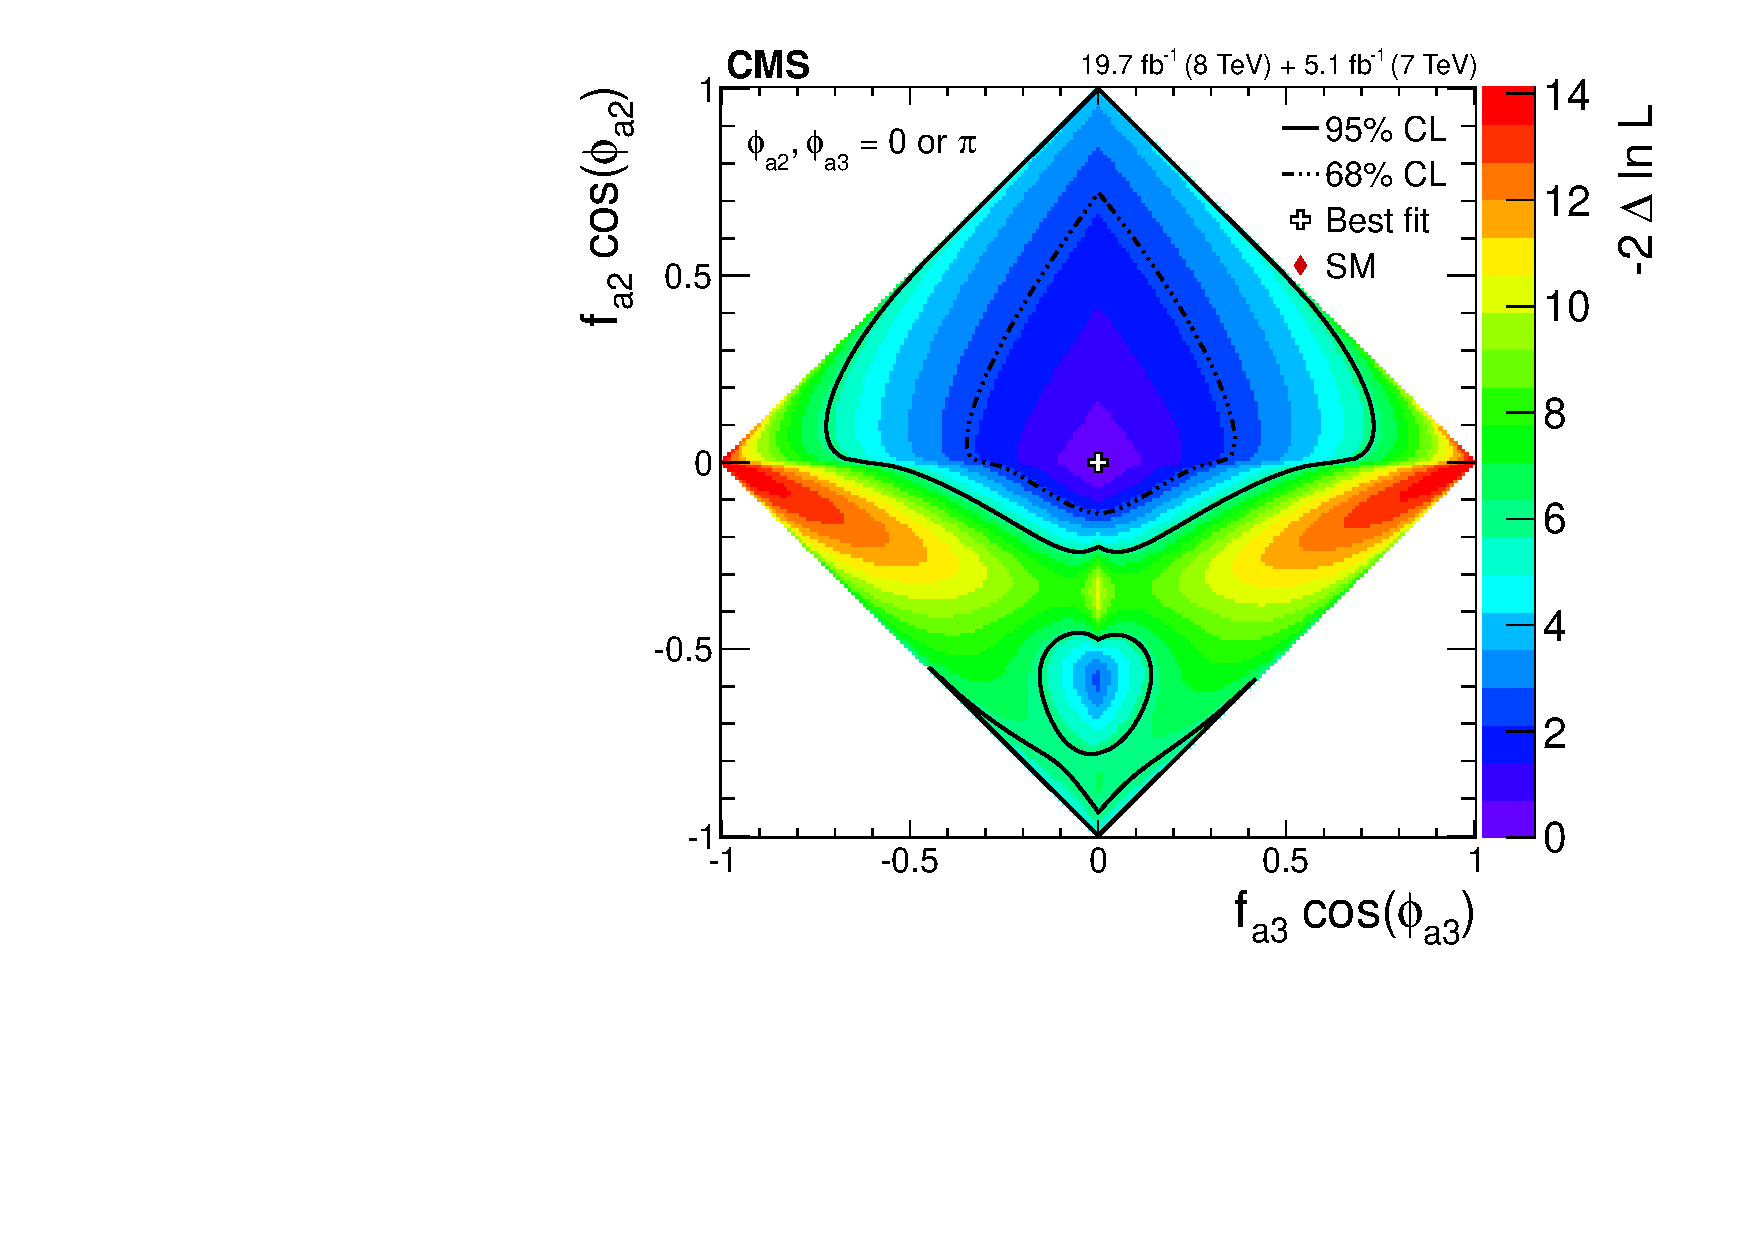
\includegraphics[width=0.45\textwidth]{Spin_Parity/fa2_vs_fa3_Real.pdf}
	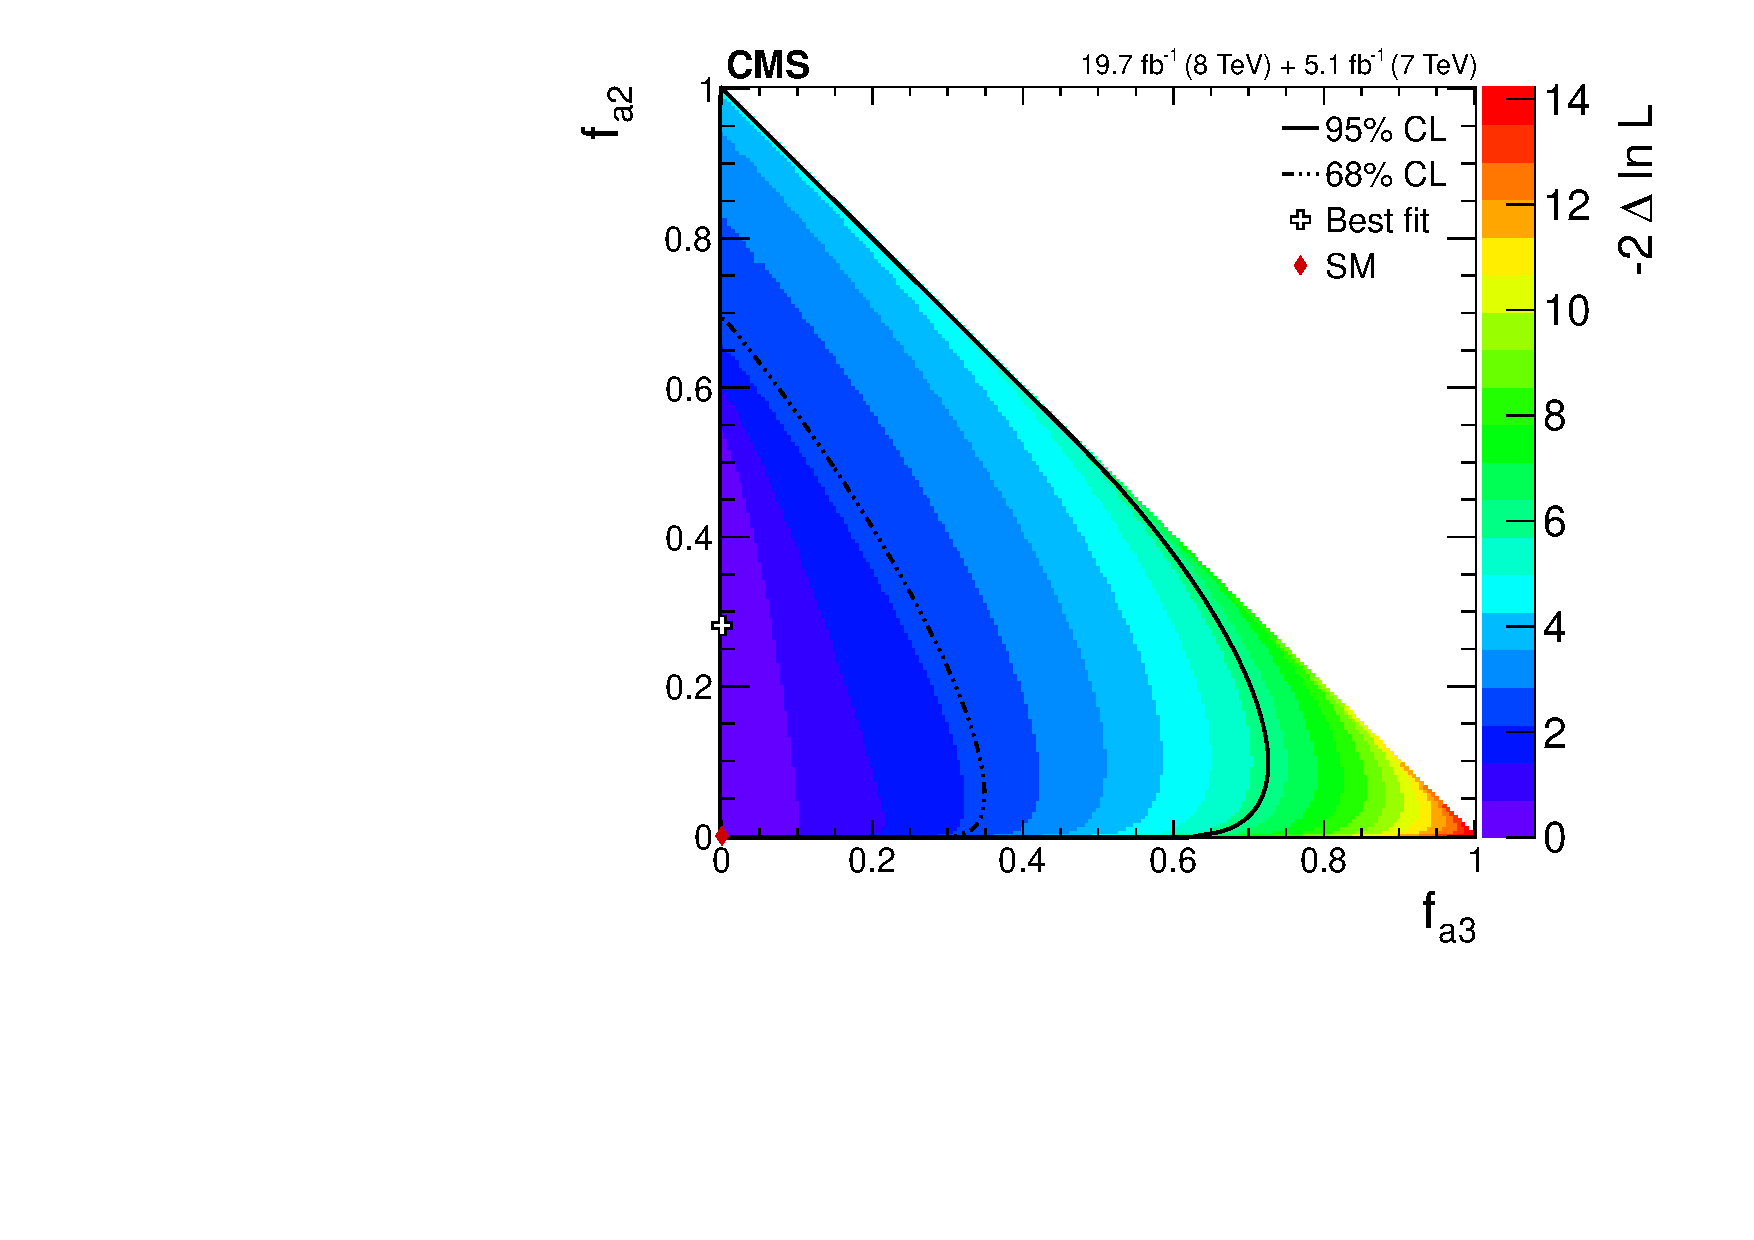
\includegraphics[width=0.45\textwidth]{Spin_Parity/fa2_vs_fa3_Profile.pdf}
	\caption[Observed likelihood scans for pairs of effective fractions $f_{\Lambda1}$ vs. $f_{a2}$,
	$f_{\Lambda1}$ vs. $f_{a3}$, and $f_{a2}$ vs. $f_{a3}$ (from top to bottom) describing $HZZ$ interactions.
	Plots on the left show the results when the couplings studied are constrained to be real
	and all other couplings are fixed to the SM predictions.
	Plots on the right show the results when the phases of the anomalous couplings are left unconstrained.
	The SM expectations correspond to points (0,0) and the best fit values are shown with the crosses.
	The confidence level intervals are indicated by the corresponding $-2\,\Delta\ln\mathcal{L}$ contours.]{
	Observed likelihood scans for pairs of effective fractions $f_{\Lambda1}$ vs. $f_{a2}$,
	$f_{\Lambda1}$ vs. $f_{a3}$, and $f_{a2}$ vs. $f_{a3}$ (from top to bottom) describing $HZZ$ interactions.
	Plots on the left show the results when the couplings studied are constrained to be real
	and all other couplings are fixed to the SM predictions.
	Plots on the right show the results when the phases of the anomalous couplings are left unconstrained.
	The SM expectations correspond to points (0,0) and the best fit values are shown with the crosses.
	The confidence level intervals are indicated by the corresponding $-2\,\Delta\ln\mathcal{L}$ contours \cite{Khachatryan:2014kca}.
	}
	\label{fig:results_ZZ_2D}

\end{figure}

The above one-parameter measurements, with other couplings also considered to be unconstrained, are obtained
from the fit configurations used for the two-parameter measurements shown in figure~\ref{fig:results_ZZ_2D}.
Both options are considered, either with or without the assumption that the couplings are real. To simplify the analysis
the number of observables is kept to a maximum of three, the following discriminants are
used to set the constraints,
($\mathcal{D}_\text{bkg}$, $\mathcal{D}_{\Lambda1}$, $\mathcal{D}_{0h+}$),
($\mathcal{D}_\text{bkg}$, $\mathcal{D}_{\Lambda1}$, $\mathcal{D}_{0-}$),
and ($\mathcal{D}_\text{bkg}$, $\mathcal{D}_{0-}$ or $\mathcal{D}_{0h+}$),
for the measurements of
$f_{\Lambda1}$ vs. $f_{a2}$, $f_{\Lambda1}$ vs. $f_{a3}$, and $f_{a2}$ vs. $f_{a3}$, respectively.
The left set of plots in figure \ref{fig:results_ZZ_2D} shows constraints on two real couplings, and
the right set of plots in figure \ref{fig:results_ZZ_2D} shows constraints on two couplings that are
allowed to have any complex phase. Similarly to the one-parameter constraints,
the allowed 95\% C.L. regions are formally defined using the profile likelihood function ($-2\Delta \ln\mathcal{L} = 5.99$).
The results in Table~\ref{tab:Spin0_ZZ_1D_KDb} are obtained from these two-parameter likelihood scans by profiling one parameter.

Overall, all anomalous $HZZ$ couplings are found to be consistent with zero, which is also consistent with the expectation
from the SM where these couplings are expected to be very small, well below the current sensitivity.

\begin{table}
\centering
\caption[Summary of the allowed 68\%~C.L. (central values with uncertainties) and 95\%~C.L. (ranges in square brackets)
intervals on anomalous coupling parameters in the $HZZ$ interactions under the condition of a given phase of
the coupling (0 or $\pi$) or when the phase or other parameters are unconstrained (any value allowed).
Expectations are quoted in parentheses following the observed values. ]{
Summary of the allowed 68\%~C.L. (central values with uncertainties) and 95\%~C.L. (ranges in square brackets)
intervals on anomalous coupling parameters in the $HZZ$ interactions under the condition of a given phase of
the coupling (0 or $\pi$) or when the phase or other parameters are unconstrained (any value allowed).
Expectations are quoted in parentheses following the observed values. The results for $f_{a3}$ with $\phi_{a3}$ unconstrained are from~\cite{Chatrchyan:2013mxa} while the other results are form \cite{Khachatryan:2014kca}.
}
\begin{tabular}{lccc}
Measurement              &  $f_{\Lambda1}$ &  $f_{a2}$  & $f_{a3}$    \\
\hline \hline
 $\phi_{ai}=0$
 &   $0.22^{+0.10}_{-0.16}$ $[0.00,0.37]$ &   $0.00^{+0.42}_{-0.00}$ $[0.00,1.00]$ & $0.00^{+0.14}_{-0.00}$ $[0.00,0.43]$  \\
 &   (~$0.00^{+0.16}_{-0.00}$ $[0.00,0.27]$ &   (~$0.00^{+0.35}_{-0.00}$ $[0.00,1.00]$~) & (~$0.00^{+0.33}_{-0.00}$ $[0.00,0.70]$~)  \\
 &   ~~~~~~~~~~~~~~~~$\cup [0.92,1.00]$~) &  &  \\ \hline
 $\phi_{ai}=\pi$
 &  $0.00^{+0.08}_{-0.00}$ $[0.00,0.82]$ &   $0.00^{+0.06}_{-0.00}$ $[0.00,0.15]$ &   $0.00^{+0.11}_{-0.00}$ $[0.00,0.40]$  \\
 &   &  ~~~~~~~~~~~~~~~$\cup [0.56,0.68]$ &    \\
 &   (~$0.00^{+0.87}_{-0.00}$ $[0.00,1.00]$~) &   (~$0.00^{+0.08}_{-0.00}$ $[0.00,0.18]$ & (~$0.00^{+0.32}_{-0.00}$ $[0.00,0.70]$~)  \\
 &  &   $~~~~~~~~~~~~~~~~\cup [0.62,0.73]$~) &  \\ \hline
  any $\phi_{ai}$
 &  $0.39^{+0.16}_{-0.31}$ $[0.00,0.57]$ &   $0.32^{+0.28}_{-0.32}$ $ [0.00,1.00]$ &   $0.00^{+0.17}_{-0.00}$  $[0.00,0.47]$  \\
 &   (~$0.00^{+0.85}_{-0.00}$ $[0.00,1.00]$~) &   (~$0.00^{+0.59}_{-0.00}$ $[0.00,1.00]$~) & (~$0.00^{+0.40}_{-0.00}$ $[0.00,0.74]$~)  \\ \hline
any $\phi_{ai}$,
&   ~~~~ &   $0.11^{+0.16}_{-0.11}$ $[0.00,0.65]$ &   $0.00^{+0.02}_{-0.00}$ $[0.00,0.19]$  \\
$f_{\Lambda1},\phi_{\Lambda1}$&   ~~~~  &   (~$0.00^{+0.72}_{-0.00}$ $[0.00,1.00]$~) &(~$0.00^{+0.52}_{-0.00}$ $[0.00,0.84]$~)  \\ \hline
any $\phi_{ai}$,
 &  $0.28^{+0.21}_{-0.15}$ $[0.00,0.63]$ &    ~~~~ &   $0.00^{+0.15}_{-0.00}$ $[0.00,0.54]$  \\
$f_{a2},\phi_{a2}$&   (~$0.00^{+0.85}_{-0.00}$ $[0.00,1.00]$~) &   ~~~~ & (~$0.00^{+0.42}_{-0.00}$ $[0.00,0.81]$~)  \\ \hline
any $\phi_{ai}$,
&  $0.42^{+0.09}_{-0.33}$ $[0.00,0.57]$ &   $0.28^{+0.29}_{-0.28}$ $[0.00,0.97]$ &    ~~~~  \\
$f_{a3},\phi_{a3}$&   (~$0.00^{+0.86}_{-0.00}$ $[0.00,1.00]$~) &   (~$0.00^{+0.59}_{-0.00}$ $[0.00,1.00]$~) & ~~~~  \\
\end{tabular}
\label{tab:Spin0_ZZ_1D_KDb}
\end{table}


\subsubsection{Study of $HZ\gamma$ and $H\gamma\gamma$ couplings with the $H\to VV\to4\ell$ channel}  \label{sec:Resultspinzerohzg}

In the following, constraints on anomalous $HZ\gamma$ and $H\gamma\gamma$ interactions
are obtained using the $H\to VV\to 4\ell$ data. Five anomalous couplings are considered,
following equation \eqref{eq:formfact-fullampl-spin0} and table~\ref{tab:kdlist}, where the three
observables for each measurement are listed. Only real couplings, $\phi_{ai}=0$ or $\pi$,
are considered in this test. The results of the likelihood function scan for the three parameters,
$f_{ai}\cos\phi_{ai}$, are shown in figure~\ref{fig:results_ZA_AA_1D}, following the same
formalism presented for the $HZZ$ couplings in section~\ref{sec:Resultspinzerohzz}.
The 68\% and 95\%~C.L. intervals are shown in table~\ref{tab:summary_spin0}.
In the case of the $f_{\Lambda1}^{Z\gamma}$ measurement, there are two minima and only
one central value with its 68\%~C.L. interval is shown in table~\ref{tab:summary_spin0},
while both 68\%~C.L. intervals are presented in figure \ref{fig:spin0_summary}.

\begin{figure}
\centering
	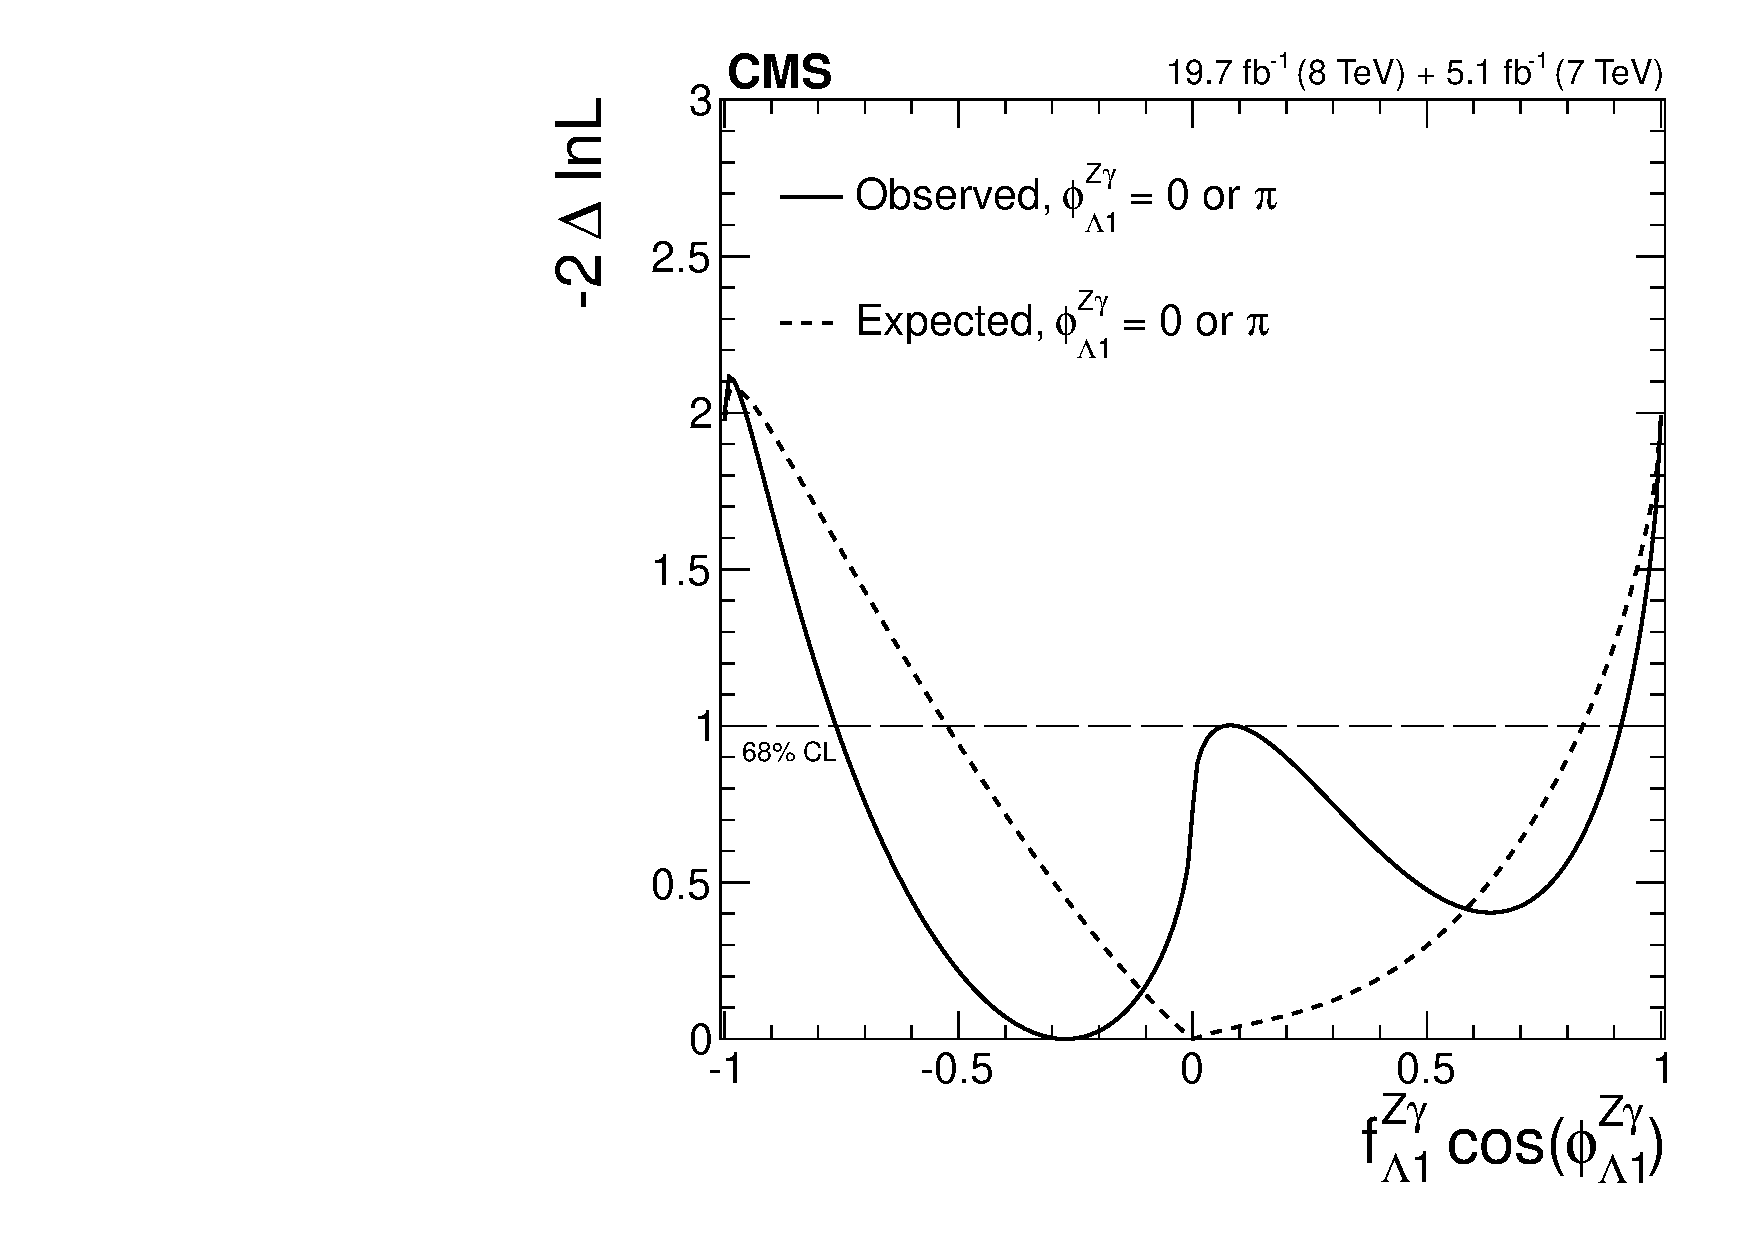
\includegraphics[width=0.38\textwidth,angle=0]{Spin_Parity/ZGamma_fL1.pdf} \\
	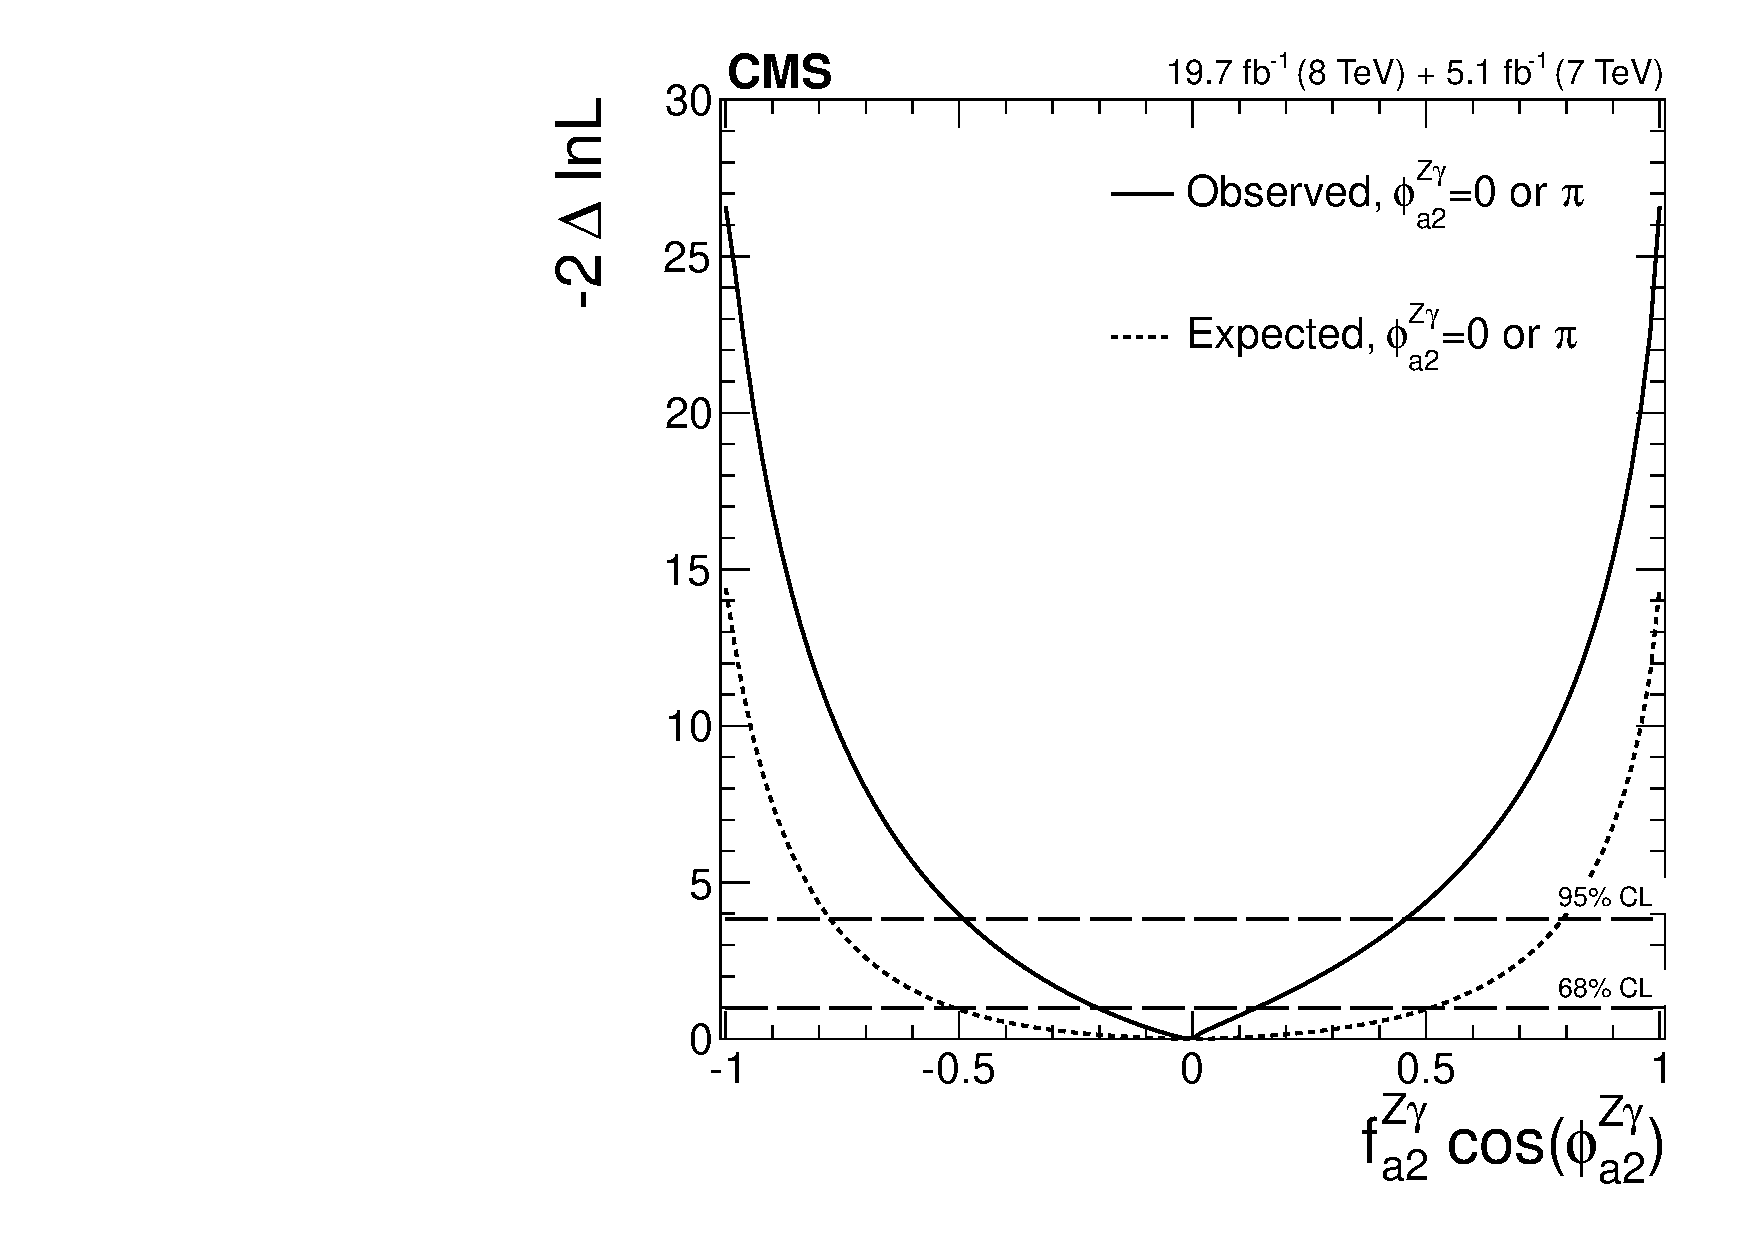
\includegraphics[width=0.38\textwidth,angle=0]{Spin_Parity/ZGamma_fa2.pdf}
	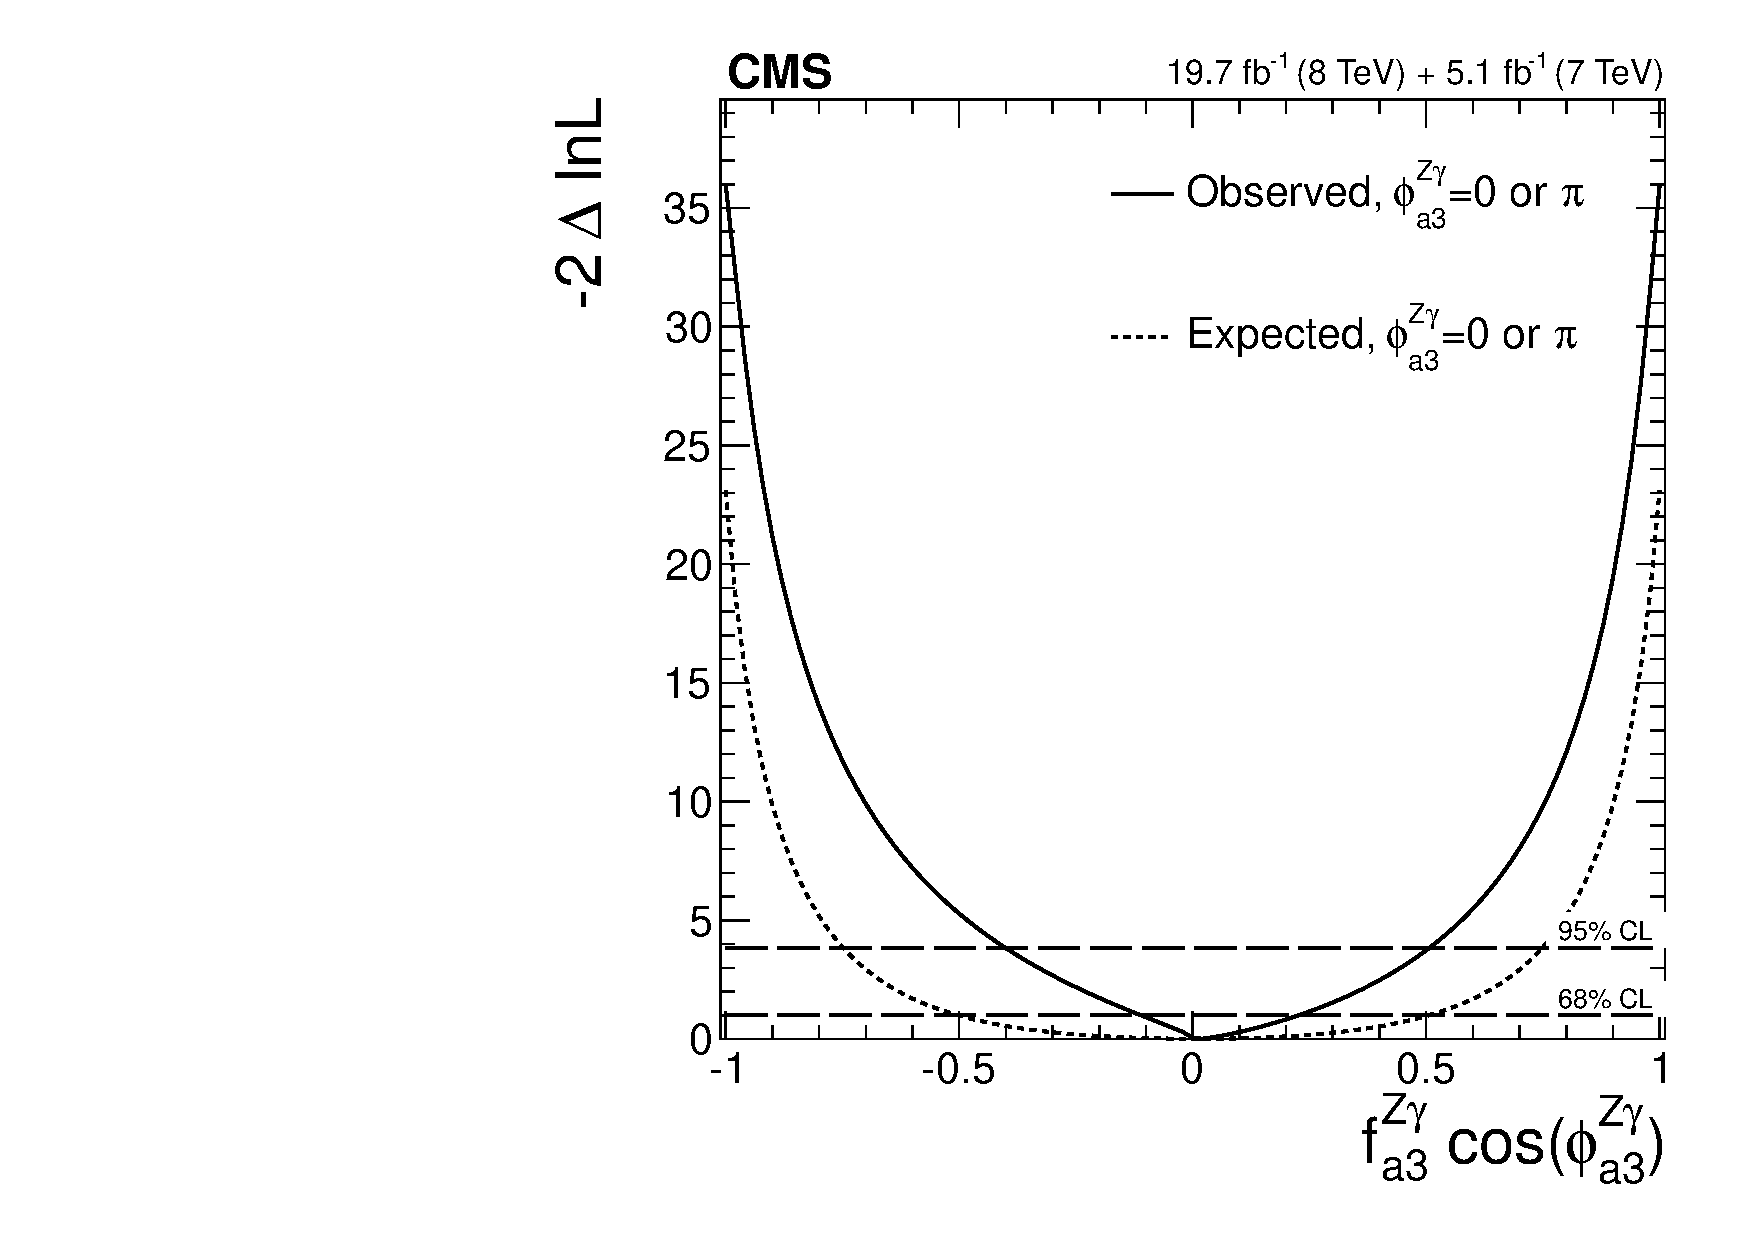
\includegraphics[width=0.38\textwidth,angle=0]{Spin_Parity/ZGamma_fa3.pdf} \\
	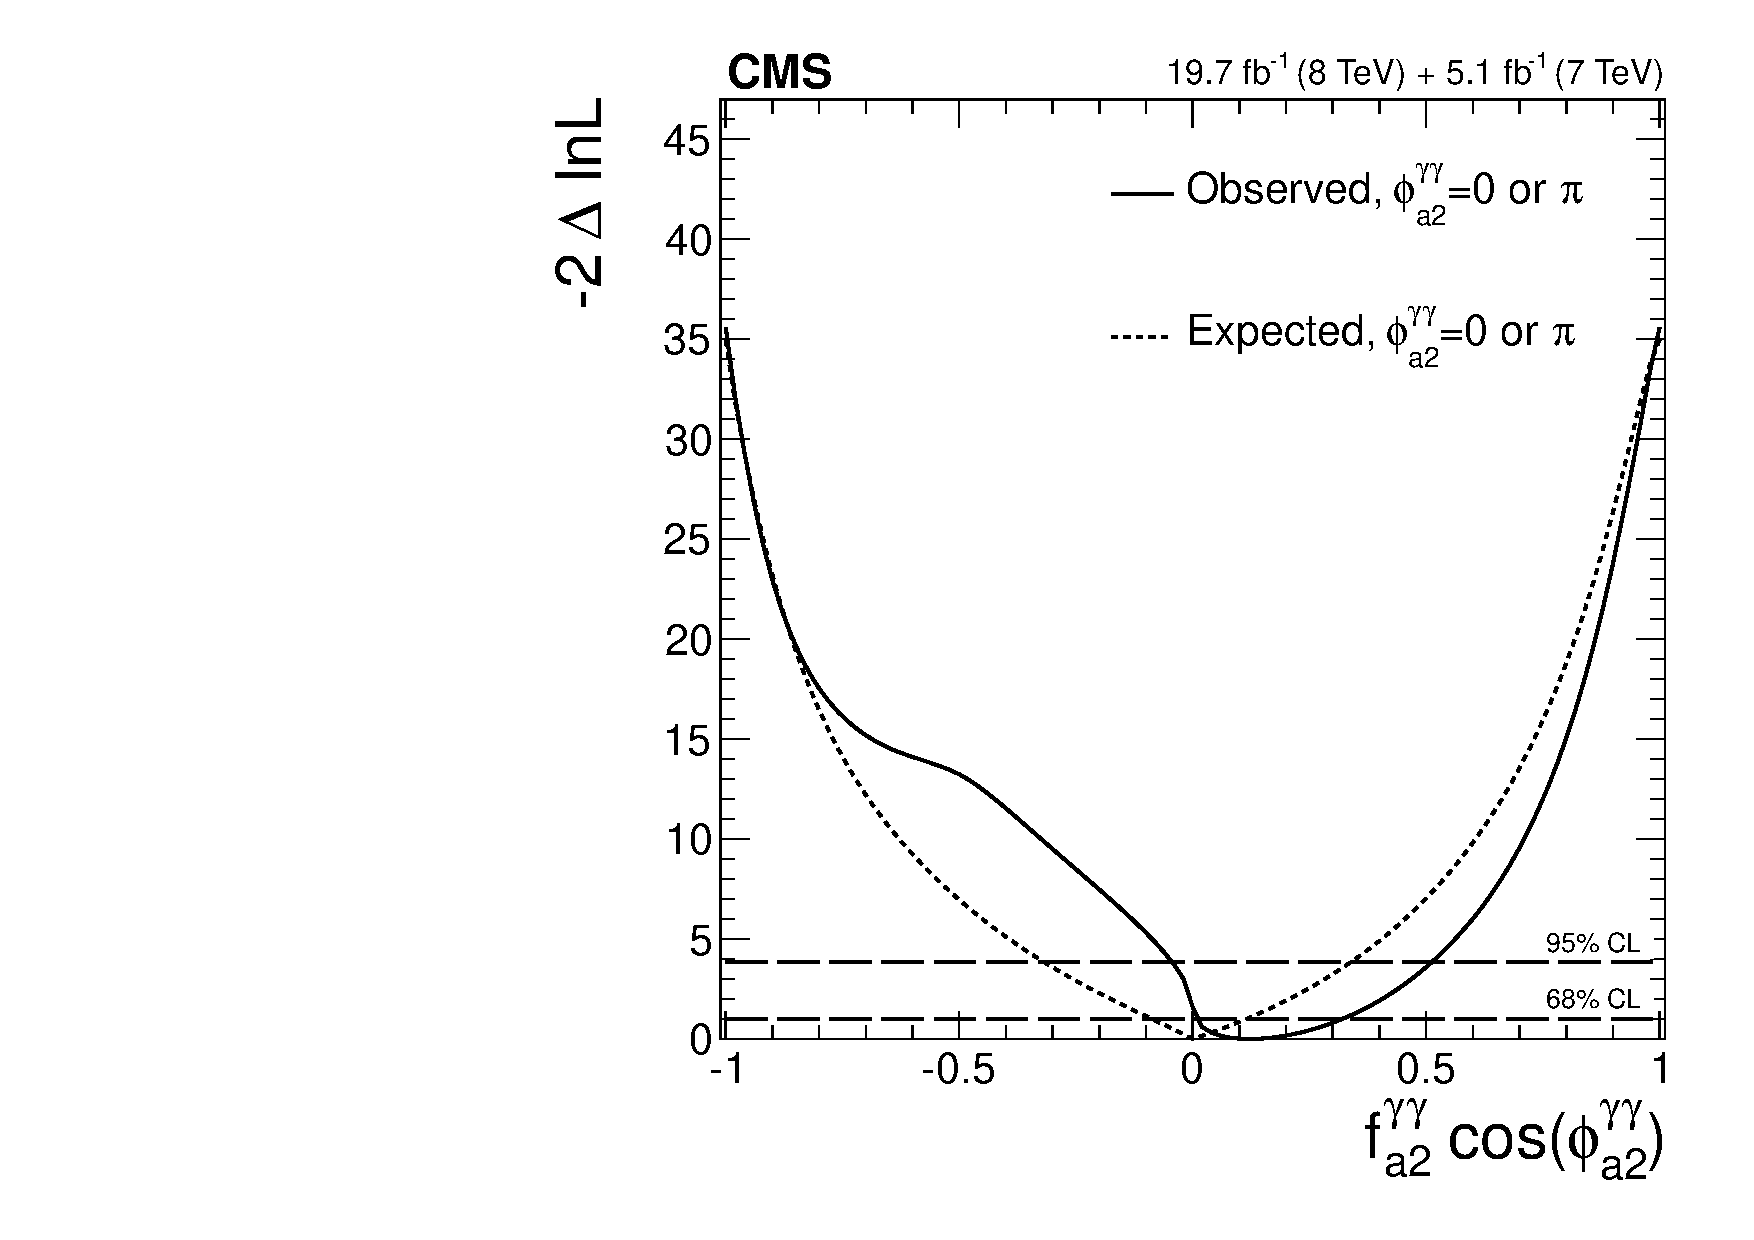
\includegraphics[width=0.38\textwidth,angle=0]{Spin_Parity/GammaGamma_fa2.pdf}
	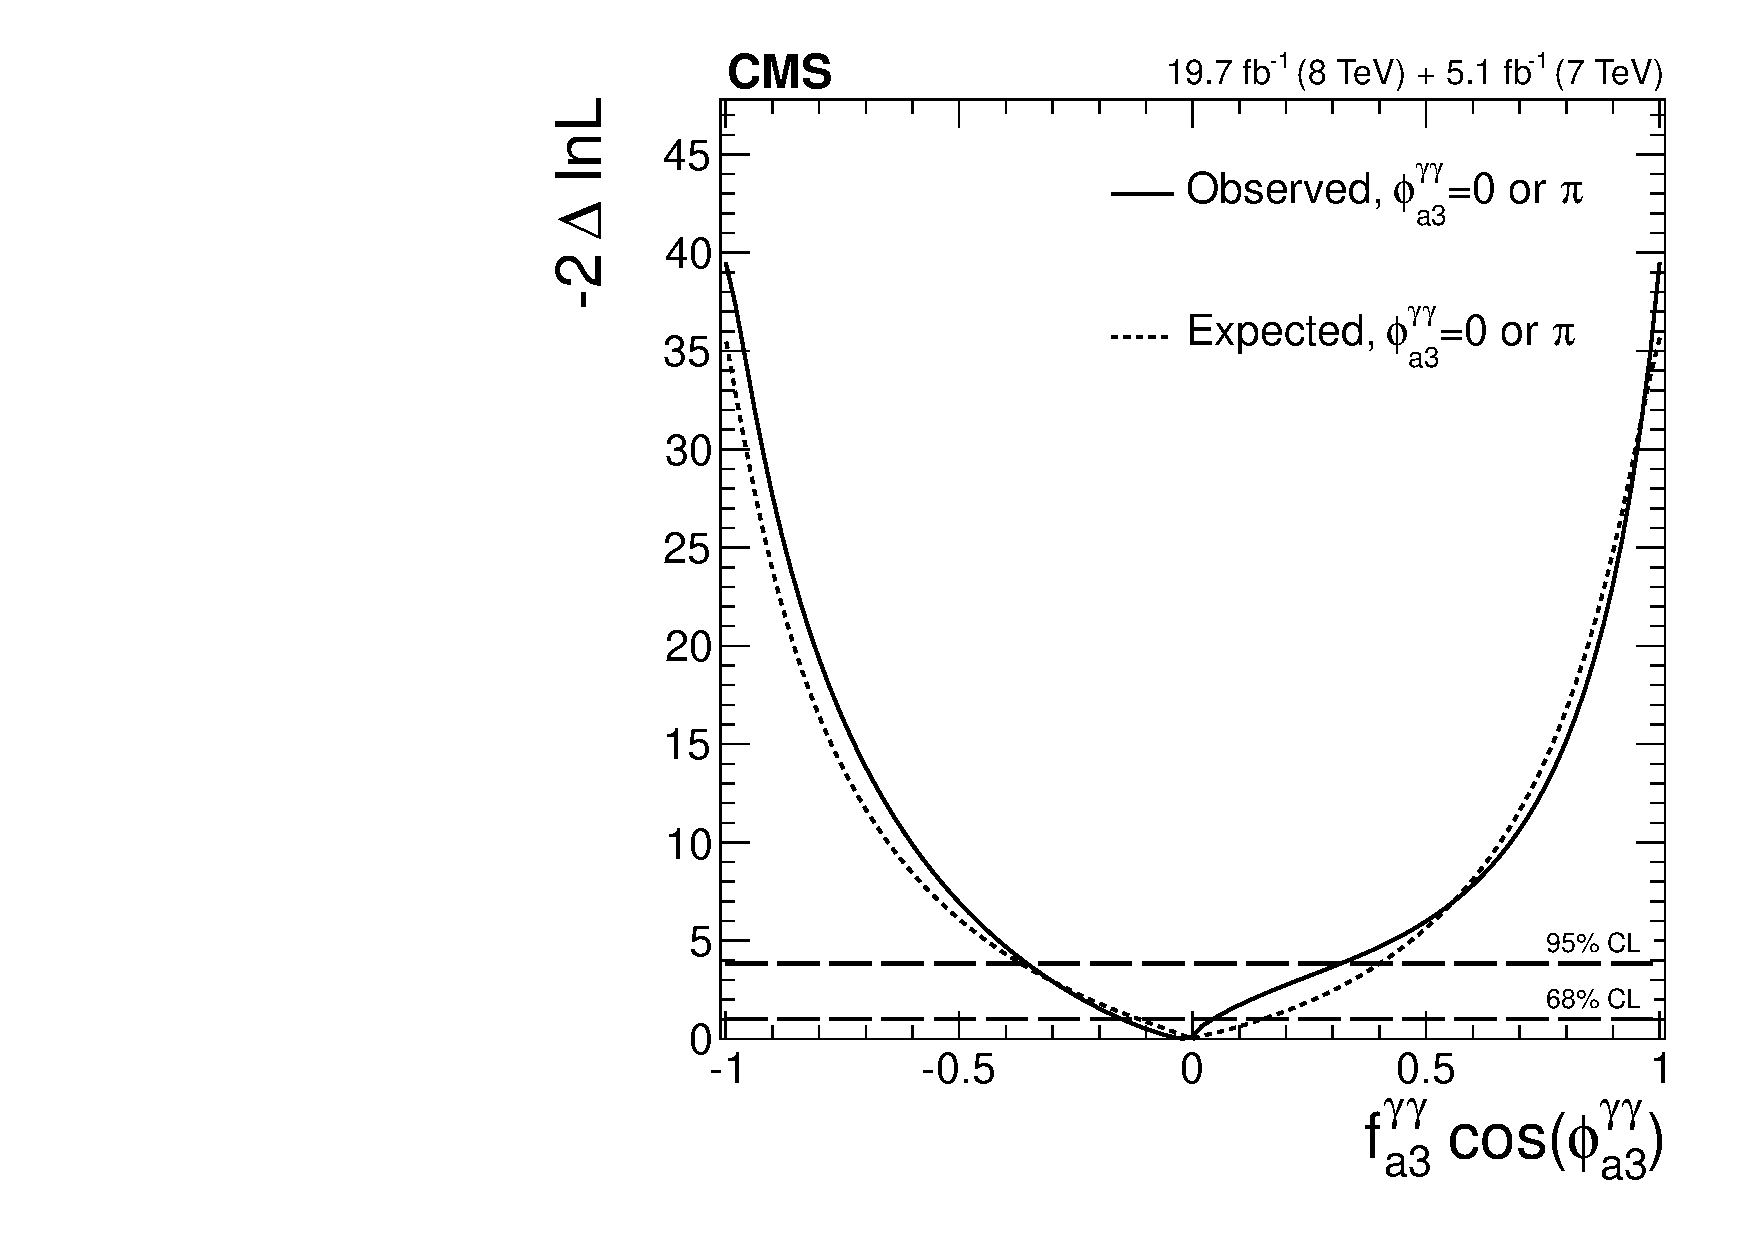
\includegraphics[width=0.38\textwidth,angle=0]{Spin_Parity/GammaGamma_fa3.pdf}
	\caption[Expected (dashed) and observed (solid)  likelihood scans for the effective fractions
	$f_{\Lambda1}^{Z\gamma}$ (top), $f_{a2}^{Z\gamma}$ (middle left), $f_{a3}^{Z\gamma}$ (middle right),
	$f_{a2}^{\gamma\gamma}$ (bottom left), and  $f_{a3}^{\gamma\gamma}$ (bottom right).
	The couplings studied are constrained to be real and all other couplings are fixed to the SM predictions.
	The $\cos\phi_{ai}^{VV}$ term allows a signed quantity where $\cos\phi_{ai}^{VV}=-1$ or~$+1$.]{
	Expected (dashed) and observed (solid)  likelihood scans for the effective fractions
	$f_{\Lambda1}^{Z\gamma}$ (top), $f_{a2}^{Z\gamma}$ (middle left), $f_{a3}^{Z\gamma}$ (middle right),
	$f_{a2}^{\gamma\gamma}$ (bottom left), and  $f_{a3}^{\gamma\gamma}$ (bottom right).
	The couplings studied are constrained to be real and all other couplings are fixed to the SM predictions \cite{Khachatryan:2014kca}.
	The $\cos\phi_{ai}^{VV}$ term allows a signed quantity where $\cos\phi_{ai}^{VV}=-1$ or~$+1$.
	}
	\label{fig:results_ZA_AA_1D}

\end{figure}

\begin{table}
\centering
\caption[Summary of the allowed 95\%~C.L. intervals on the anomalous couplings in $HZ\gamma$ and $H\gamma\gamma$ interactions
using results in table~\ref{tab:summary_spin0}.
The coupling ratios are assumed to be real ($\cos(\phi^{VV}_{ai})=0$ or $\pi$).]{
Summary of the allowed 95\%~C.L. intervals on the anomalous couplings in $HZ\gamma$ and $H\gamma\gamma$ interactions
using results in table~\ref{tab:summary_spin0} \cite{Khachatryan:2014kca}.
The coupling ratios are assumed to be real ($\cos(\phi^{VV}_{ai})=0$ or $\pi$).
\label{tab:Spin0zg_interpretation}
}
\begin{tabular}{cccccc}
Parameter & Observed & Expected    \\
\hline

$(\Lambda_{1}^{Z\gamma}\sqrt{\abs{a_1}}) \cos(\phi^{Z\gamma}_{\Lambda_{1}})$ &   $[-\infty,+\infty]$ & $[-\infty,+\infty]$   \\

$ a^{Z\gamma}_2/a_{1} $ &   $[-0.046,0.044]$ & $[-0.089,0.092]$                                               \\

$ a^{Z\gamma}_{3}/a_{1} $ &   $[-0.042,0.053]$ & $[-0.090,0.090]$                                               \\

$ a^{\gamma\gamma}_2/a_{1} $ &   $[-0.011,0.054]$ & $[-0.036,0.038]$                                               \\

$ a^{\gamma\gamma}_{3}/a_{1} $ &   $[-0.039,0.037]$ & $[-0.041,0.044]$                                               \\

\hline

$ (\sigma^{Z\gamma}_2/\sigma^{Z\gamma}_\mathrm{SM})(2a_2^{Z\gamma}/{a_1})^2\cos(\phi_{a2}^{Z\gamma}) $ &   $[-1.7,1.6]\times10^2$ & $[-6.5,6.9]\times10^2$          \\

$ (\sigma^{Z\gamma}_{3}/\sigma^{Z\gamma}_\mathrm{SM})(2a_3^{Z\gamma}/{a_1})^2\cos(\phi_{a2}^{Z\gamma})  $ &   $[-1.2, 1.9]\times10^2$ & $[-5.5, 5.5]\times10^2$                                               \\

$ (\sigma^{\gamma\gamma}_2/\sigma^{\gamma\gamma}_\mathrm{SM})(2a_2^{\gamma\gamma}/{a_1})^2\cos(\phi_{a2}^{\gamma\gamma}) $ &   $[-0.3, 7.3]\times10^2$ & $[-3.3,3.6]\times10^2$     \\
$ (\sigma^{\gamma\gamma}_{3}/\sigma^{\gamma\gamma}_\mathrm{SM})(2a_3^{\gamma\gamma}/{a_1})^2\cos(\phi_{a3}^{\gamma\gamma}) $ &   $[-3.8,3.3]\times10^2$ & $[-4.1,4.7]\times10^2$                                               \\
\end{tabular}
\end{table}

These results can be interpreted in terms of the coupling parameters
used in equation \eqref{eq:formfact-fullampl-spin0} as shown in table~\ref{tab:Spin0zg_interpretation}.
The ratio $(\sigma^{V\gamma}_i/\sigma^{V\gamma}_\mathrm{SM})(2a_i^{V\gamma}/{a_1})^2$ approximates the ratio
$\mu = \sigma / \sigma_\mathrm{SM}$ of the measured and expected SM cross sections for a Higgs boson decay $H\to V\gamma$.
The ratio $({2}/{a_1})^2$ scales this measurement with respect to the $H\to ZZ$ coupling and  is expected to be 1.0 in the SM.
As can be seen in table~\ref{tab:Spin0zg_interpretation}, the constraints presented on these ratios
($<$170 for $\abs{a_2^{Z\gamma}}$ or $<$730 for $\abs{a_2^{\gamma\gamma}}$ at 95\% C.L.)
are about one or three orders of magnitude higher than from the analyses of the direct
$H\to Z\gamma$ ($\mu < 9.5$ at 95\% C.L.~\cite{Chatrchyan:2013vaa}) or
$H\to\gamma\gamma$ ($\mu = 1.14^{+0.26}_{-0.23}$ at 68\% C.L.~\cite{Khachatryan:2014ira})
decays with on-shell photons, respectively.
Therefore, the constraints presented on $f_{a2}^{Z\gamma}$, $f_{a3}^{Z\gamma}$, $f_{a2}^{\gamma\gamma}$,
$f_{a3}^{\gamma\gamma}$ are not competitive compared with the direct cross-section measurements
in $H\to Z\gamma$ or $\gamma\gamma$ decays.
However, eventually with sufficiently large integrated luminosity it might be possible to measure
$f_{a2}^{V\gamma}$ and $f_{a3}^{V\gamma}$ separately in the $H\to VV\to 4\ell$ decay,
allowing for measurements of the $CP$ properties in these couplings~\cite{Dawson:2013bba,Chen:2014gka}.
The measurements in the on-shell analyses $H\to Z\gamma$ or $\gamma\gamma$ are sensitive only to the sum
of the two cross-section fractions $f_{a2}^{V\gamma}$ and $f_{a3}^{V\gamma}$, and therefore cannot distinguish the two.
Moreover, the $f_{\Lambda1}^{Z\gamma}$ measurement is not possible with on-shell photons.

As in the case of the $HZZ$ couplings, anomalous $HZ\gamma$ and $H\gamma\gamma$
couplings are found to be consistent with zero, as expected  in the SM with the current precision.
Since the measurement of the $HZ\gamma$ and $H\gamma\gamma$ couplings in the
$H\to VV\to 4\ell$ decay is not yet competitive with the on-shell measurements, further
investigation of several parameters simultaneously is not considered with the current data.